% Fuente oficial del informe final. El Markdown equivalente se conserva como histórico.
\documentclass[11pt]{article}
\pdfminorversion=7
\usepackage[T1]{fontenc}
\usepackage{lmodern,microtype}
\usepackage[utf8]{inputenc}
\usepackage[spanish]{babel}
\usepackage[a4paper,top=25mm,bottom=25mm,left=25mm,right=25mm,headheight=14pt]{geometry}
\usepackage{graphicx,booktabs,longtable,tabularx,array,xcolor,titlesec,fancyhdr,enumitem,caption,float,needspace,xurl,listings,hyperref,verbatim}
\usepackage{tikz}
\usetikzlibrary{arrows.meta,positioning}
\lstset{basicstyle=\ttfamily\small,breaklines=true,breakatwhitespace=false,columns=fullflexible,keepspaces=true,showstringspaces=false,frame=single}
\definecolor{acento}{HTML}{284B4F}
\definecolor{gris}{HTML}{555555}
\hypersetup{pdftitle={Lumina Retail: Informe de implementación y validación},pdfauthor={RetailSmart Global},pdflang={es-PE},hidelinks}
\setlength{\parindent}{0pt}
\setlength{\parskip}{5pt plus 1pt}
\setlength{\emergencystretch}{5em}
\setlength{\tabcolsep}{3pt}
\renewcommand{\arraystretch}{1.16}
\setcounter{tocdepth}{1}
\setcounter{secnumdepth}{1}
\renewcommand{\arraystretch}{1.16}
\setlist[itemize]{nosep,leftmargin=1.4em}
\captionsetup{font=small,labelfont=bf,skip=6pt}
\titleformat{\section}{\Large\bfseries\color{acento}}{\thesection}{.7em}{}
\titleformat{\subsection}{\normalsize\bfseries\color{acento}}{\thesubsection}{.65em}{}
\titlespacing*{\section}{0pt}{17pt}{8pt}
\titlespacing*{\subsection}{0pt}{11pt}{4pt}
\pagestyle{fancy}
\fancyhf{}
\fancyhead[L]{\small\textsc{Lumina Retail}}
\fancyhead[R]{\small Informe de implementación}
\fancyfoot[C]{\small\thepage}
\renewcommand{\headrulewidth}{.3pt}
\title{Lumina Retail\\Informe de implementación y validación}
\author{RetailSmart Global}
\date{2026}
\begin{document}
\hypersetup{pageanchor=false}
\begin{titlepage}
\centering
\vspace*{18mm}
{\fontsize{40}{46}\selectfont\bfseries\color{acento}Lumina Retail\par}
\vspace{9mm}
{\fontsize{20}{31}\selectfont\bfseries Datos conectados.\\[2mm] Operación sincronizada.\par}
\vspace{7mm}\rule{35mm}{.7pt}\par\vspace{7mm}
{\fontsize{16}{20}\selectfont Informe técnico de implementación y validación\par}
\vspace{12mm}
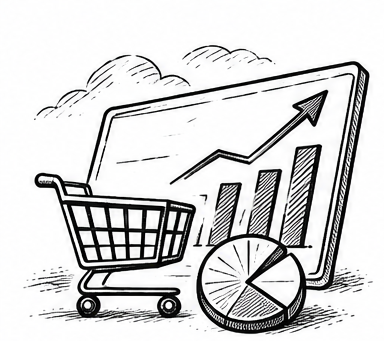
\includegraphics[width=.48\textwidth,height=.28\textheight,keepaspectratio]{../assets/miniportadas/01-resumen-ejecutivo.png}
\vfill
{\normalsize RetailSmart Global\\2026\par}
\end{titlepage}
\hypersetup{pageanchor=true}
\pagenumbering{roman}
\section*{Control de cambios}
\addcontentsline{toc}{section}{Control de cambios}
\begin{tabularx}{\textwidth}{@{}p{.15\textwidth}p{.18\textwidth}X@{}}
\toprule
\textbf{Versión} & \textbf{Fecha} & \textbf{Descripción} \\
\midrule
1.0 & 2026 & Creación del informe técnico de implementación y validación de Lumina Retail. \\
\bottomrule
\end{tabularx}
\clearpage
\tableofcontents
\clearpage
\pagenumbering{arabic}









\clearpage
\section{Resumen ejecutivo}

\begin{center}
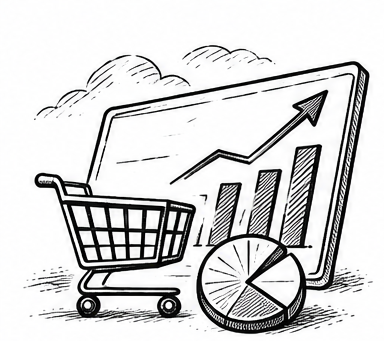
\includegraphics[width=.4704\textwidth]{../assets/miniportadas/01-resumen-ejecutivo.png}
\end{center}

\subsection{Visión ejecutiva y alcance}

RetailSmart Global necesita transformar señales fragmentadas de pedidos, inventario, logística y telemetría en información trazable para decisiones operativas. Lumina Retail implementa una plataforma analítica desacoplada de los sistemas transaccionales. La solución integra \textbf{pipelines de transformación, procesamiento híbrido por lotes y en tiempo real y productos analíticos}, con trazabilidad entre fuentes, procesamiento y consumo.\par

\begingroup\small
\begin{longtable}{@{}>{\raggedright\arraybackslash}p{0.3068\textwidth}>{\raggedright\arraybackslash}p{0.3068\textwidth}>{\raggedright\arraybackslash}p{0.3068\textwidth}@{}}
\toprule
\textbf{Compromiso} & \textbf{Materialización técnica} & \textbf{Resultado esperado} \\
\midrule
\endfirsthead
\toprule
\textbf{Compromiso} & \textbf{Materialización técnica} & \textbf{Resultado esperado} \\
\midrule
\endhead
Procesamiento continuo & Pub/\allowbreak{}Sub → Apache Beam/\allowbreak{}Dataflow → BigQuery Silver; consumo Gold separado & event\_\allowbreak{}id en raw y order\_\allowbreak{}id en Silver \\
Procesamiento por lotes & Landing → BigQuery Bronze/\allowbreak{}Silver/\allowbreak{}Gold, orquestado con Workflows & batch\_\allowbreak{}id y conteos conciliados en cada etapa \\
Integración de datos & Normalización, reglas de calidad y joins por claves sustentadas & Evidencia SQL y resultado antes/\allowbreak{}después \\
Analítica & Productos Gold, Operational Mart, vistas & Esquemas, granularidad y consultas reproducibles \\
\bottomrule
\end{longtable}
\endgroup

\textbf{Límites de la solución:} los sistemas productores empresariales y las aplicaciones consumidoras externas permanecen desacoplados de la plataforma. La predicción de demanda se incorpora como una capacidad analítica de referencia. Los beneficios operativos se evalúan contra una línea base y resultados reproducibles.\par





\clearpage
\section{Contexto empresarial y objetivos}

\begin{center}

\includegraphics[width=.4704\textwidth]{../assets/miniportadas/02-contexto-objetivos.png}
\end{center}

\subsection{Situación empresarial}

La arquitectura responde a cinco problemas documentados: riesgo de quiebre de stock, desalineación geográfica del inventario, saturación operativa, comportamiento fragmentado del cliente y riesgo de fallas de activos. La plataforma habilita cuatro verticales de análisis y recomendación, sin convertirse en sistema transaccional de registro.\par

\begingroup\small
\begin{longtable}{@{}>{\raggedright\arraybackslash}p{0.3068\textwidth}>{\raggedright\arraybackslash}p{0.3068\textwidth}>{\raggedright\arraybackslash}p{0.3068\textwidth}@{}}
\toprule
\textbf{Necesidad} & \textbf{Señal o producto de datos} & \textbf{Dependencia} \\
\midrule
\endfirsthead
\toprule
\textbf{Necesidad} & \textbf{Señal o producto de datos} & \textbf{Dependencia} \\
\midrule
\endhead
Anticipar quiebre & CU01 riesgo de quiebre & pedidos, inventario, SKU, tienda \\
Planificar reposición & CU02 plan de reposición & histórico, stock, predicción \\
Evaluar operación & CU03 KPIs operativos & pedidos, entregas, periodos \\
Priorizar mantenimiento & CU04 alertas de mantenimiento & telemetría y activos \\
\bottomrule
\end{longtable}
\endgroup

\subsection{Alcance de la implementación}

La implementación se organiza en tres capacidades principales: limpieza, enriquecimiento e integración de fuentes; procesamiento híbrido de eventos y lotes; y consolidación de estructuras analíticas. Gobierno, exposición mediante API y predicción complementan estas capacidades.\par

\textbf{Hipótesis de valor:} integrar datos con trazabilidad permite decisiones más oportunas. \textbf{Validación requerida:} medir tiempo de disponibilidad del dato, completitud, duplicados y conciliación por escenario. Los indicadores de servicio se evalúan con mediciones de ejecución y una línea base explícita.\par




\clearpage
\section{Arquitectura de solución}

\begin{center}

\includegraphics[width=.4704\textwidth]{../assets/miniportadas/03-arquitectura-solucion.png}
\end{center}

\subsection{Arquitectura de referencia y arquitectura implementada}

\begin{figure}[htbp]
\centering
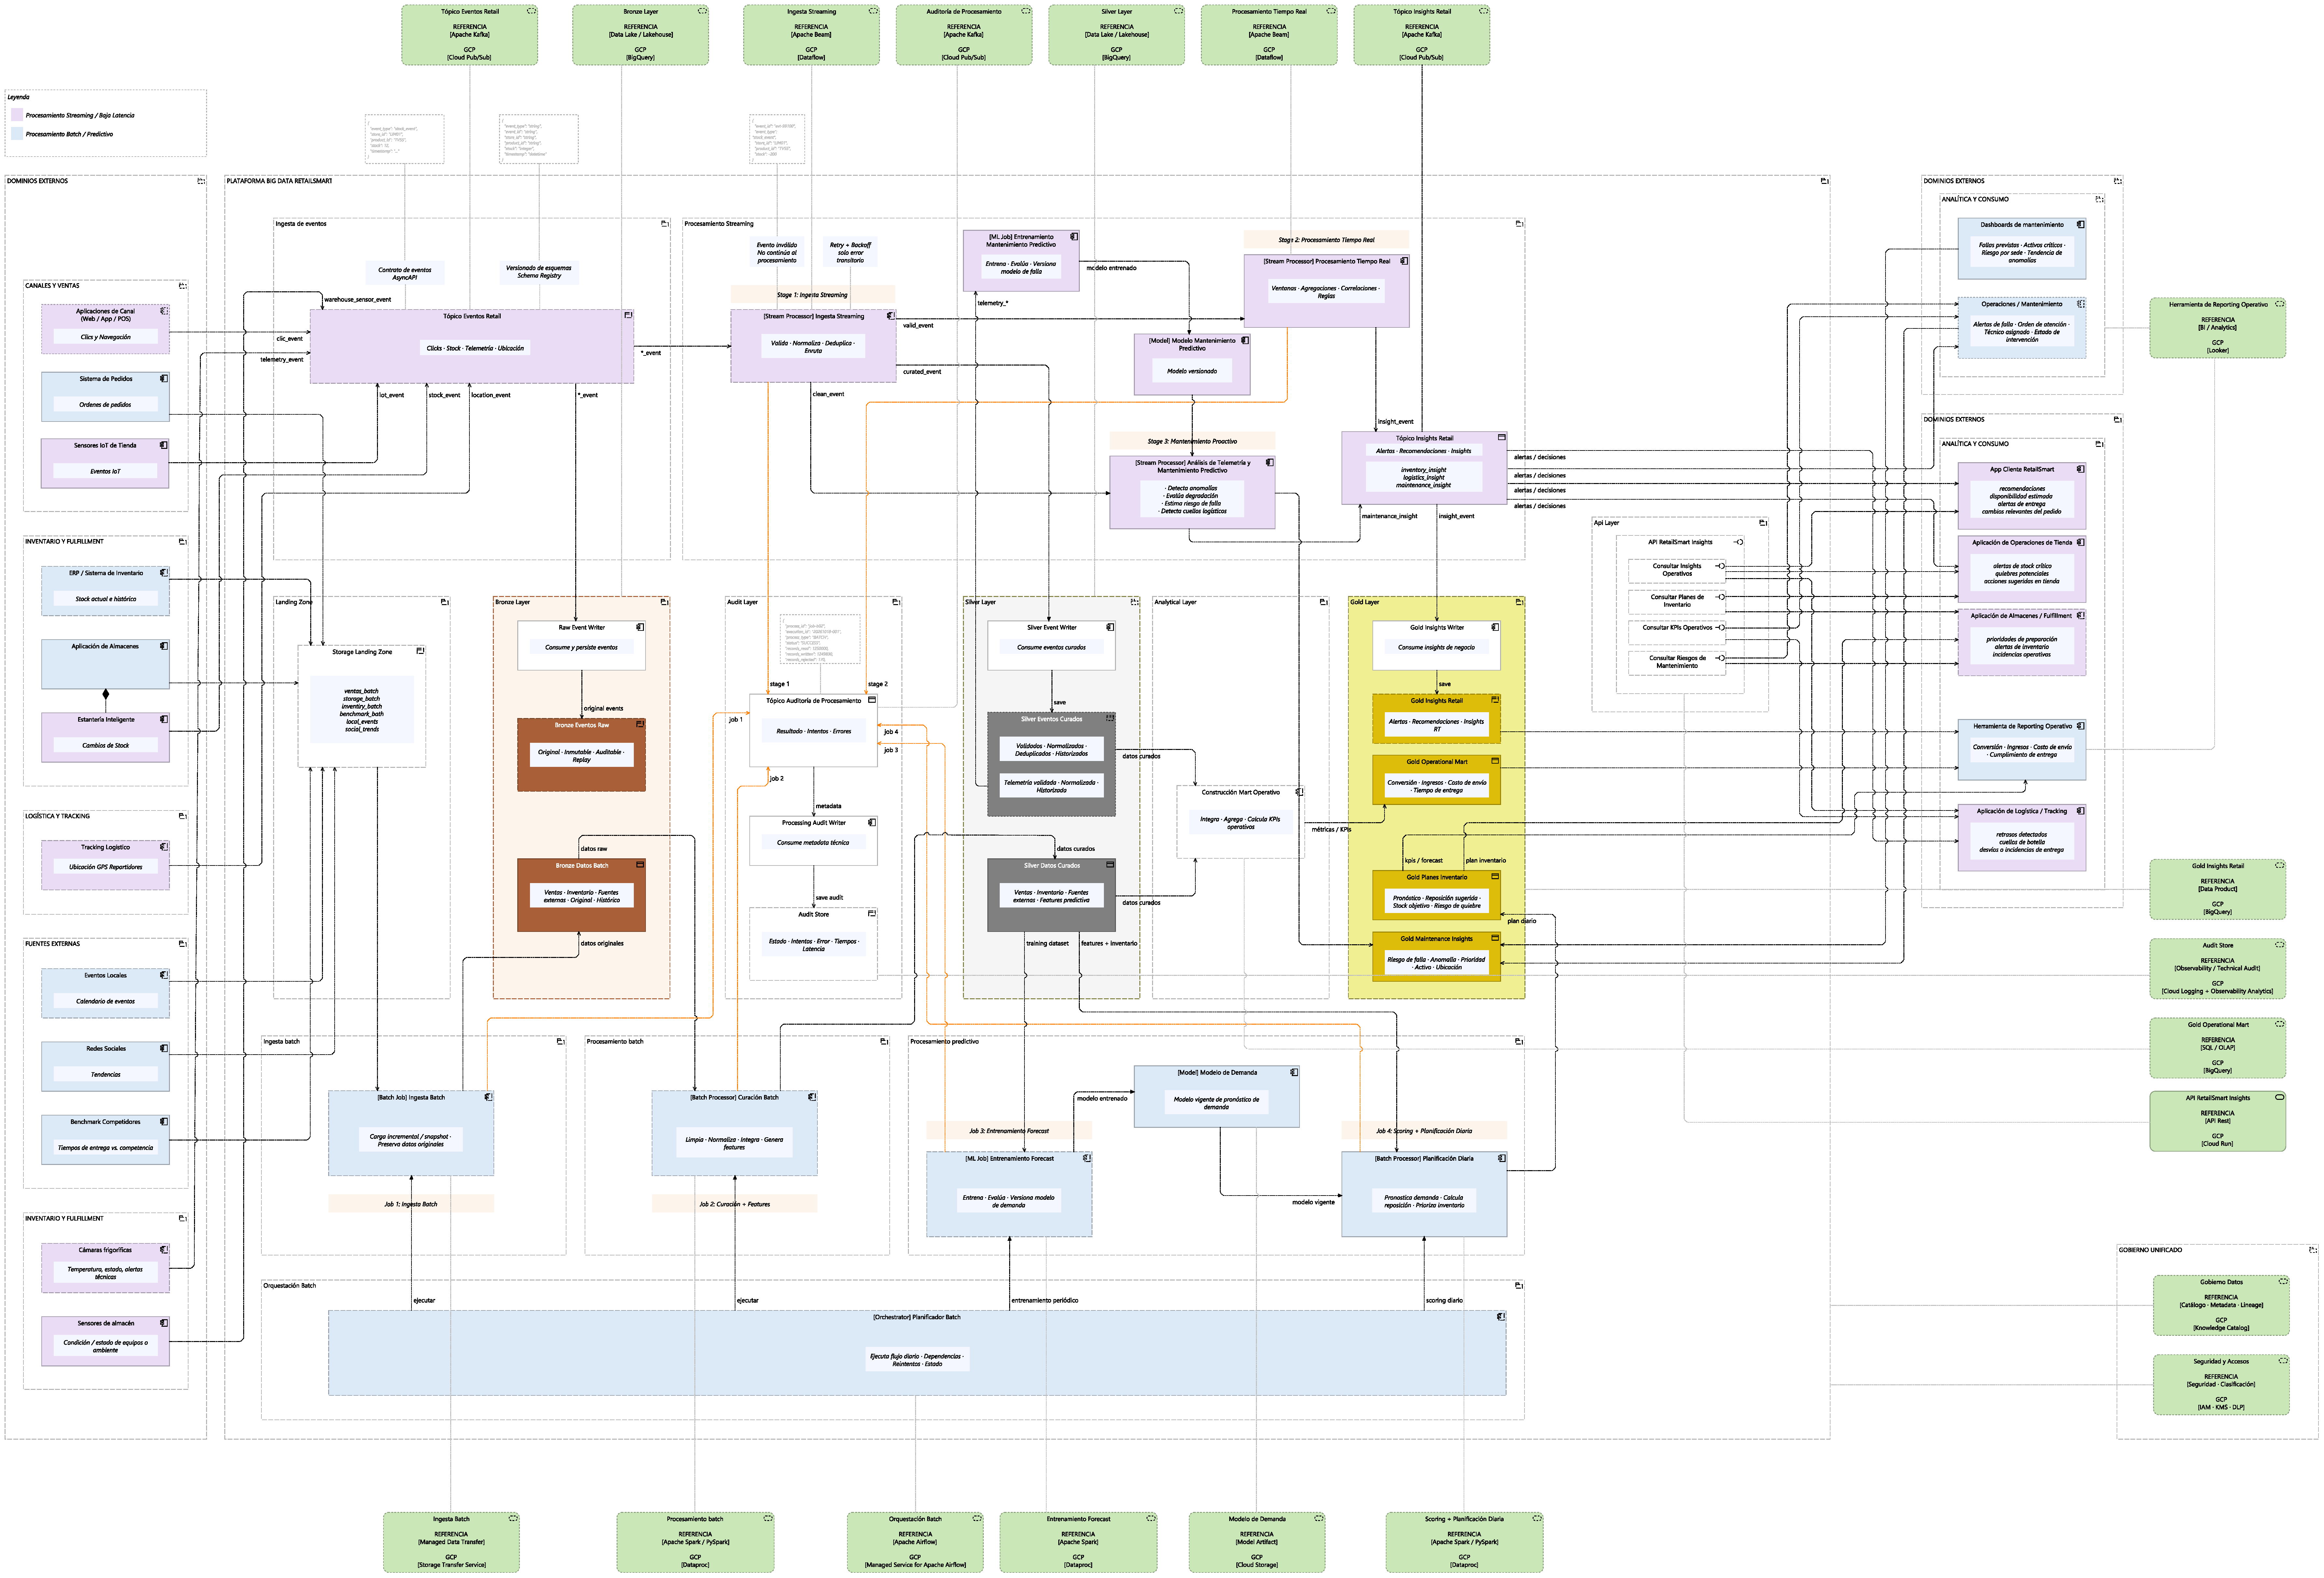
\includegraphics[width=\textwidth,height=.70\textheight,keepaspectratio]{../../../../docs/architecture/generated/arquitectura-archimate.pdf}
\caption{Arquitectura de solución de Lumina Retail}
\end{figure}

La arquitectura de solución describe los componentes, integraciones y responsabilidades de la plataforma. El inventario de servicios y sus configuraciones se presenta en el anexo A.\par

\begingroup\small
\begin{longtable}{@{}>{\raggedright\arraybackslash}p{0.2268\textwidth}>{\raggedright\arraybackslash}p{0.2268\textwidth}>{\raggedright\arraybackslash}p{0.2268\textwidth}>{\raggedright\arraybackslash}p{0.2268\textwidth}@{}}
\toprule
\textbf{Componente} & \textbf{Diseño de referencia} & \textbf{Implementación de Lumina Retail} & \textbf{Consideraciones operativas} \\
\midrule
\endfirsthead
\toprule
\textbf{Componente} & \textbf{Diseño de referencia} & \textbf{Implementación de Lumina Retail} & \textbf{Consideraciones operativas} \\
\midrule
\endhead
Bronze y Silver & Almacenamiento de objetos / Parquet & BigQuery & SQL unificado y acceso analítico; controlar costos de almacenamiento y consultas \\
Landing & Cloud Storage & Cloud Storage & Conservación de archivos de entrada y URI de origen \\
Mensajería & Pub/\allowbreak{}Sub & Pub/\allowbreak{}Sub & Suscripciones independientes para raw y procesamiento \\
Streaming & Beam/\allowbreak{}Dataflow & Beam/\allowbreak{}Dataflow & Separación de transporte, validación y escritura \\
Batch & Procesamiento por lotes & Workflows + BigQuery SQL & Orquestación y materialización; Dataproc es una ruta de cómputo separada \\
Exposición & Productos analíticos & BigQuery Gold + Cloud Run privado & Lectura IAM y API sin consumidor externo aprovisionado \\
\bottomrule
\end{longtable}
\endgroup

\textbf{Control operativo:} la ejecución de los servicios se complementa con conciliaciones de registros y comprobación de los datos materializados. El estado de infraestructura y la integridad del dato se supervisan por separado.\par


\begin{figure}[htbp]
\centering
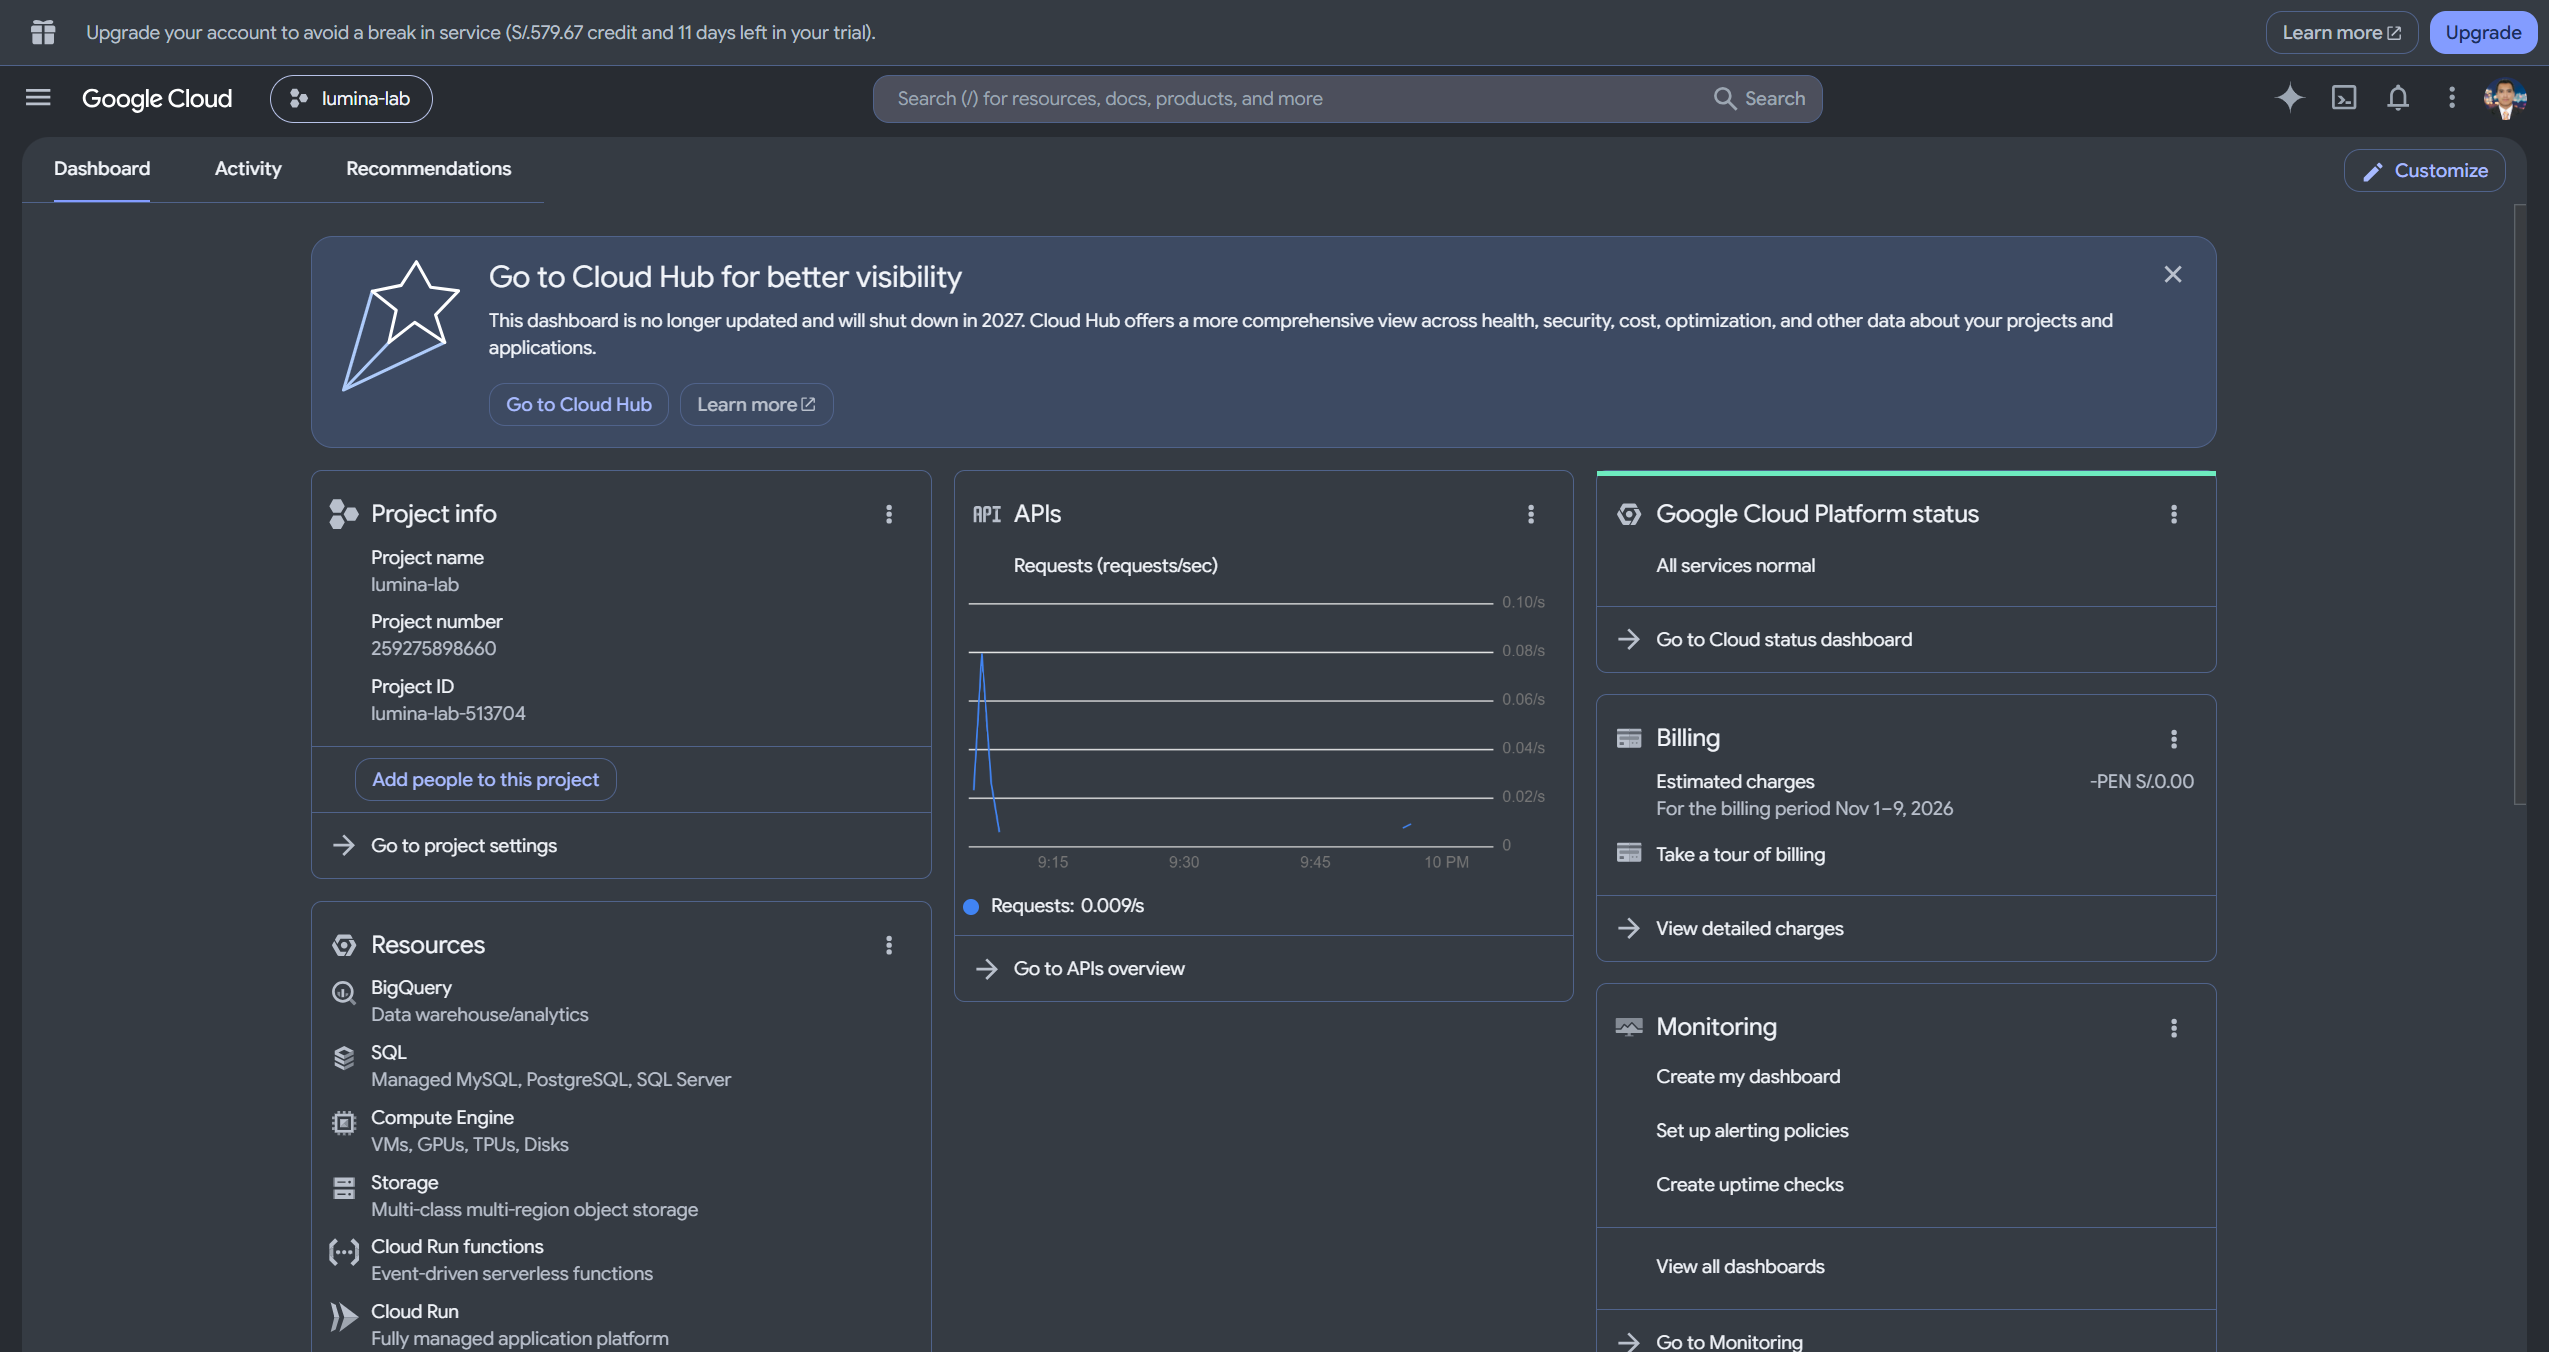
\includegraphics[width=0.96\textwidth]{../assets/evidencia/01-fundacion/01-inventario-servicios.png}
\caption{Vista de Inventario de servicios GCP}
\end{figure}






\clearpage
\section{Fuentes, contratos y arquitectura de datos}

\begin{center}
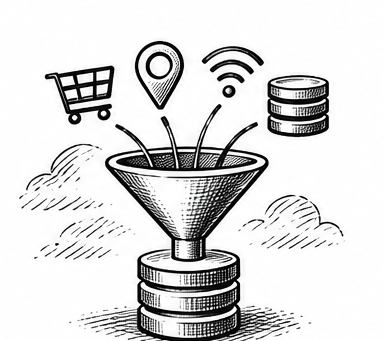
\includegraphics[width=.4704\textwidth]{../assets/miniportadas/04-fuentes-contratos.png}
\end{center}

\subsection{Fuentes propias y contratos de generación}

La implementación utiliza \textbf{exclusivamente conjuntos de datos y eventos ad hoc generados para Lumina Retail}. No se han ingerido datasets públicos ni conectado fuentes externas reales. Las familias descritas representan escenarios de negocio simulados y se procesan mediante los contratos y pipelines propios de la plataforma.\par



\begingroup\small
\begin{longtable}{@{}>{\raggedright\arraybackslash}p{0.2268\textwidth}>{\raggedright\arraybackslash}p{0.2268\textwidth}>{\raggedright\arraybackslash}p{0.2268\textwidth}>{\raggedright\arraybackslash}p{0.2268\textwidth}@{}}
\toprule
\textbf{Familia} & \textbf{Fuente de datos} & \textbf{Aplicación en la solución} & \textbf{Precaución} \\
\midrule
\endfirsthead
\toprule
\textbf{Familia} & \textbf{Fuente de datos} & \textbf{Aplicación en la solución} & \textbf{Precaución} \\
\midrule
\endhead
Datos operativos ad hoc & pedidos, inventario y entregas generados para Lumina Retail & cargas batch y modelado analítico & Conservar identificadores, granularidad y versión de generación \\
Datos contextuales ad hoc & benchmark de competidores, eventos locales y redes sociales generados para escenarios controlados & enriquecimiento batch & Identificar cada conjunto como dato sintético, no como extracción externa \\
Eventos operativos ad hoc & pedidos, inventario, sensores y telemetría producidos por generadores propios & procesamiento streaming & Correlacionar evento, escenario y ejecución \\
\bottomrule
\end{longtable}
\endgroup

\subsection{Contrato lógico de evento}

El generador publica un mensaje JSON con el siguiente contrato de referencia, definido en docs/\allowbreak{}arquitectura/\allowbreak{}contrato-evento-original.json:\par

\begingroup\small
\begin{longtable}{@{}>{\raggedright\arraybackslash}p{0.2268\textwidth}>{\raggedright\arraybackslash}p{0.2268\textwidth}>{\raggedright\arraybackslash}p{0.2268\textwidth}>{\raggedright\arraybackslash}p{0.2268\textwidth}@{}}
\toprule
\textbf{Campo de entrada} & \textbf{Tipo} & \textbf{Propósito} & \textbf{Ejemplo del contrato} \\
\midrule
\endfirsthead
\toprule
\textbf{Campo de entrada} & \textbf{Tipo} & \textbf{Propósito} & \textbf{Ejemplo del contrato} \\
\midrule
\endhead
schema\_\allowbreak{}version & string & versión del esquema & 1.1.0 \\
simulation\_\allowbreak{}id / scenario\_\allowbreak{}id & string & correlación de simulación y escenario & sim-20261103-001 / black-friday \\
producer\_\allowbreak{}id / event\_\allowbreak{}type & string & productor y tipo de evento & channel-apps / order\_\allowbreak{}created \\
event\_\allowbreak{}id / trace\_\allowbreak{}id & string & identidad y seguimiento & evt-000001 / trace-order-000001 \\
occurred\_\allowbreak{}at / emitted\_\allowbreak{}at & string ISO 8601 & tiempos de negocio y emisión & 2026-11-03T10:00:00Z \\
payload & objeto JSON & atributos del pedido & order\_\allowbreak{}id, order\_\allowbreak{}line\_\allowbreak{}id, customer\_\allowbreak{}id, store\_\allowbreak{}id, product\_\allowbreak{}id, quantity \\
\bottomrule
\end{longtable}
\endgroup

\textbf{Correspondencia streaming:} la app representa los seis productores definidos en ArchiMate. Pub/Sub recibe sus eventos; Dataflow valida el envelope y enruta cada tipo a su entidad Silver. En pedidos, convierte explícitamente \texttt{product\_id} a \texttt{sku\_id}. El detalle de campos obligatorios y salidas está en el anexo B.\par

\begingroup\small
\begin{longtable}{@{}>{\raggedright\arraybackslash}p{0.2268\textwidth}>{\raggedright\arraybackslash}p{0.2268\textwidth}>{\raggedright\arraybackslash}p{0.2268\textwidth}>{\raggedright\arraybackslash}p{0.2268\textwidth}@{}}
\toprule
\textbf{Productor ArchiMate} & \textbf{Evento / campos clave} & \textbf{Entrada GCP} & \textbf{Salida Dataflow} \\
\midrule
\endfirsthead
\toprule
\textbf{Productor ArchiMate} & \textbf{Evento / campos clave} & \textbf{Entrada GCP} & \textbf{Salida Dataflow} \\
\midrule
\endhead
Canales Web/App/POS & order\_created; order\_id, order\_line\_id, product\_id, quantity & Pub/Sub & Silver.pedidos \\
Cámaras frigoríficas & cold\_\allowbreak{}chain\_\allowbreak{}reading; asset\_id, sensor\_id, warehouse\_id, metric\_value, unit & Pub/Sub & Silver.telemetria\_\allowbreak{}activos \\
Estantería inteligente & inventory\_\allowbreak{}level\_\allowbreak{}changed; snapshot\_id, warehouse\_id, sku\_id, on\_hand\_qty, reserved\_qty & Pub/Sub & Silver.inventario \\
Sensores IoT de tienda & store\_\allowbreak{}sensor\_\allowbreak{}reading; asset\_id, sensor\_id, store\_id, metric\_value, unit & Pub/Sub & Silver.telemetria\_\allowbreak{}activos \\
Sensores de almacén & warehouse\_\allowbreak{}sensor\_\allowbreak{}reading; asset\_id, sensor\_id, warehouse\_id, metric\_value, unit & Pub/Sub & Silver.telemetria\_\allowbreak{}activos \\
Tracking logístico & delivery\_\allowbreak{}status\_\allowbreak{}changed; delivery\_id, order\_id, delivered\_at & Pub/Sub & Silver.entregas \\
\bottomrule
\end{longtable}
\endgroup
\par

\subsection{Medallion físico}

\begingroup\small
\begin{longtable}{@{}>{\raggedright\arraybackslash}p{0.3068\textwidth}>{\raggedright\arraybackslash}p{0.3068\textwidth}>{\raggedright\arraybackslash}p{0.3068\textwidth}@{}}
\toprule
\textbf{Capa} & \textbf{Servicio} & \textbf{Responsabilidad} \\
\midrule
\endfirsthead
\toprule
\textbf{Capa} & \textbf{Servicio} & \textbf{Responsabilidad} \\
\midrule
\endhead
Landing & Cloud Storage & archivos batch, URI y staging \\
Bronze & BigQuery & raw Pub/\allowbreak{}Sub, JSON, metadata y lotes \\
Silver & BigQuery & entidades tipadas, normalizadas, con calidad \\
Gold & BigQuery & CU01-CU04, predicciones, Mart y vistas \\
\bottomrule
\end{longtable}
\endgroup

\subsection{Contrato de metadatos por modalidad}

\begingroup\small
\begin{longtable}{@{}>{\raggedright\arraybackslash}p{0.2268\textwidth}>{\raggedright\arraybackslash}p{0.2268\textwidth}>{\raggedright\arraybackslash}p{0.2268\textwidth}>{\raggedright\arraybackslash}p{0.2268\textwidth}@{}}
\toprule
\textbf{Modalidad} & \textbf{Identificador de entrada} & \textbf{Metadatos conservados} & \textbf{Destino} \\
\midrule
\endfirsthead
\toprule
\textbf{Modalidad} & \textbf{Identificador de entrada} & \textbf{Metadatos conservados} & \textbf{Destino} \\
\midrule
\endhead
Streaming & event\_\allowbreak{}id, trace\_\allowbreak{}id & message\_\allowbreak{}id, publish\_\allowbreak{}time, subscription\_\allowbreak{}name, attributes & BigQuery Bronze raw \\
Batch & batch\_\allowbreak{}id, file\_\allowbreak{}id, source\_\allowbreak{}row\_\allowbreak{}number & source\_\allowbreak{}file\_\allowbreak{}uri, source\_\allowbreak{}system, ingested\_\allowbreak{}at, record\_\allowbreak{}hash, is\_\allowbreak{}valid, error\_\allowbreak{}reason & BigQuery Bronze *\_\allowbreak{}raw \\
Curación & clave de negocio del dominio & campos tipados y quality\_\allowbreak{}status & BigQuery Silver \\
\bottomrule
\end{longtable}
\endgroup

El diccionario físico completo se mantiene en el anexo D.\par


\begin{figure}[htbp]
\centering
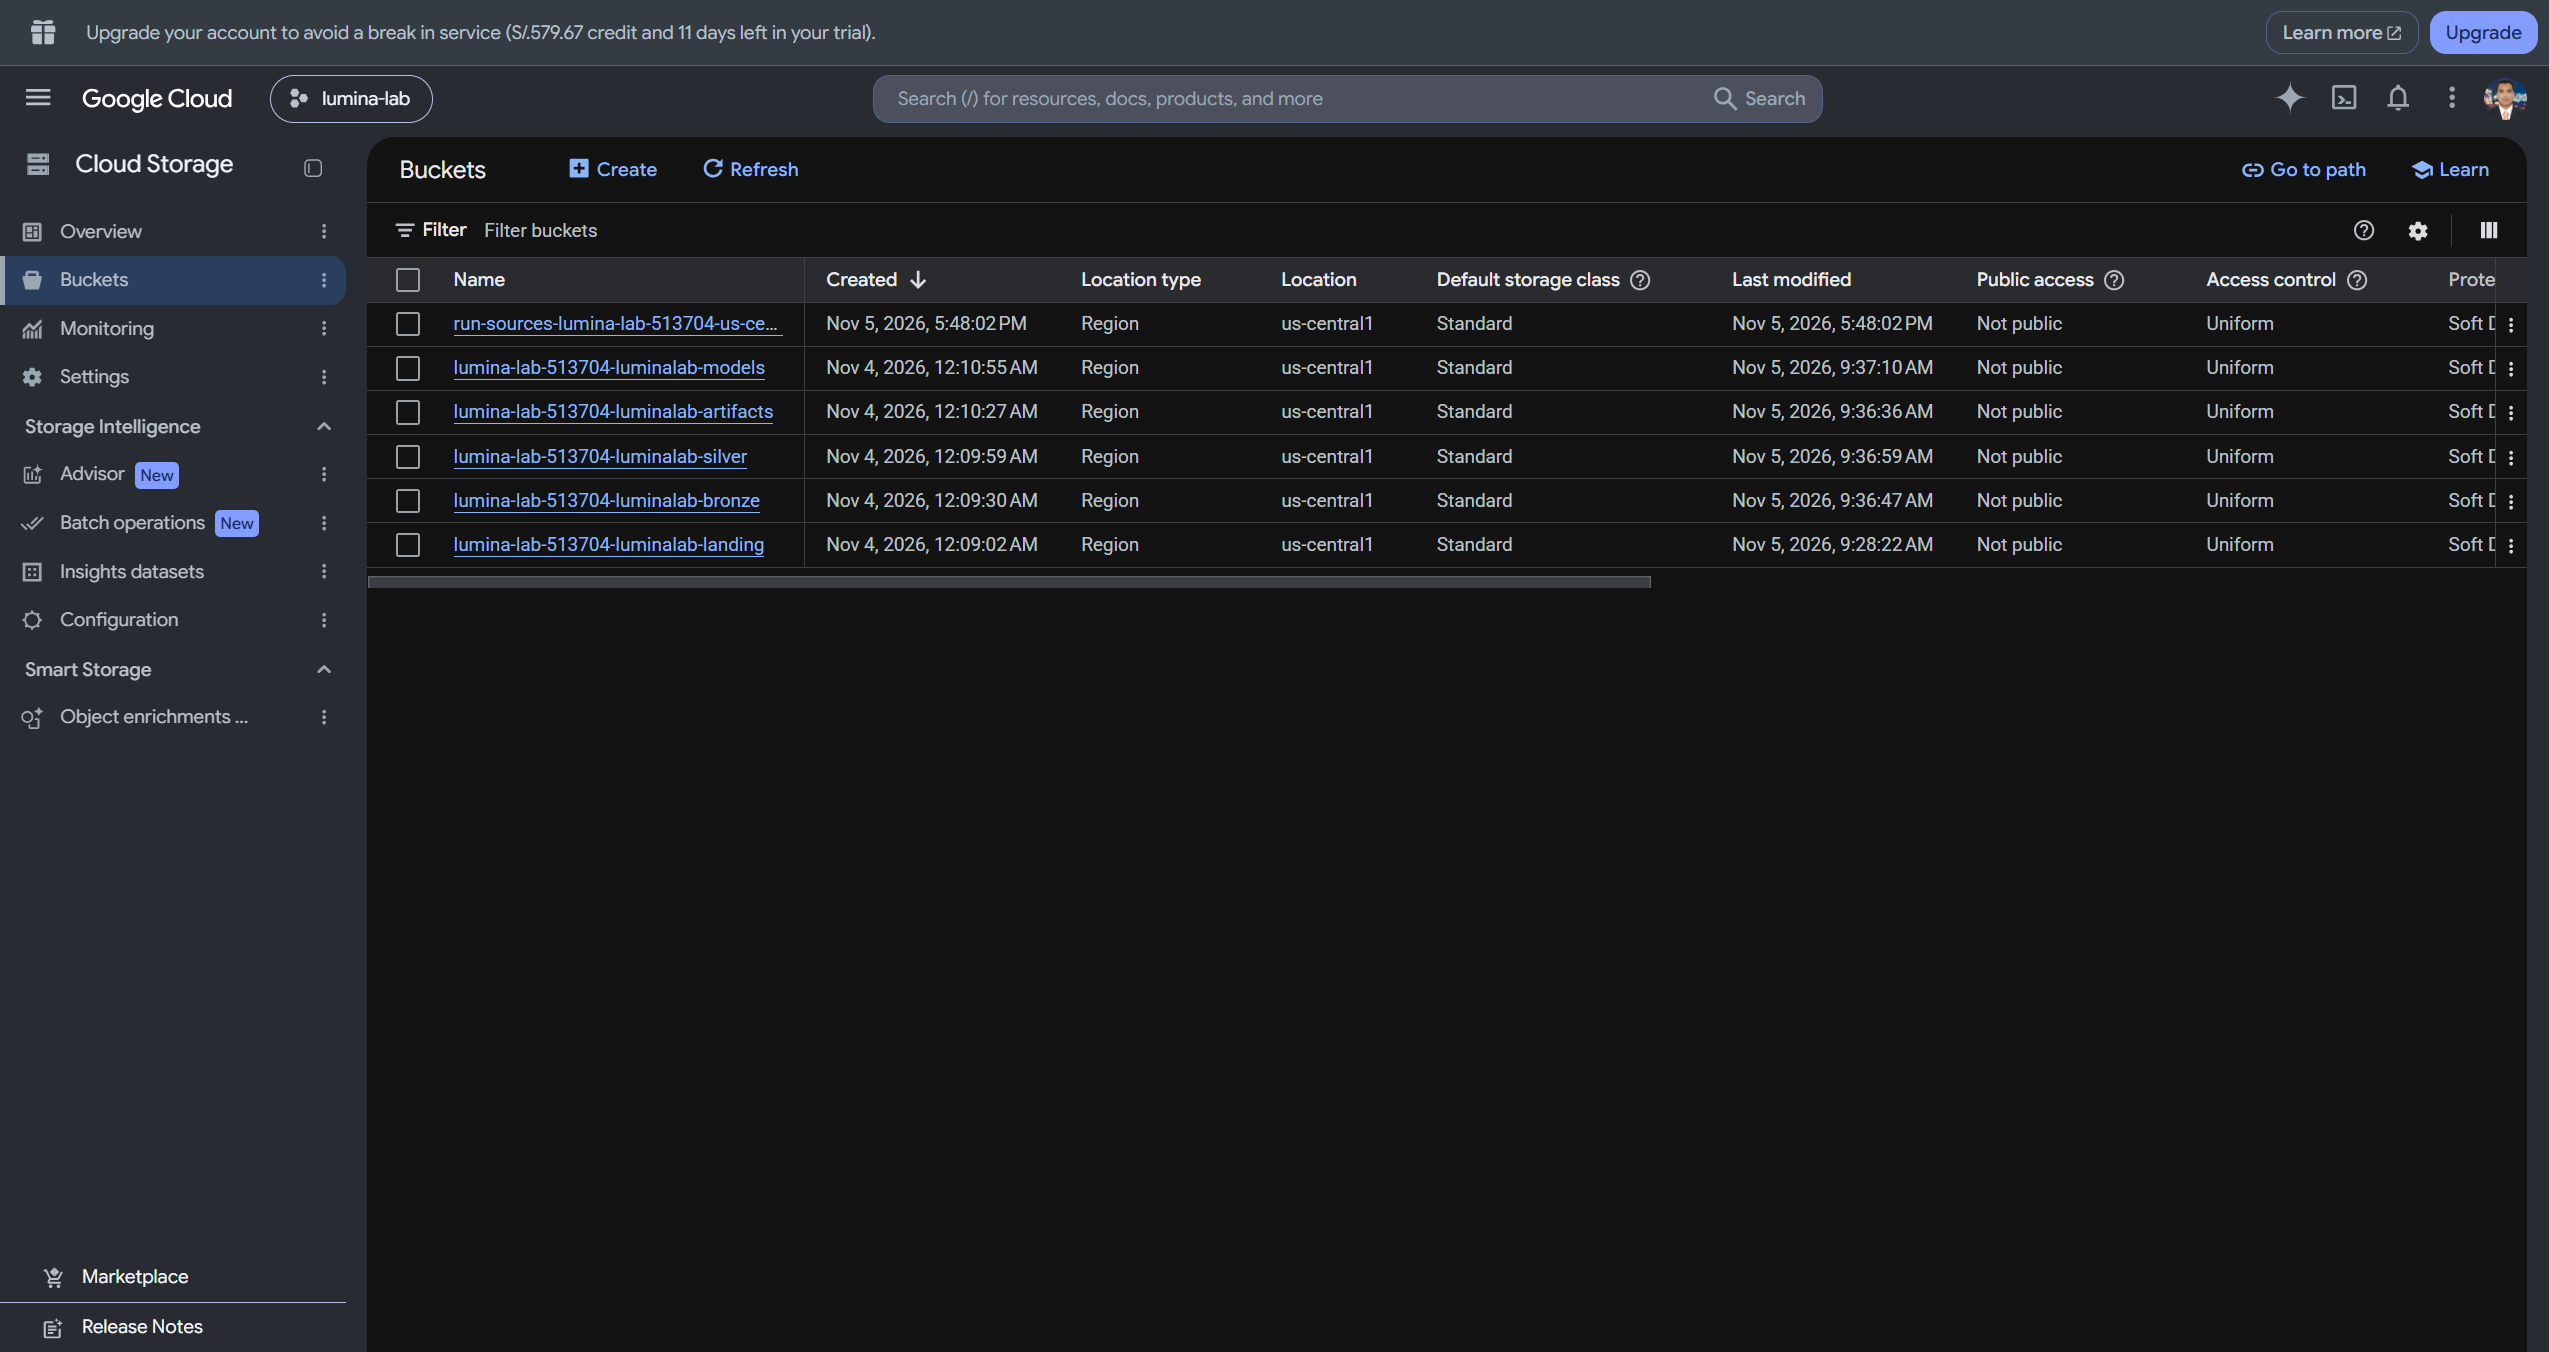
\includegraphics[width=0.96\textwidth]{../assets/evidencia/01-fundacion/02-storage-buckets.png}
\caption{Vista de Buckets de Landing y artefactos}
\end{figure}



\begin{figure}[htbp]
\centering
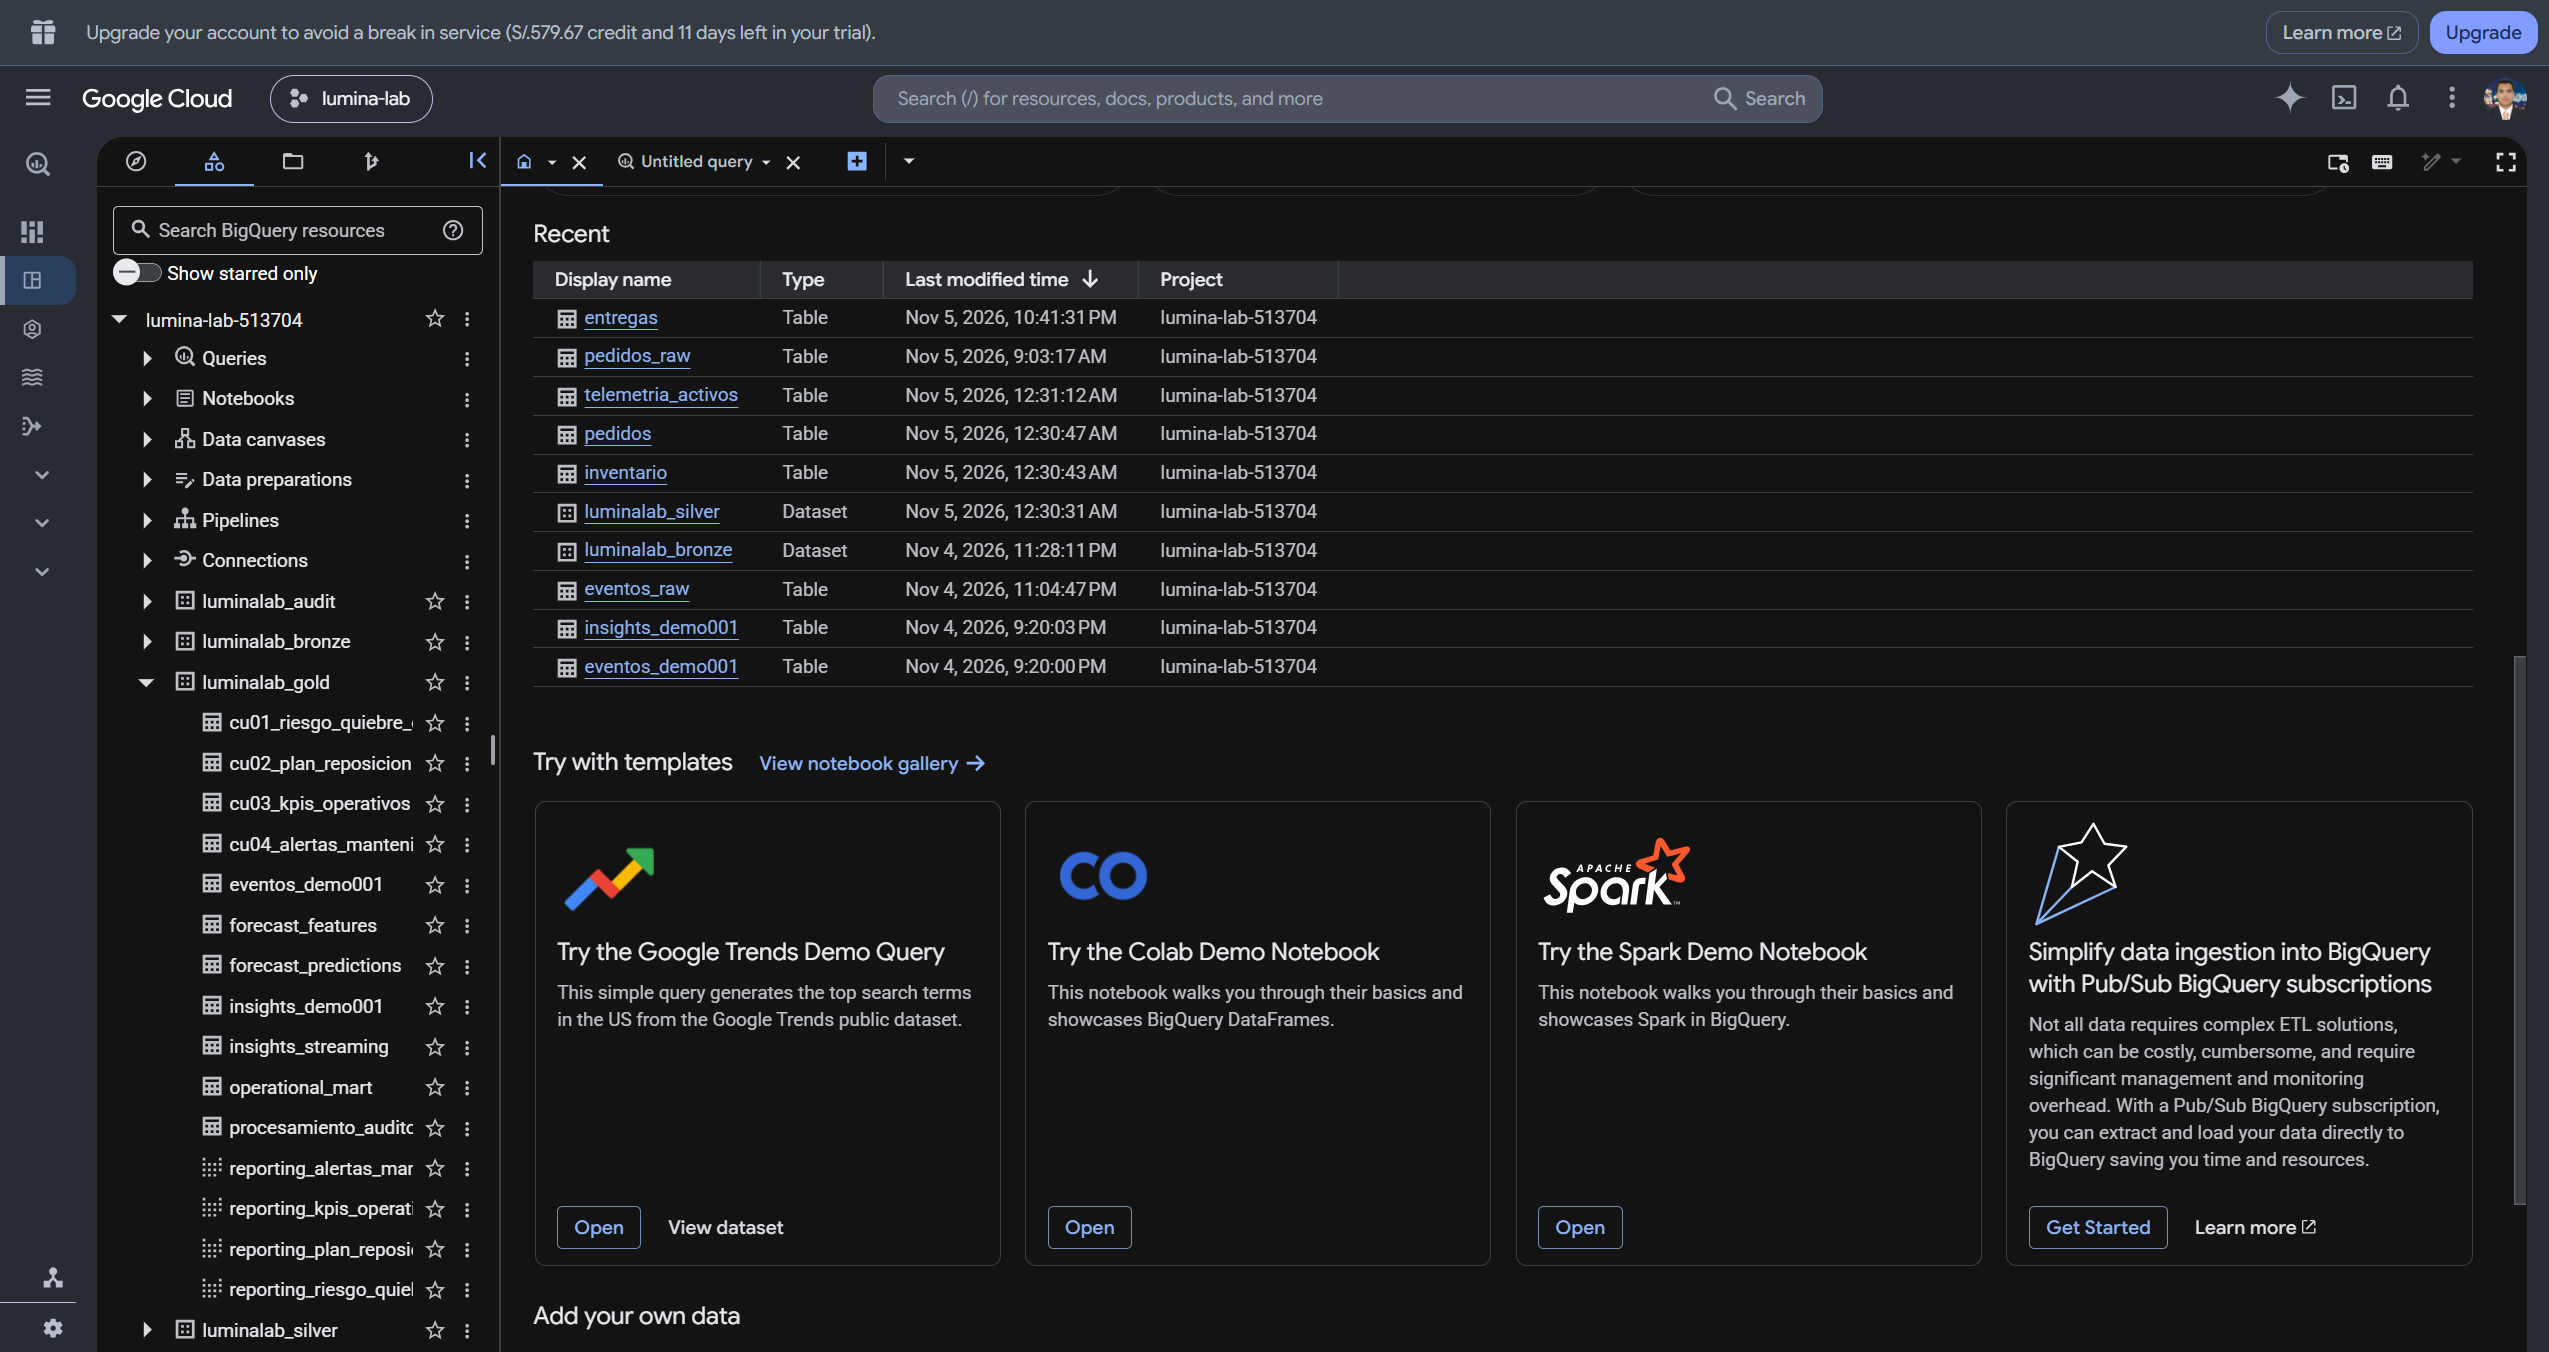
\includegraphics[width=0.96\textwidth]{../assets/evidencia/01-fundacion/03-bigquery-medallion.png}
\caption{Vista de Datasets Bronze, Silver y Gold}
\end{figure}






\clearpage
\section{Implementación de pipelines streaming}

\begin{center}

\includegraphics[width=.4704\textwidth]{../assets/miniportadas/05-streaming.png}
\end{center}

\subsection{Bifurcación del tópico de entrada}

La publicación se entrega a tres suscripciones independientes: raw en BigQuery, archivo JSONL en Cloud Storage y procesamiento Beam/Dataflow hacia Silver. La confirmación del publicador acredita recepción en Pub/Sub; no confirma por sí sola la escritura en Bronze o Silver.\par

\begingroup\small
\begin{longtable}{@{}>{\raggedright\arraybackslash}p{0.2268\textwidth}>{\raggedright\arraybackslash}p{0.2268\textwidth}>{\raggedright\arraybackslash}p{0.2268\textwidth}>{\raggedright\arraybackslash}p{0.2268\textwidth}@{}}
\toprule
\textbf{Etapa} & \textbf{Entrada} & \textbf{Operación} & \textbf{Salida / control} \\
\midrule
\endfirsthead
\toprule
\textbf{Etapa} & \textbf{Entrada} & \textbf{Operación} & \textbf{Salida / control} \\
\midrule
\endhead
Publicación & JSON de evento & Validación contractual de origen & event\_\allowbreak{}id y messageId \\
Raw & Suscripción BigQuery & Persistencia del mensaje & Bronze.eventos\_\allowbreak{}raw\_\allowbreak{}pubsub \\
Curación & Suscripción Dataflow & Validación y enrutamiento por event\_\allowbreak{}type & Silver.pedidos, inventario, entregas o telemetría \\
Consumo & entidades Silver & proceso separado por producto & Gold según su materializador \\
Control & IDs y consultas GCP & verificar cada etapa & ack Pub/Sub no confirma escritura en Bronze/Silver \\
\bottomrule
\end{longtable}
\endgroup

\textbf{Trazabilidad:} el evento raw conserva event\_\allowbreak{}id; Silver.pedidos conserva order\_\allowbreak{}id y order\_\allowbreak{}line\_\allowbreak{}id. La correlación se realiza mediante esas claves. Dataflow termina en Silver; Gold se materializa por procesos separados.\par

\subsection{Contrato de salida de Insights y auditoría}

\begingroup\small
\begin{longtable}{@{}>{\raggedright\arraybackslash}p{0.2268\textwidth}>{\raggedright\arraybackslash}p{0.2268\textwidth}>{\raggedright\arraybackslash}p{0.2268\textwidth}>{\raggedright\arraybackslash}p{0.2268\textwidth}@{}}
\toprule
\textbf{Producto Gold} & \textbf{Entrada} & \textbf{Campos de salida} & \textbf{Clave de correlación} \\
\midrule
\endfirsthead
\toprule
\textbf{Producto Gold} & \textbf{Entrada} & \textbf{Campos de salida} & \textbf{Clave de correlación} \\
\midrule
\endhead
insights\_\allowbreak{}streaming & eventos del pipeline de Insights & insight\_\allowbreak{}id, event\_\allowbreak{}id, insight\_\allowbreak{}type, sku\_\allowbreak{}id, store\_\allowbreak{}id, score, created\_\allowbreak{}at, status & event\_\allowbreak{}id \\
procesamiento\_\allowbreak{}auditoria & procesamiento de eventos & audit\_\allowbreak{}id, event\_\allowbreak{}id, component, status, observed\_\allowbreak{}at, detail & event\_\allowbreak{}id \\
\bottomrule
\end{longtable}
\endgroup

El segundo tópico y su Dataflow producen Gold.insights\_\allowbreak{}streaming y Gold.procesamiento\_\allowbreak{}auditoria. Se exige la misma correlación en ambas. Si no se observa EVENTO\_\allowbreak{}RECIBIDO o INSIGHT\_\allowbreak{}GENERADO, registrar el caso como no verificado, aunque el job esté RUNNING.\par


\begin{figure}[htbp]
\centering
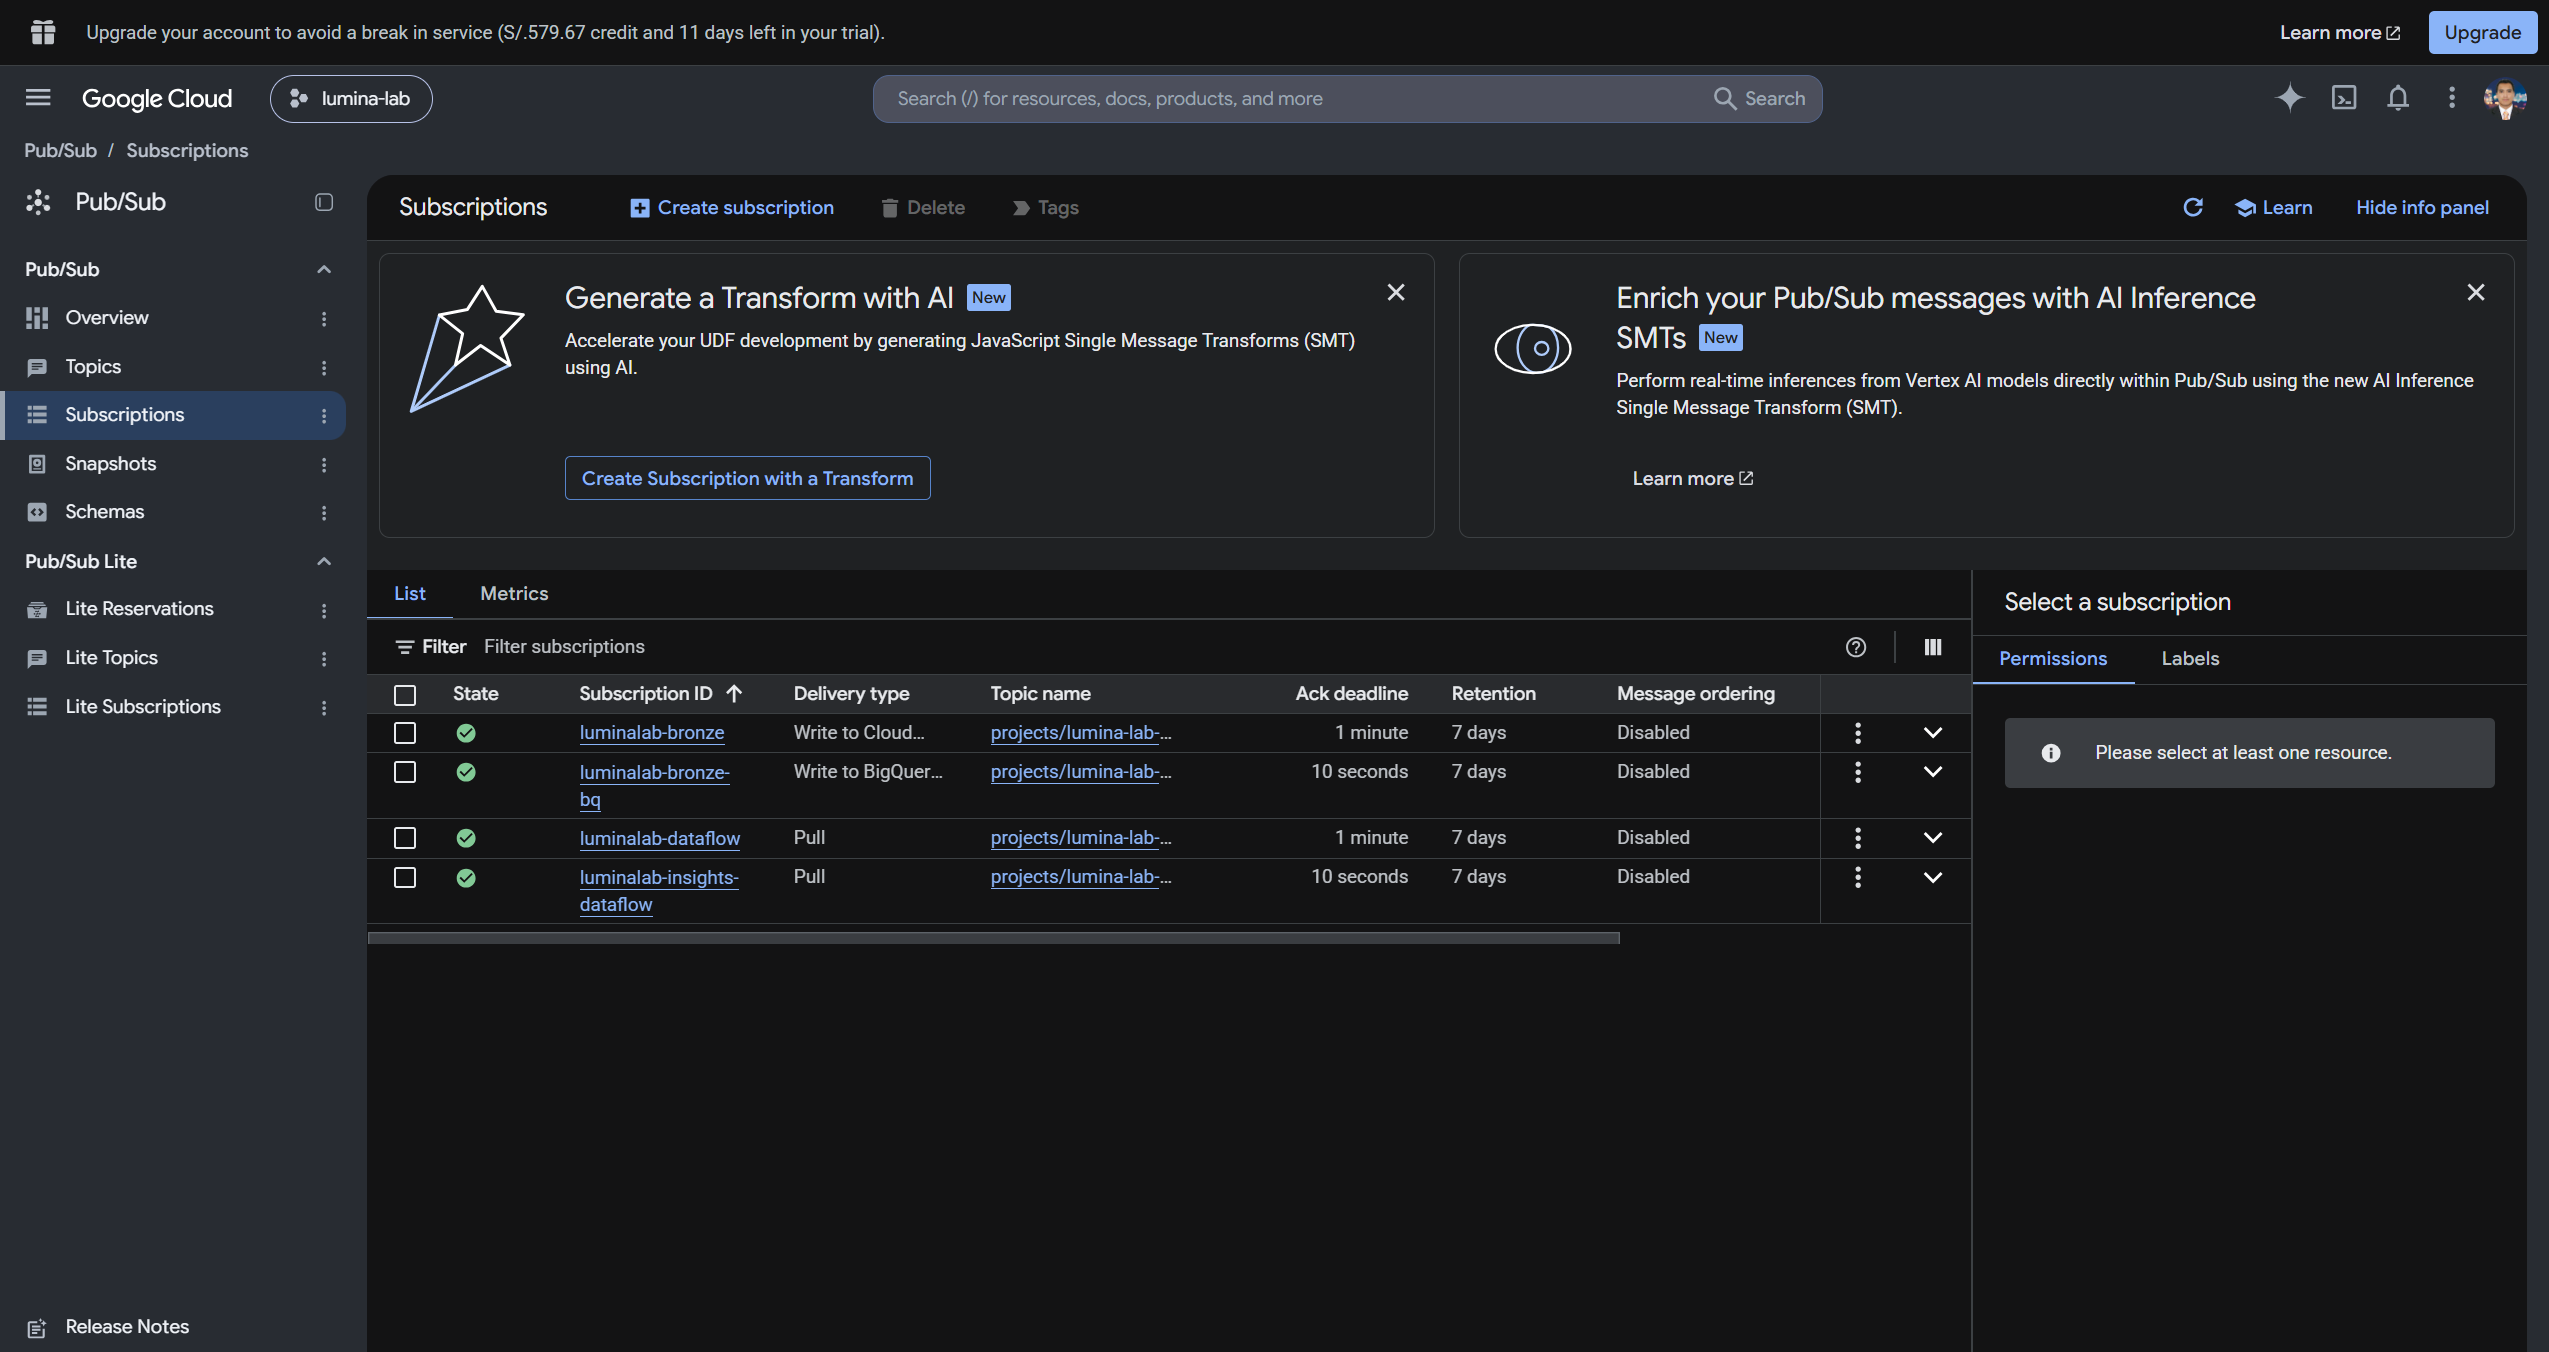
\includegraphics[width=0.96\textwidth]{../assets/evidencia/02-streaming/01-pubsub-topico-suscripciones.png}
\caption{Vista de Tópico y suscripciones}
\end{figure}



\begin{figure}[htbp]
\centering
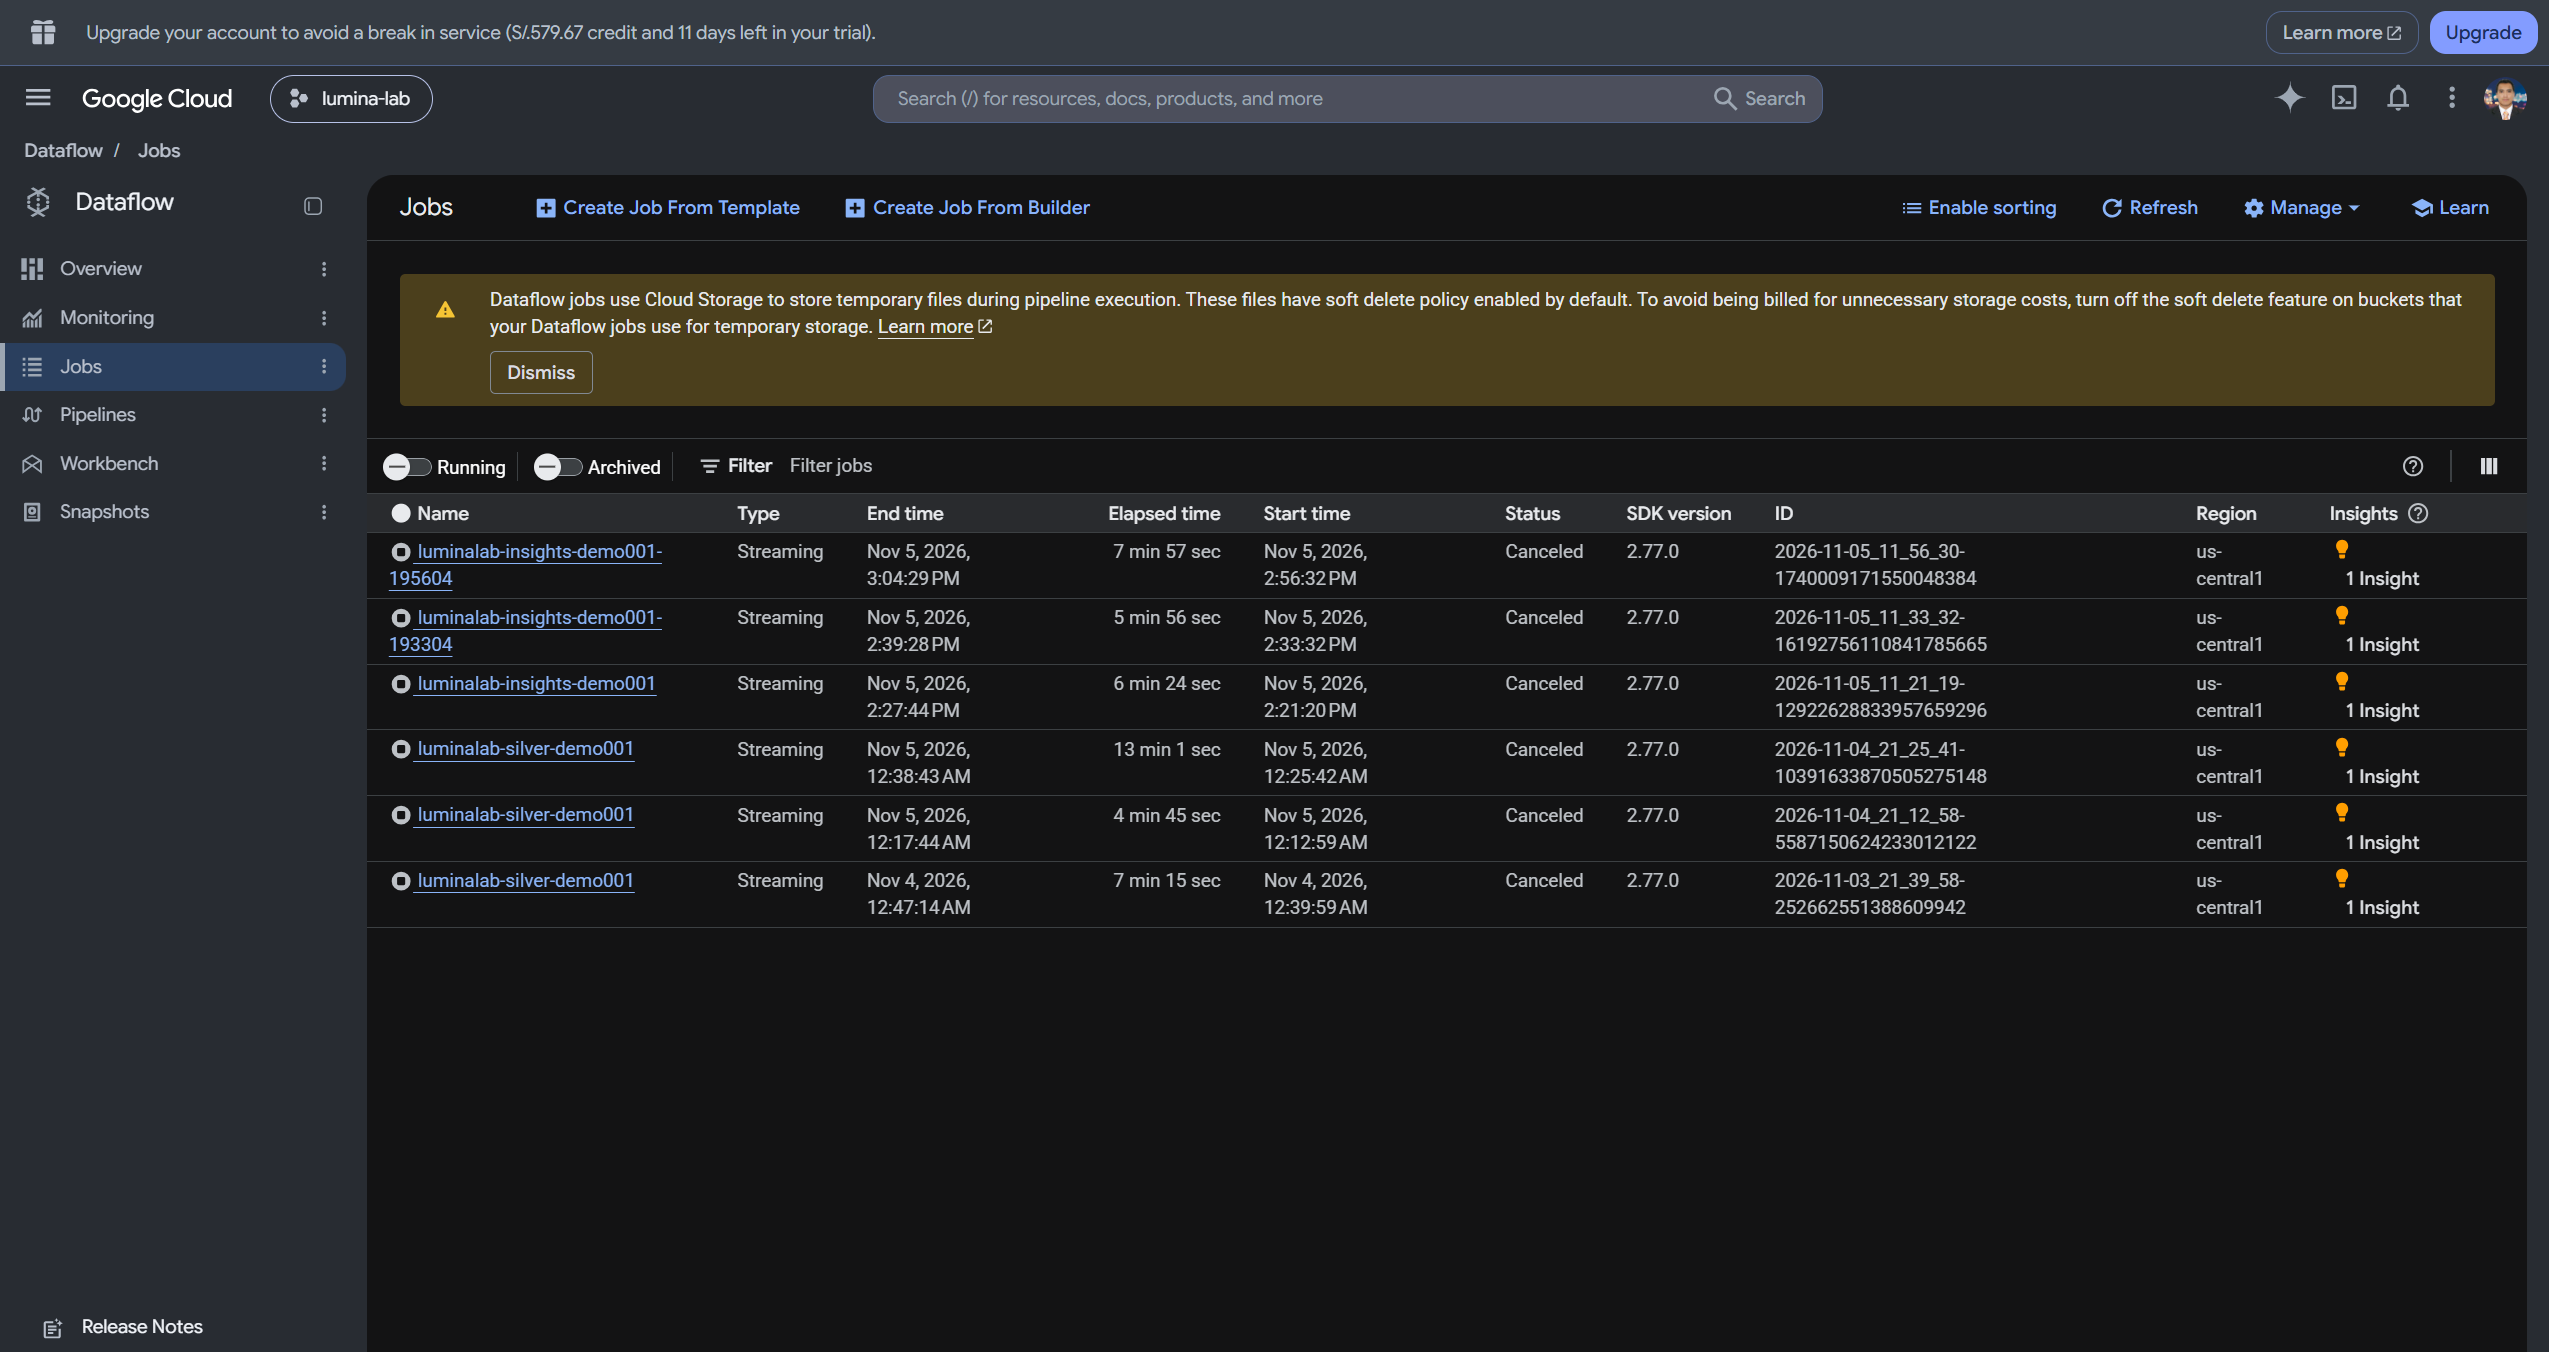
\includegraphics[width=0.96\textwidth]{../assets/evidencia/02-streaming/02-dataflow-job.png}
\caption{Vista de Ejecución Dataflow}
\end{figure}



\begin{figure}[htbp]
\centering
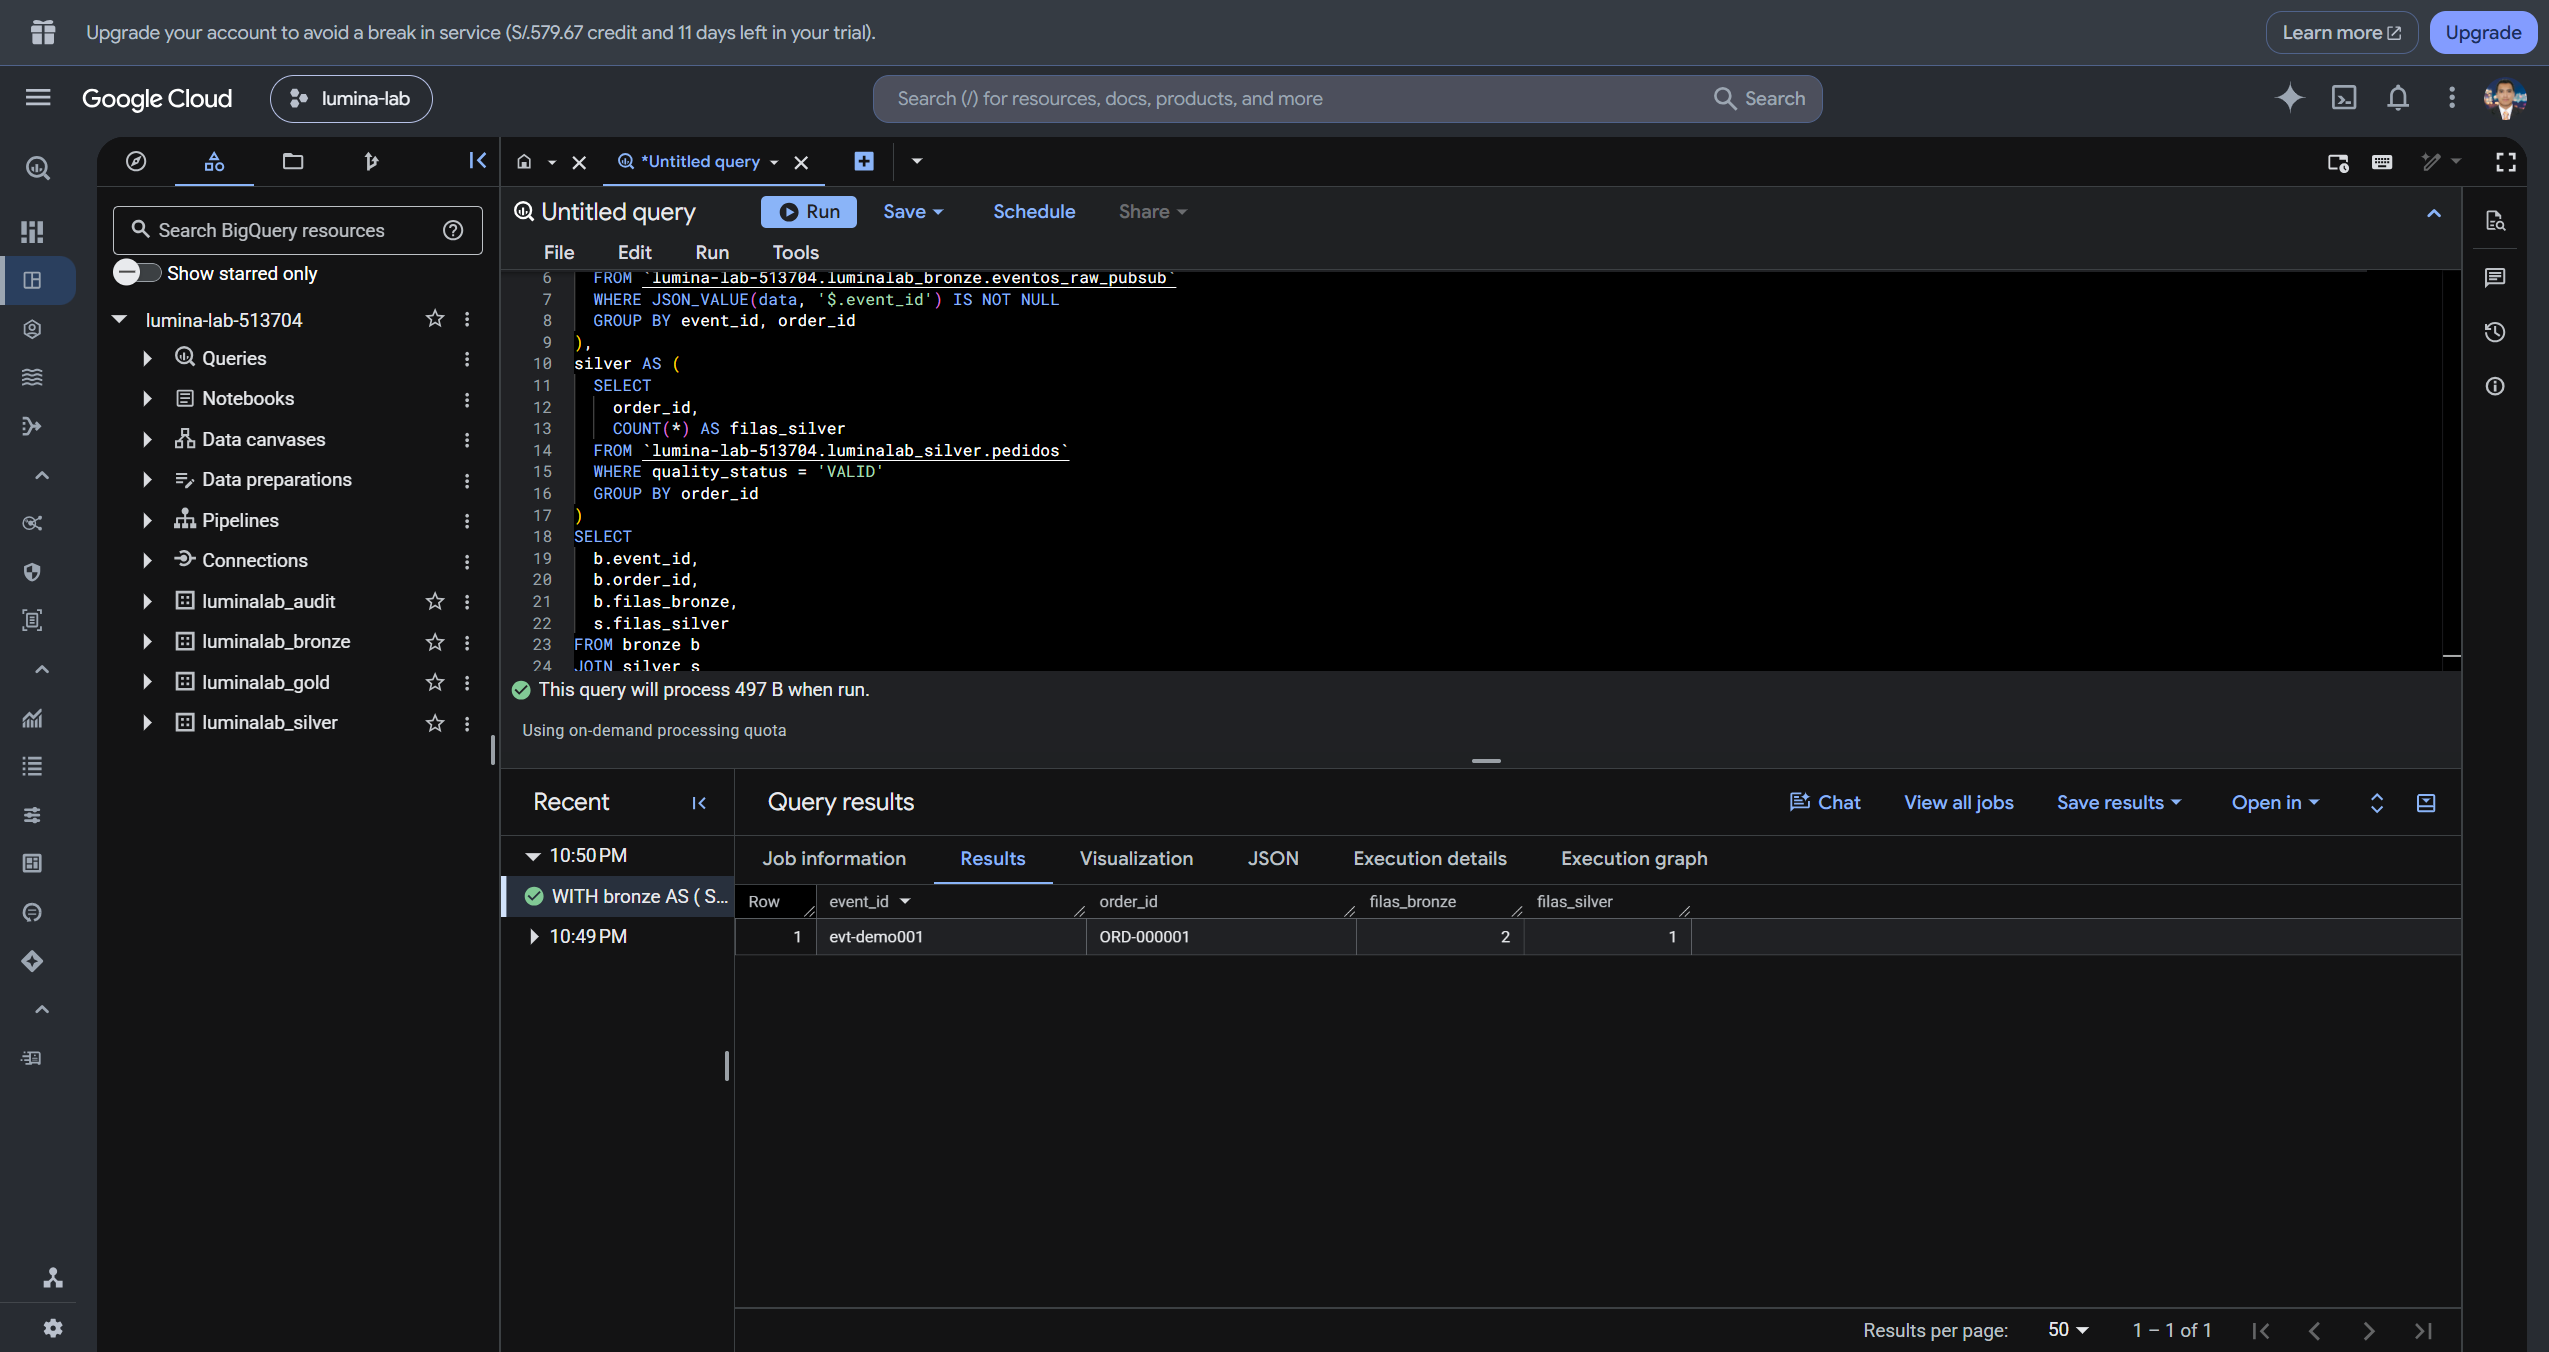
\includegraphics[width=0.96\textwidth]{../assets/evidencia/02-streaming/03-bq-bronze-silver-evento.png}
\caption{Vista de Evento correlacionado Bronze/\allowbreak{}Silver}
\end{figure}

\textit{Correlación mediante order\_\allowbreak{}id: el event\_\allowbreak{}id se obtiene de Bronze y el pedido se consulta en Silver.}\par


\begin{figure}[htbp]
\centering
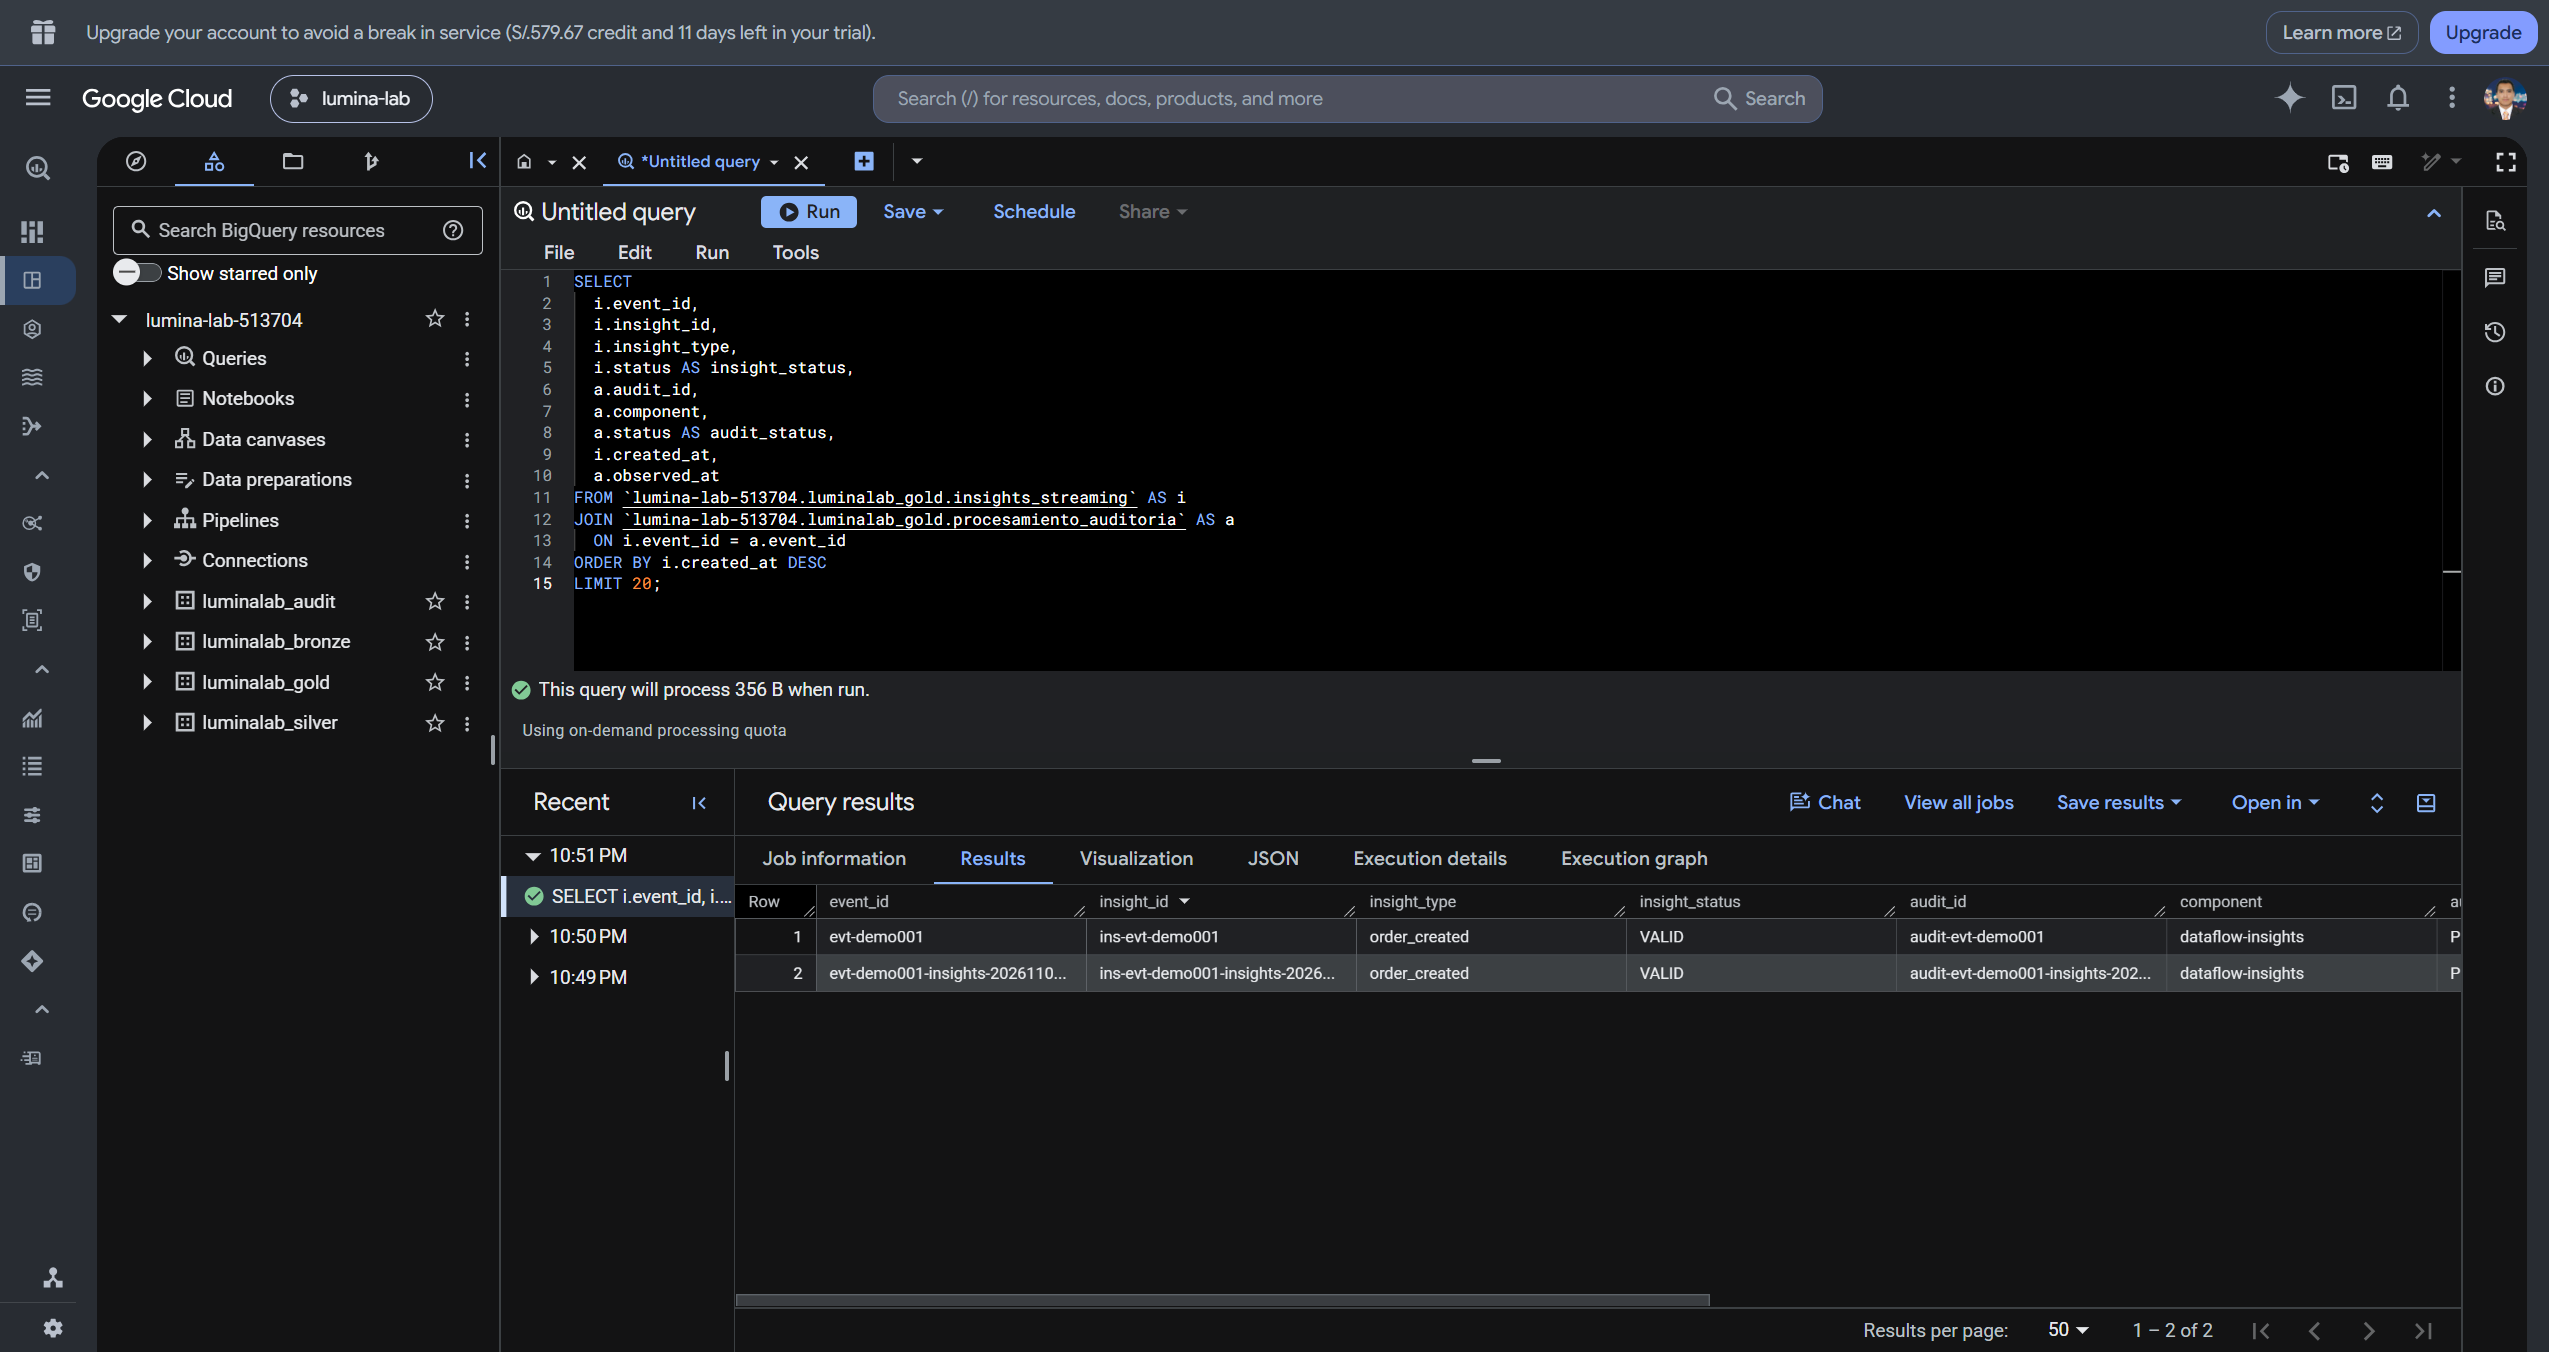
\includegraphics[width=0.96\textwidth]{../assets/evidencia/03-insights/01-bq-insights-auditoria.png}
\caption{Vista de Insights y auditoría}
\end{figure}






\clearpage
\section{Implementación de pipelines batch}

\begin{center}

\includegraphics[width=.4704\textwidth]{../assets/miniportadas/06-batch.png}
\end{center}

\subsection{Recorrido de procesamiento por lotes}

La app batch genera JSONL por dominio en Cloud Storage Landing, carga cada archivo a una tabla de staging de BigQuery y hace MERGE a Bronze (*\_raw). Al finalizar la generación, solicita una ejecución de Workflows; este ejecuta SQL en BigQuery para curar seis dominios Silver y materializar CU01-CU03 y operational\_\allowbreak{}mart. La solicitud es asíncrona: el estado de la app confirma la carga Bronze y el inicio, no la finalización de Gold.\par

\begingroup\small
\begin{longtable}{@{}>{\raggedright\arraybackslash}p{0.2268\textwidth}>{\raggedright\arraybackslash}p{0.2268\textwidth}>{\raggedright\arraybackslash}p{0.2268\textwidth}>{\raggedright\arraybackslash}p{0.2268\textwidth}@{}}
\toprule
\textbf{Dominio} & \textbf{Tabla Bronze} & \textbf{Tabla Silver} & \textbf{Clave de negocio declarada} \\
\midrule
\endfirsthead
\toprule
\textbf{Dominio} & \textbf{Tabla Bronze} & \textbf{Tabla Silver} & \textbf{Clave de negocio declarada} \\
\midrule
\endhead
Pedidos & pedidos\_\allowbreak{}raw & pedidos & order\_\allowbreak{}id + order\_\allowbreak{}line\_\allowbreak{}id \\
Inventario & inventario\_\allowbreak{}raw & inventario & snapshot\_\allowbreak{}id \\
Entregas & entregas\_\allowbreak{}raw & entregas & delivery\_\allowbreak{}id \\
Competidores & benchmark\_\allowbreak{}competidores\_\allowbreak{}raw & benchmark\_\allowbreak{}competidores & benchmark\_\allowbreak{}id \\
Eventos locales & eventos\_\allowbreak{}locales\_\allowbreak{}raw & eventos\_\allowbreak{}locales & local\_\allowbreak{}event\_\allowbreak{}id \\
Redes sociales & redes\_\allowbreak{}sociales\_\allowbreak{}raw & redes\_\allowbreak{}sociales & post\_\allowbreak{}id \\
\bottomrule
\end{longtable}
\endgroup

\subsection{Contrato de ejecución de lote}

\begingroup\small
\begin{longtable}{@{}>{\raggedright\arraybackslash}p{0.2268\textwidth}>{\raggedright\arraybackslash}p{0.2268\textwidth}>{\raggedright\arraybackslash}p{0.2268\textwidth}>{\raggedright\arraybackslash}p{0.2268\textwidth}@{}}
\toprule
\textbf{Etapa} & \textbf{Entrada} & \textbf{Procesamiento} & \textbf{Salida y control} \\
\midrule
\endfirsthead
\toprule
\textbf{Etapa} & \textbf{Entrada} & \textbf{Procesamiento} & \textbf{Salida y control} \\
\midrule
\endhead
Identificación & archivo ad hoc & asignar batch\_\allowbreak{}id, file\_\allowbreak{}id y record\_\allowbreak{}hash & referencia reproducible de archivo \\
Ingesta & archivo de Landing & cargar JSON y procedencia & Bronze.*\_\allowbreak{}raw con payload\_\allowbreak{}json e is\_\allowbreak{}valid \\
Curación & Bronze.*\_\allowbreak{}raw filtrado por batch\_\allowbreak{}id & JSON\_\allowbreak{}VALUE, SAFE\_\allowbreak{}CAST, MERGE & seis entidades Silver y quality\_\allowbreak{}status \\
Publicación & pedidos, inventario y entregas Silver & joins, cálculos y agregaciones & CU01-CU03 y operational\_\allowbreak{}mart \\
Conciliación & identificador de ejecución & comparar conteos, nulos, duplicados y estado & acta y ejecución Workflows \\
\bottomrule
\end{longtable}
\endgroup

Los campos físicos del envelope Bronze, las claves de cada dominio y los esquemas de entrada se detallan en el anexo E.\par
\textbf{Salida analítica:} pedidos + inventario alimentan CU01 y CU02; pedidos + entregas alimentan CU03. Los seis dominios aportan sus campos seleccionados al operational\_\allowbreak{}mart. Los campos completos de entrada y su proyección se detallan en los anexos E y F.\par

La ruta de la app productora no utiliza Storage Transfer ni Dataproc: escribe Landing directamente, carga Bronze con BigQuery y transforma con SQL orquestado por Workflows. Los scripts de Storage Transfer y el job Dataproc son rutas separadas del repositorio; no forman parte de este recorrido E2E.\par


\begin{figure}[htbp]
\centering
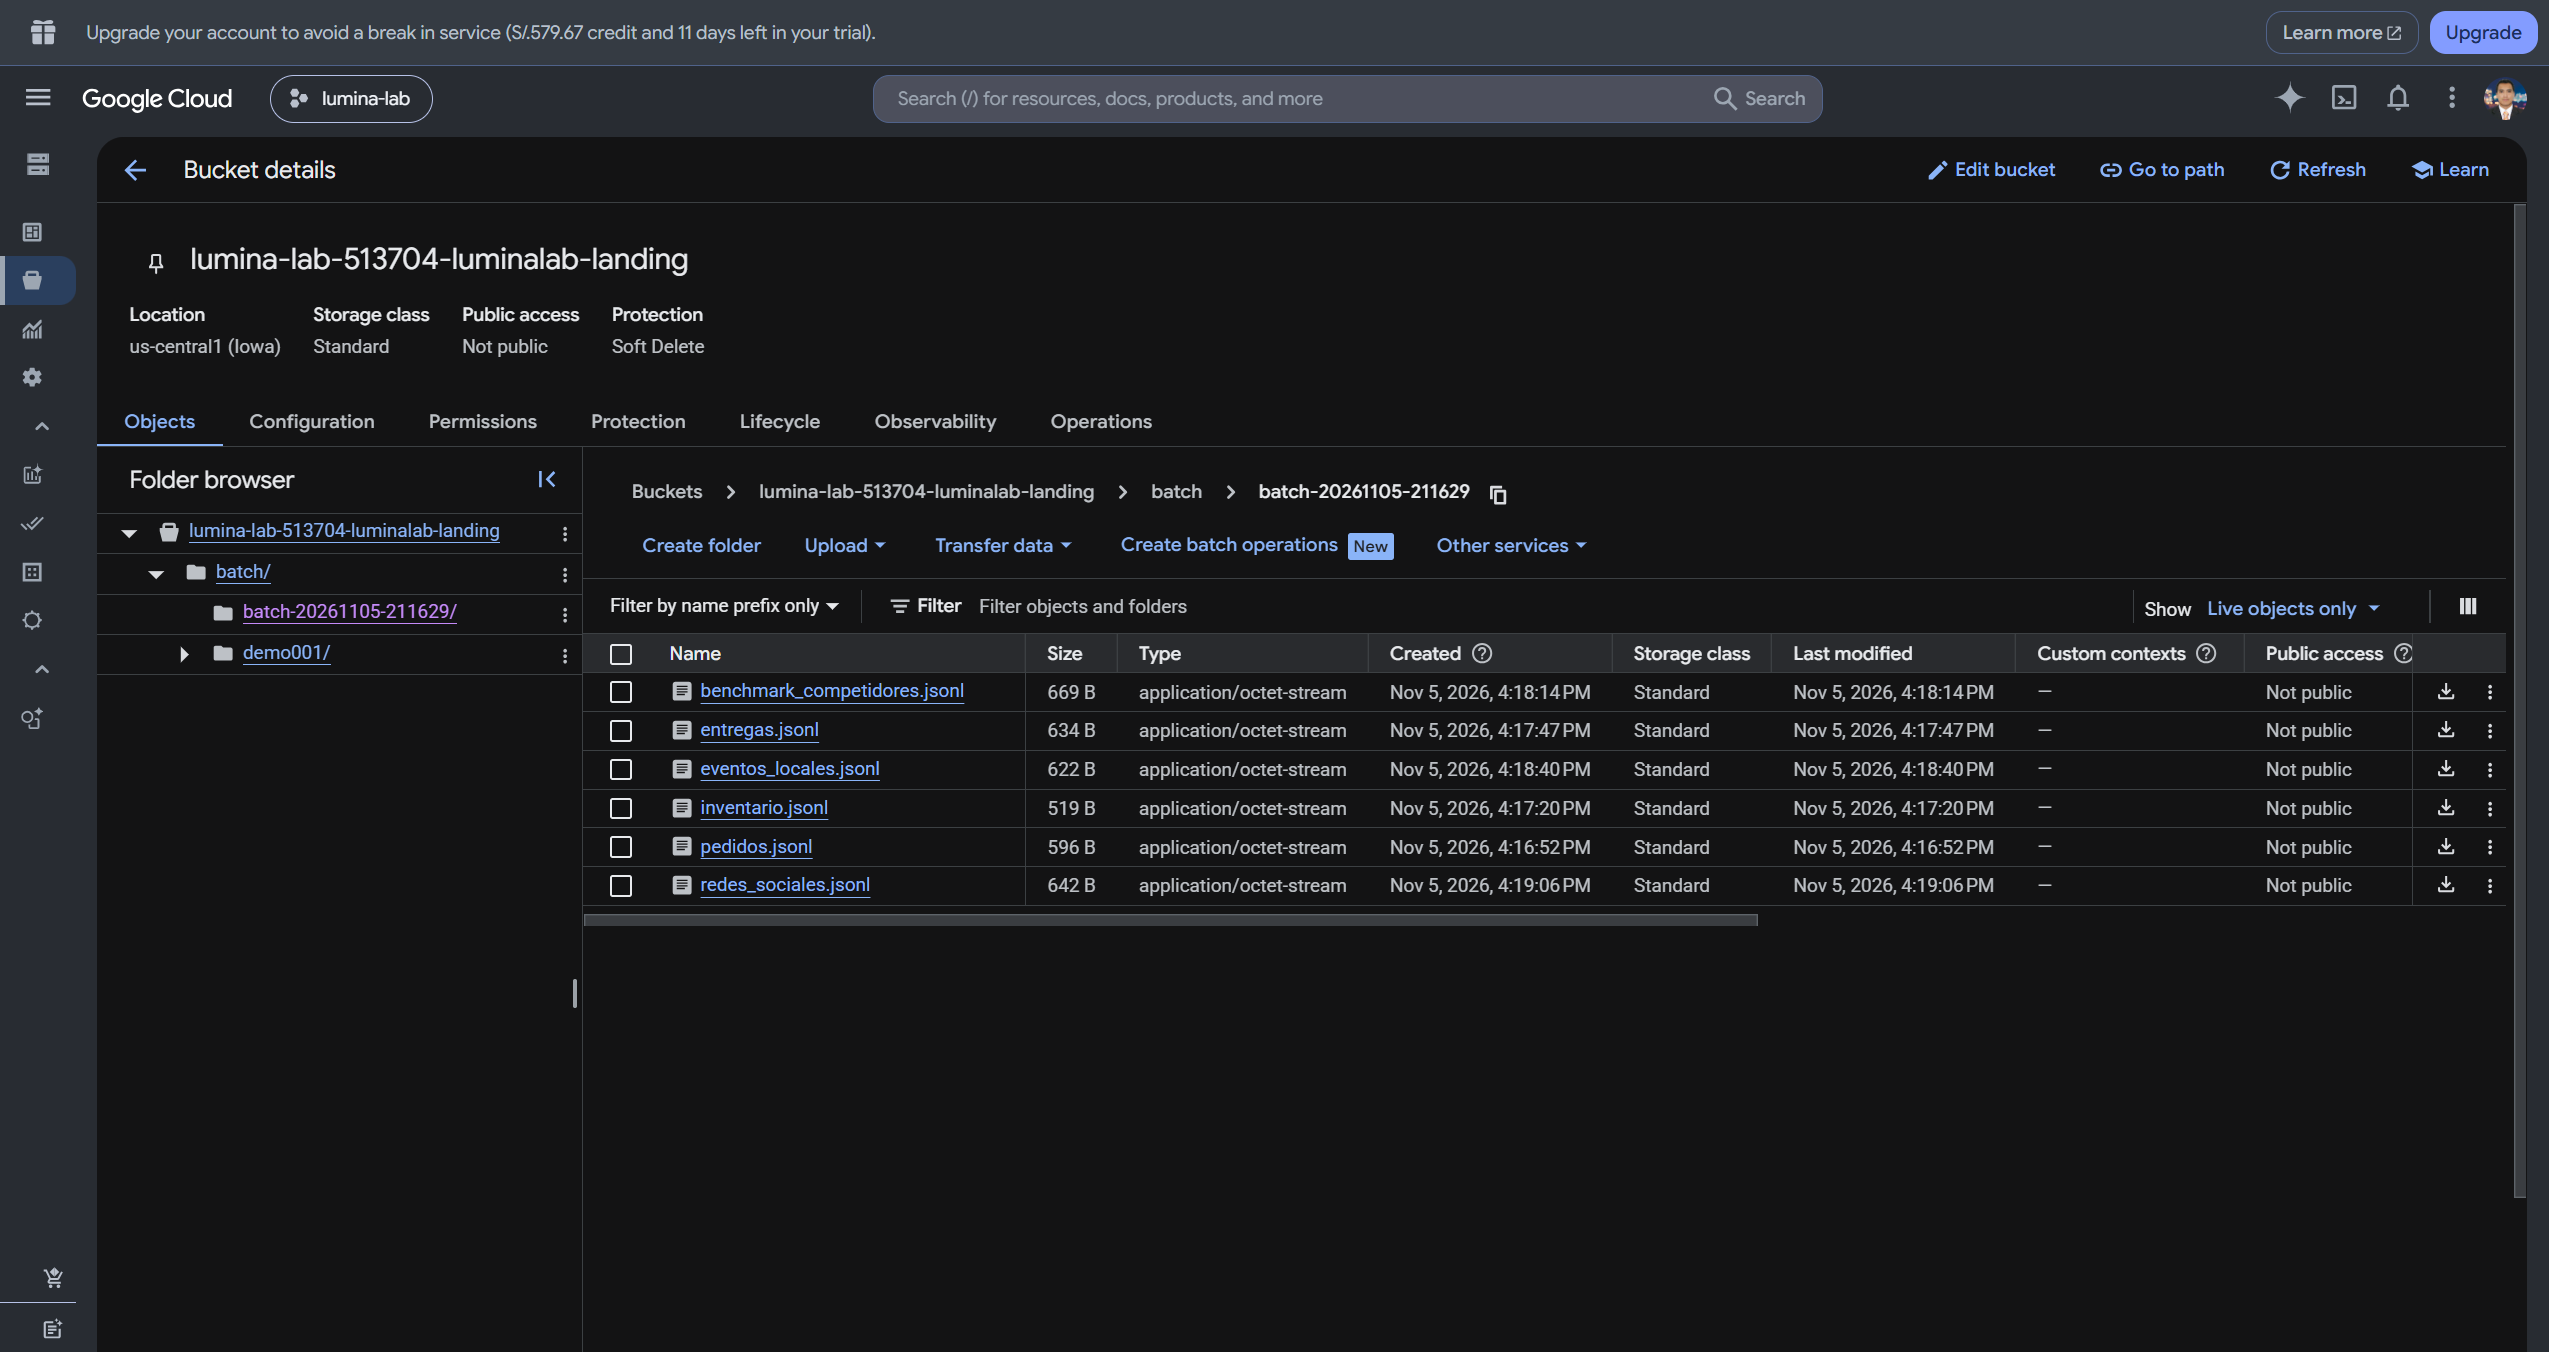
\includegraphics[width=0.96\textwidth]{../assets/evidencia/04-batch/01-landing-transfer.png}
\caption{Vista de Landing y transferencia}
\end{figure}



\begin{figure}[htbp]
\centering
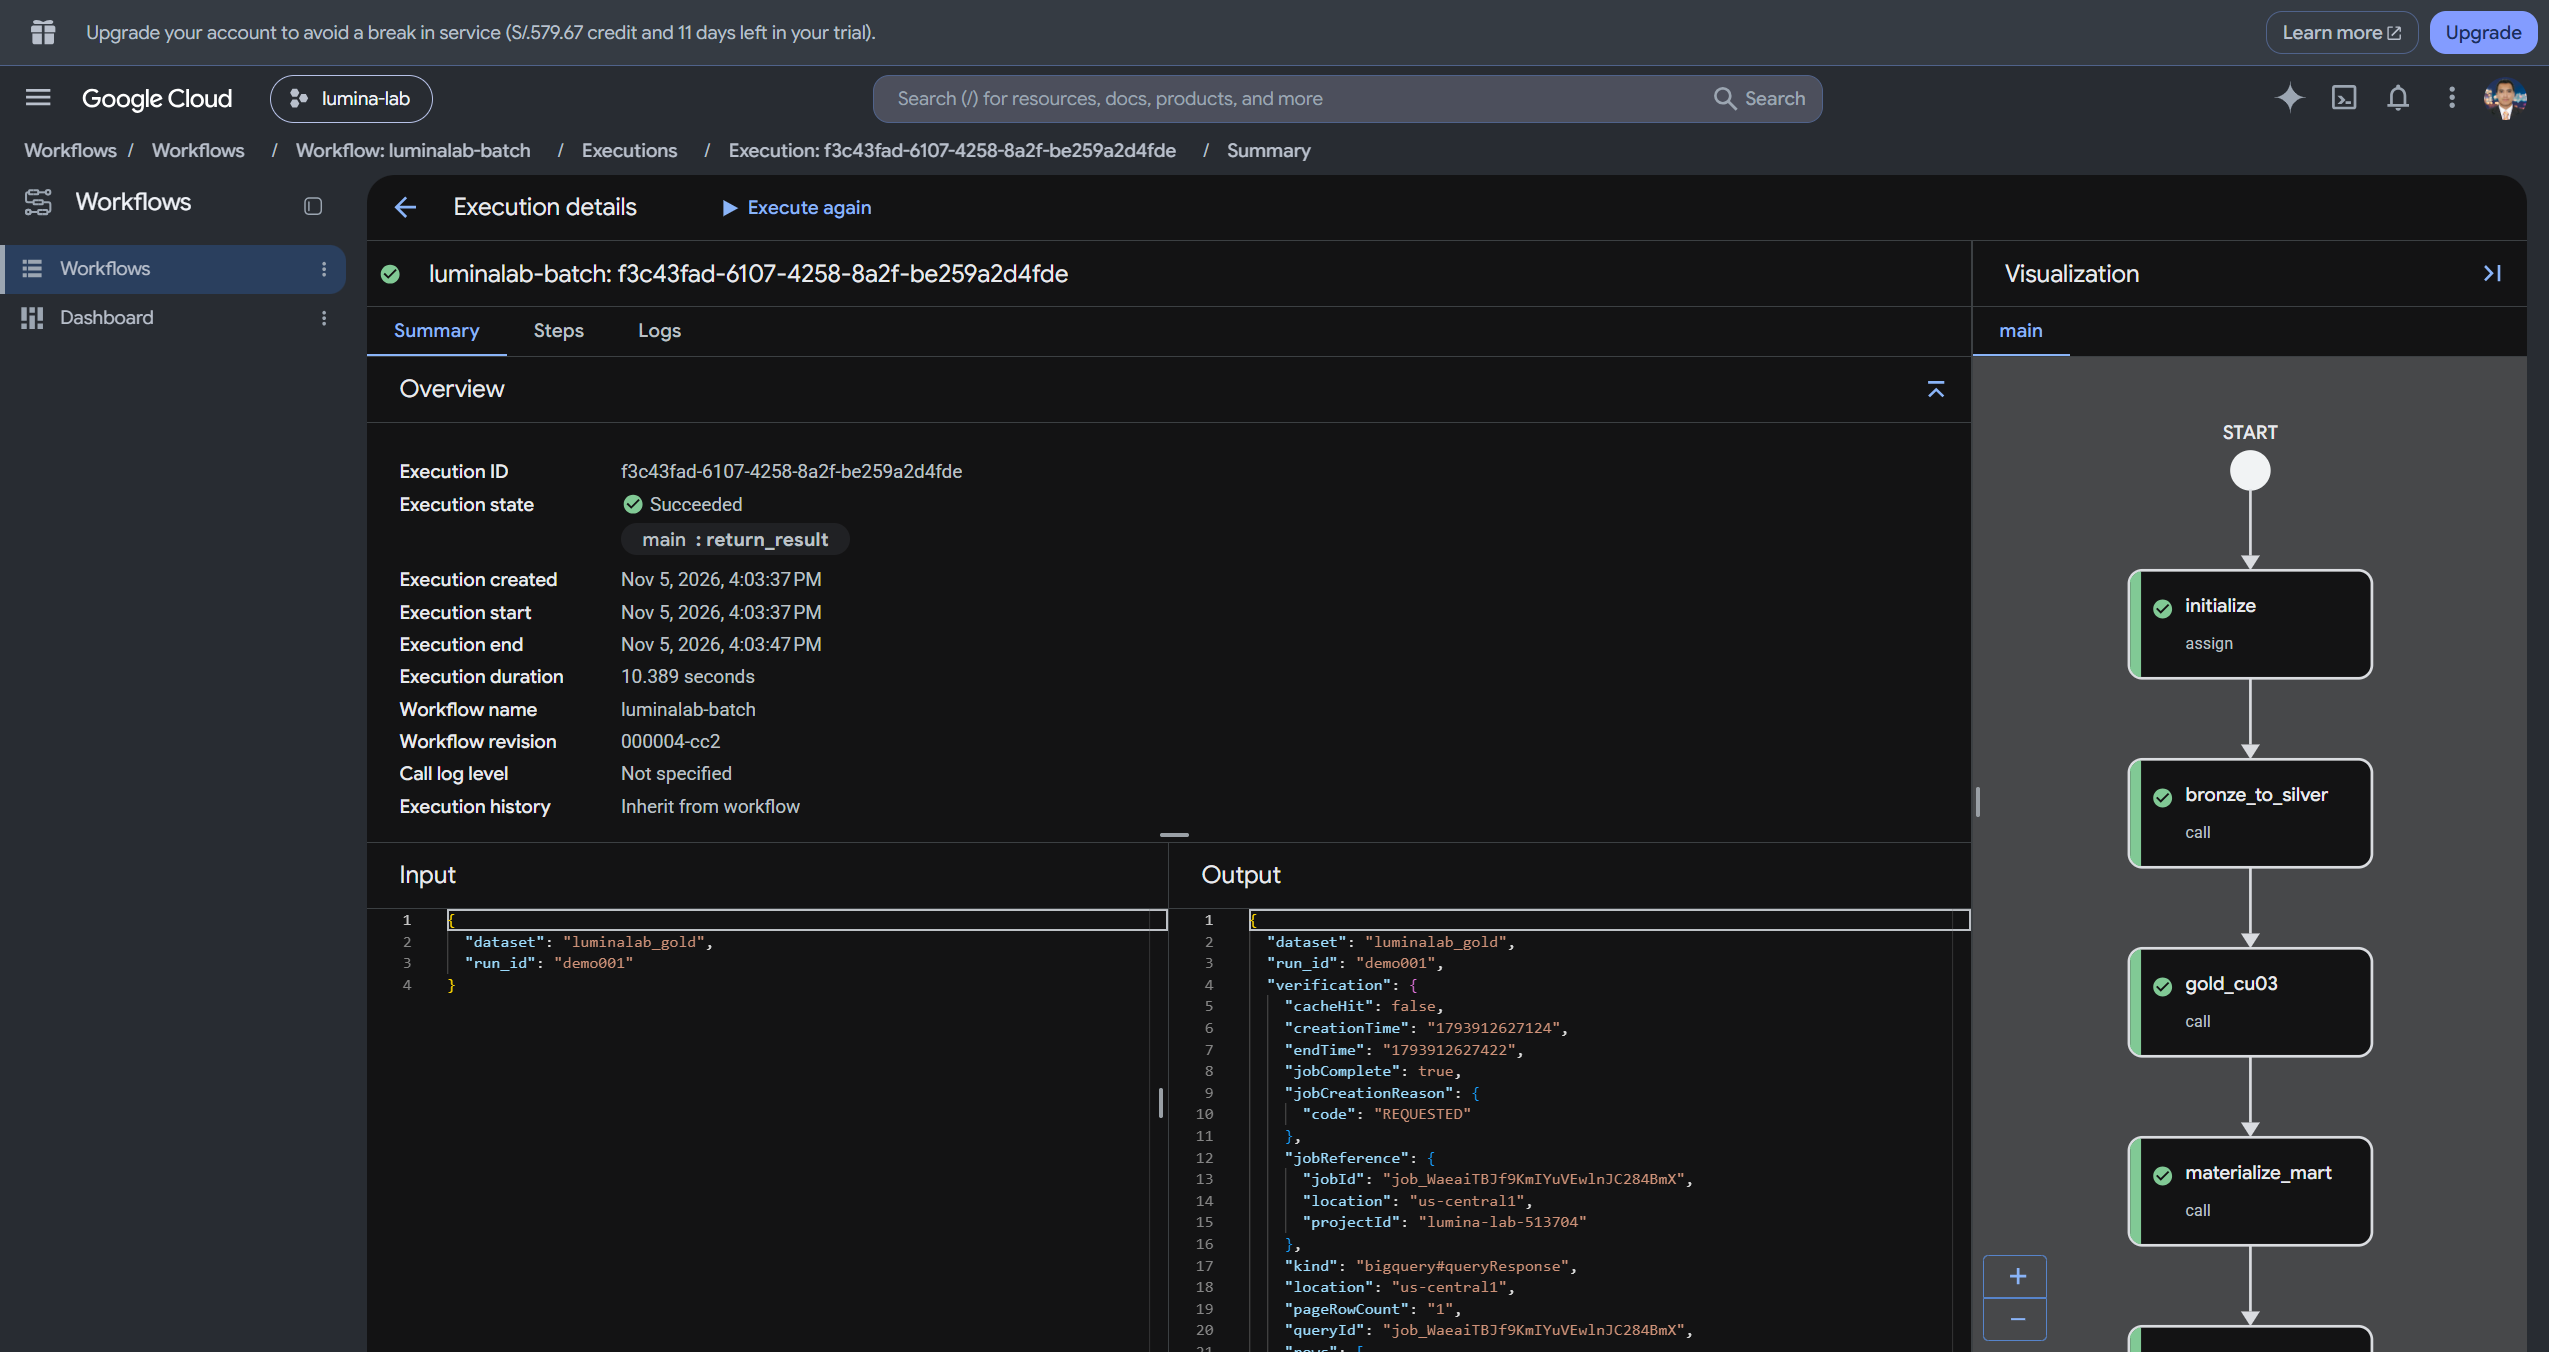
\includegraphics[width=0.96\textwidth]{../assets/evidencia/04-batch/02-workflow-execution.png}
\caption{Vista de Ejecución Workflows}
\end{figure}



\begin{figure}[htbp]
\centering
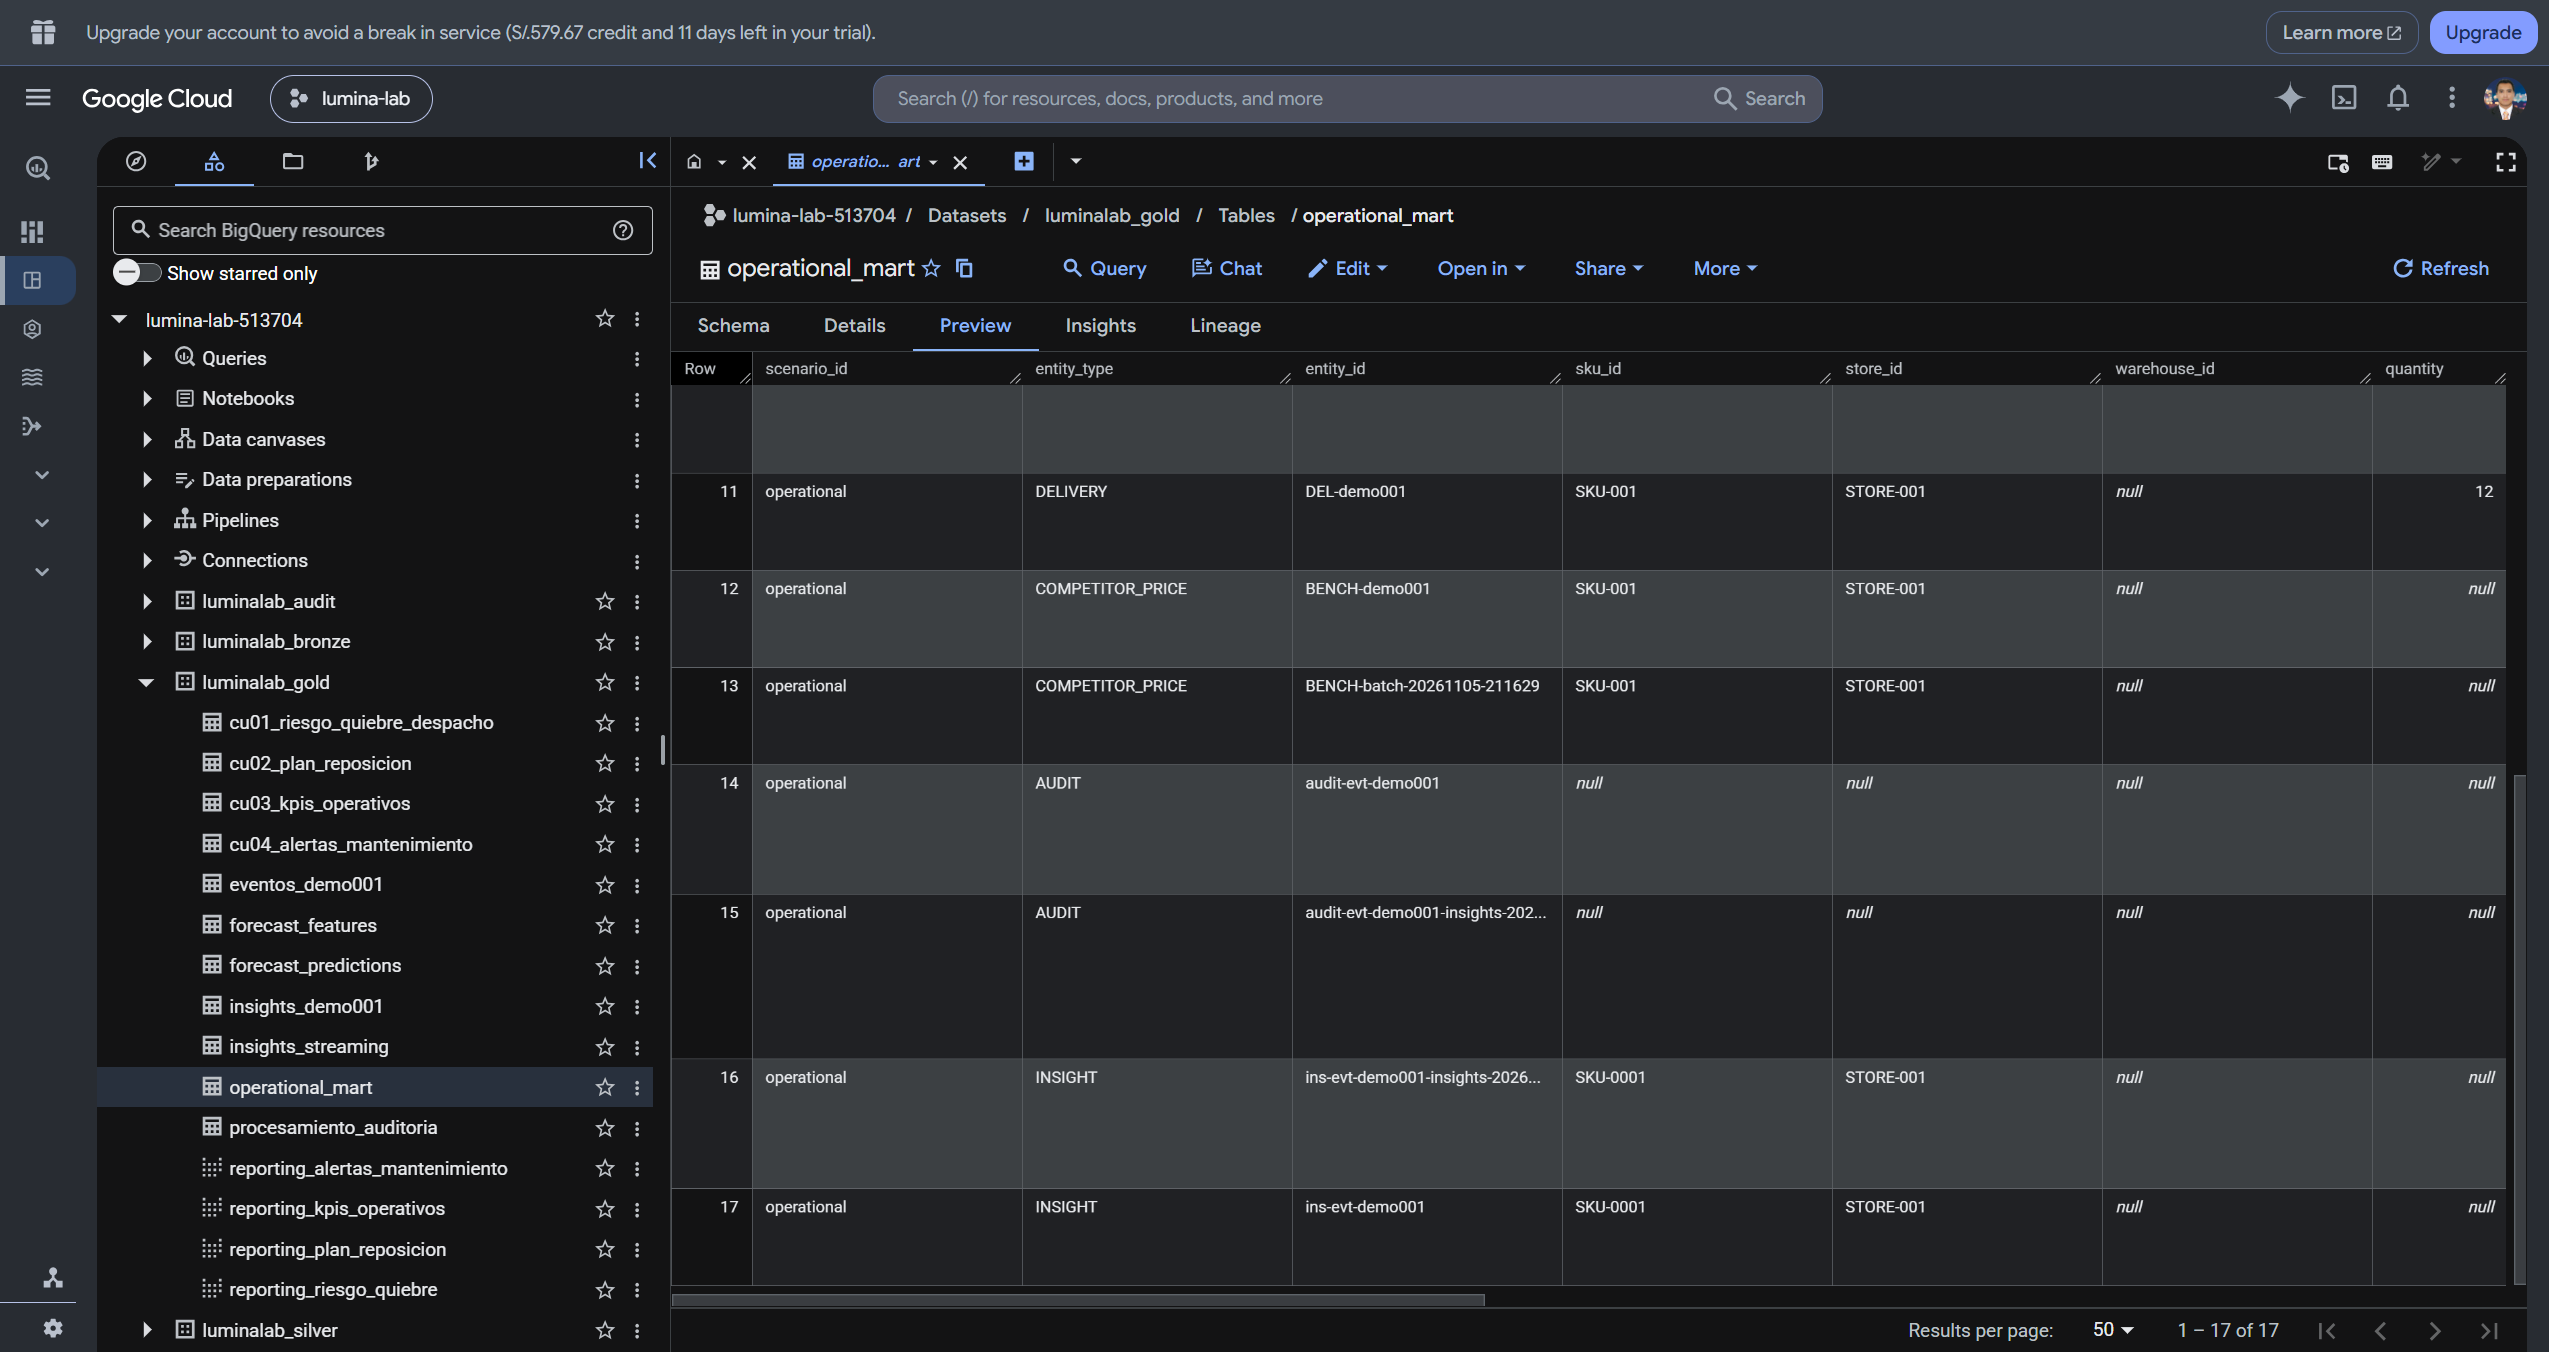
\includegraphics[width=0.96\textwidth]{../assets/evidencia/04-batch/03-bq-batch-mart.png}
\caption{Vista de Recorrido batch a Mart}
\end{figure}






\clearpage
\section{Transformación, calidad e integración}

\begin{center}

\includegraphics[width=.4704\textwidth]{../assets/miniportadas/07-transformacion-calidad.png}
\end{center}

\subsection{Reglas de transformación verificables}

\begingroup\small
\begin{longtable}{@{}>{\raggedright\arraybackslash}p{0.2268\textwidth}>{\raggedright\arraybackslash}p{0.2268\textwidth}>{\raggedright\arraybackslash}p{0.2268\textwidth}>{\raggedright\arraybackslash}p{0.2268\textwidth}@{}}
\toprule
\textbf{Regla} & \textbf{Ejemplo de entrada} & \textbf{Salida esperada} & \textbf{Comprobación} \\
\midrule
\endfirsthead
\toprule
\textbf{Regla} & \textbf{Ejemplo de entrada} & \textbf{Salida esperada} & \textbf{Comprobación} \\
\midrule
\endhead
Tipado & cantidad como texto & cantidad numérica o rechazo & tipo físico y error \\
Normalización & identificador con espacios & clave canónica & comparación origen/\allowbreak{}destino \\
Integridad & pedido sin identificador & registro rechazado o marcado & conteo por calidad \\
Duplicidad & mismo event\_\allowbreak{}id repetido & efecto controlado & consulta por event\_\allowbreak{}id \\
Temporalidad & evento tardío & vigencia registrada & occurred\_\allowbreak{}at vs emitted\_\allowbreak{}at \\
Enriquecimiento & SKU y ubicación válidos & atributos asociados & join sustentado \\
Agregación & múltiples líneas por pedido & métrica a grano declarado & conciliación de importes \\
\bottomrule
\end{longtable}
\endgroup

Las reglas de calidad se trazan a su transformación SQL o función de procesamiento, junto con la prueba y el resultado registrado.\par

\subsection{Integración de dominios ad hoc}

Los cruces entre pedidos, inventario, entregas y datos contextuales se realizan exclusivamente con claves y correspondencias definidas por los generadores propios. Se preservan la versión del escenario, la trazabilidad del lote o evento y la granularidad de cada entidad. Antes de relacionar ventas con múltiples eventos, los registros se agregan al grano compatible para evitar multiplicar unidades o importes.\par

\subsection{Indicadores de calidad}

\begingroup\small
\begin{longtable}{@{}>{\raggedright\arraybackslash}p{0.3068\textwidth}>{\raggedright\arraybackslash}p{0.3068\textwidth}>{\raggedright\arraybackslash}p{0.3068\textwidth}@{}}
\toprule
\textbf{Métrica} & \textbf{Fórmula} & \textbf{Interpretación} \\
\midrule
\endfirsthead
\toprule
\textbf{Métrica} & \textbf{Fórmula} & \textbf{Interpretación} \\
\midrule
\endhead
Completitud & campos obligatorios presentes / filas recibidas & calidad de origen \\
Duplicidad & claves repetidas / filas recibidas & idempotencia y control \\
Rechazos & filas inválidas / filas recibidas & incumplimiento contractual \\
Conciliación & filas aceptadas + rechazadas vs recibidas & integridad del lote \\
Oportunidad & tiempo de disponibilidad - occurred\_\allowbreak{}at & latencia real \\
\bottomrule
\end{longtable}
\endgroup

\textbf{Prueba de integración:} registrar para al menos un evento y un lote las entradas, reglas, salidas y consultas antes/\allowbreak{}después, junto con el identificador de ejecución. Los porcentajes de desempeño se presentan únicamente cuando cuentan con medición reproducible.\par




\clearpage
\section{Modelado analítico y productos Gold}

\begin{center}
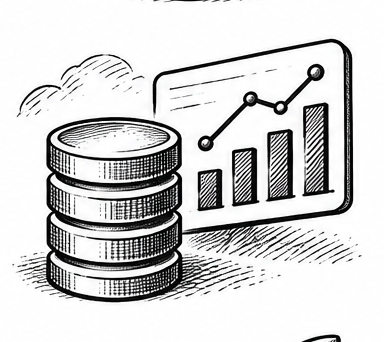
\includegraphics[width=.4704\textwidth]{../assets/miniportadas/08-modelado-gold.png}
\end{center}

\subsection{Modelo analítico y granularidad}

\begingroup\small
\begin{longtable}{@{}>{\raggedright\arraybackslash}p{0.3068\textwidth}>{\raggedright\arraybackslash}p{0.3068\textwidth}>{\raggedright\arraybackslash}p{0.3068\textwidth}@{}}
\toprule
\textbf{Producto Gold} & \textbf{Grano de consulta propuesto/\allowbreak{}documentado} & \textbf{Uso} \\
\midrule
\endfirsthead
\toprule
\textbf{Producto Gold} & \textbf{Grano de consulta propuesto/\allowbreak{}documentado} & \textbf{Uso} \\
\midrule
\endhead
cu01\_\allowbreak{}riesgo\_\allowbreak{}quiebre\_\allowbreak{}despacho & escenario, SKU y tienda & riesgo y recomendación \\
cu02\_\allowbreak{}plan\_\allowbreak{}reposicion & escenario, SKU, almacén y fecha & planificación \\
cu03\_\allowbreak{}kpis\_\allowbreak{}operativos & escenario, periodo y canal & operación y SLA \\
cu04\_\allowbreak{}alertas\_\allowbreak{}mantenimiento & escenario, activo, sensor y almacén & mantenimiento \\
operational\_\allowbreak{}mart & entity\_\allowbreak{}type, entity\_\allowbreak{}id, ingestion\_\allowbreak{}mode, source\_\allowbreak{}domain & integración transversal \\
\bottomrule
\end{longtable}
\endgroup

\textbf{Modelo dimensional:} las tablas Gold no implican automáticamente un esquema estrella; los hechos, dimensiones, claves y relaciones físicas se determinan a partir del DDL y las consultas disponibles.\par

\subsection{Forecast como capacidad complementaria}

La plataforma incluye un cálculo de referencia que transforma pedidos válidos en una estimación diaria de demanda y la incorpora al plan de reposición. El siguiente esquema muestra el recorrido y los productos generados.\par

\begin{figure}[H]
\centering
\begin{tikzpicture}[
  node distance=4mm,
  paso/.style={draw=acento,rounded corners=2pt,fill=acento!6,align=center,
    minimum height=19mm,text width=32mm,inner sep=2mm,font=\small},
  apoyo/.style={draw=acento!70,rounded corners=2pt,fill=black!3,align=center,
    minimum height=13mm,text width=50mm,inner sep=2mm,font=\small},
  flujo/.style={-{Stealth[length=2.5mm]},draw=acento,thick}]
\node[paso] (pedidos) {\textbf{Pedidos válidos}\\Silver};
\node[paso,right=of pedidos] (variables) {\textbf{Variables de demanda}\\Gold: features};
\node[paso,right=of variables] (prediccion) {\textbf{Estimación diaria}\\Gold: predicciones};
\node[paso,right=of prediccion] (plan) {\textbf{Plan de}\\\textbf{reposición}\\Gold: CU02};
\draw[flujo] (pedidos) -- (variables);
\draw[flujo] (variables) -- (prediccion);
\draw[flujo] (prediccion) -- (plan);
\node[apoyo,below=9mm of prediccion] (modelo) {\textbf{Modelo de referencia}\\Versión y metadatos\\en Cloud Storage};
\draw[flujo] (modelo) -- (prediccion);
\end{tikzpicture}
\caption{Flujo de referencia para estimación de demanda y reposición}
\end{figure}

La estimación de referencia utiliza una media móvil de siete días. No se reportan métricas de precisión predictiva.\par


\begin{figure}[htbp]
\centering
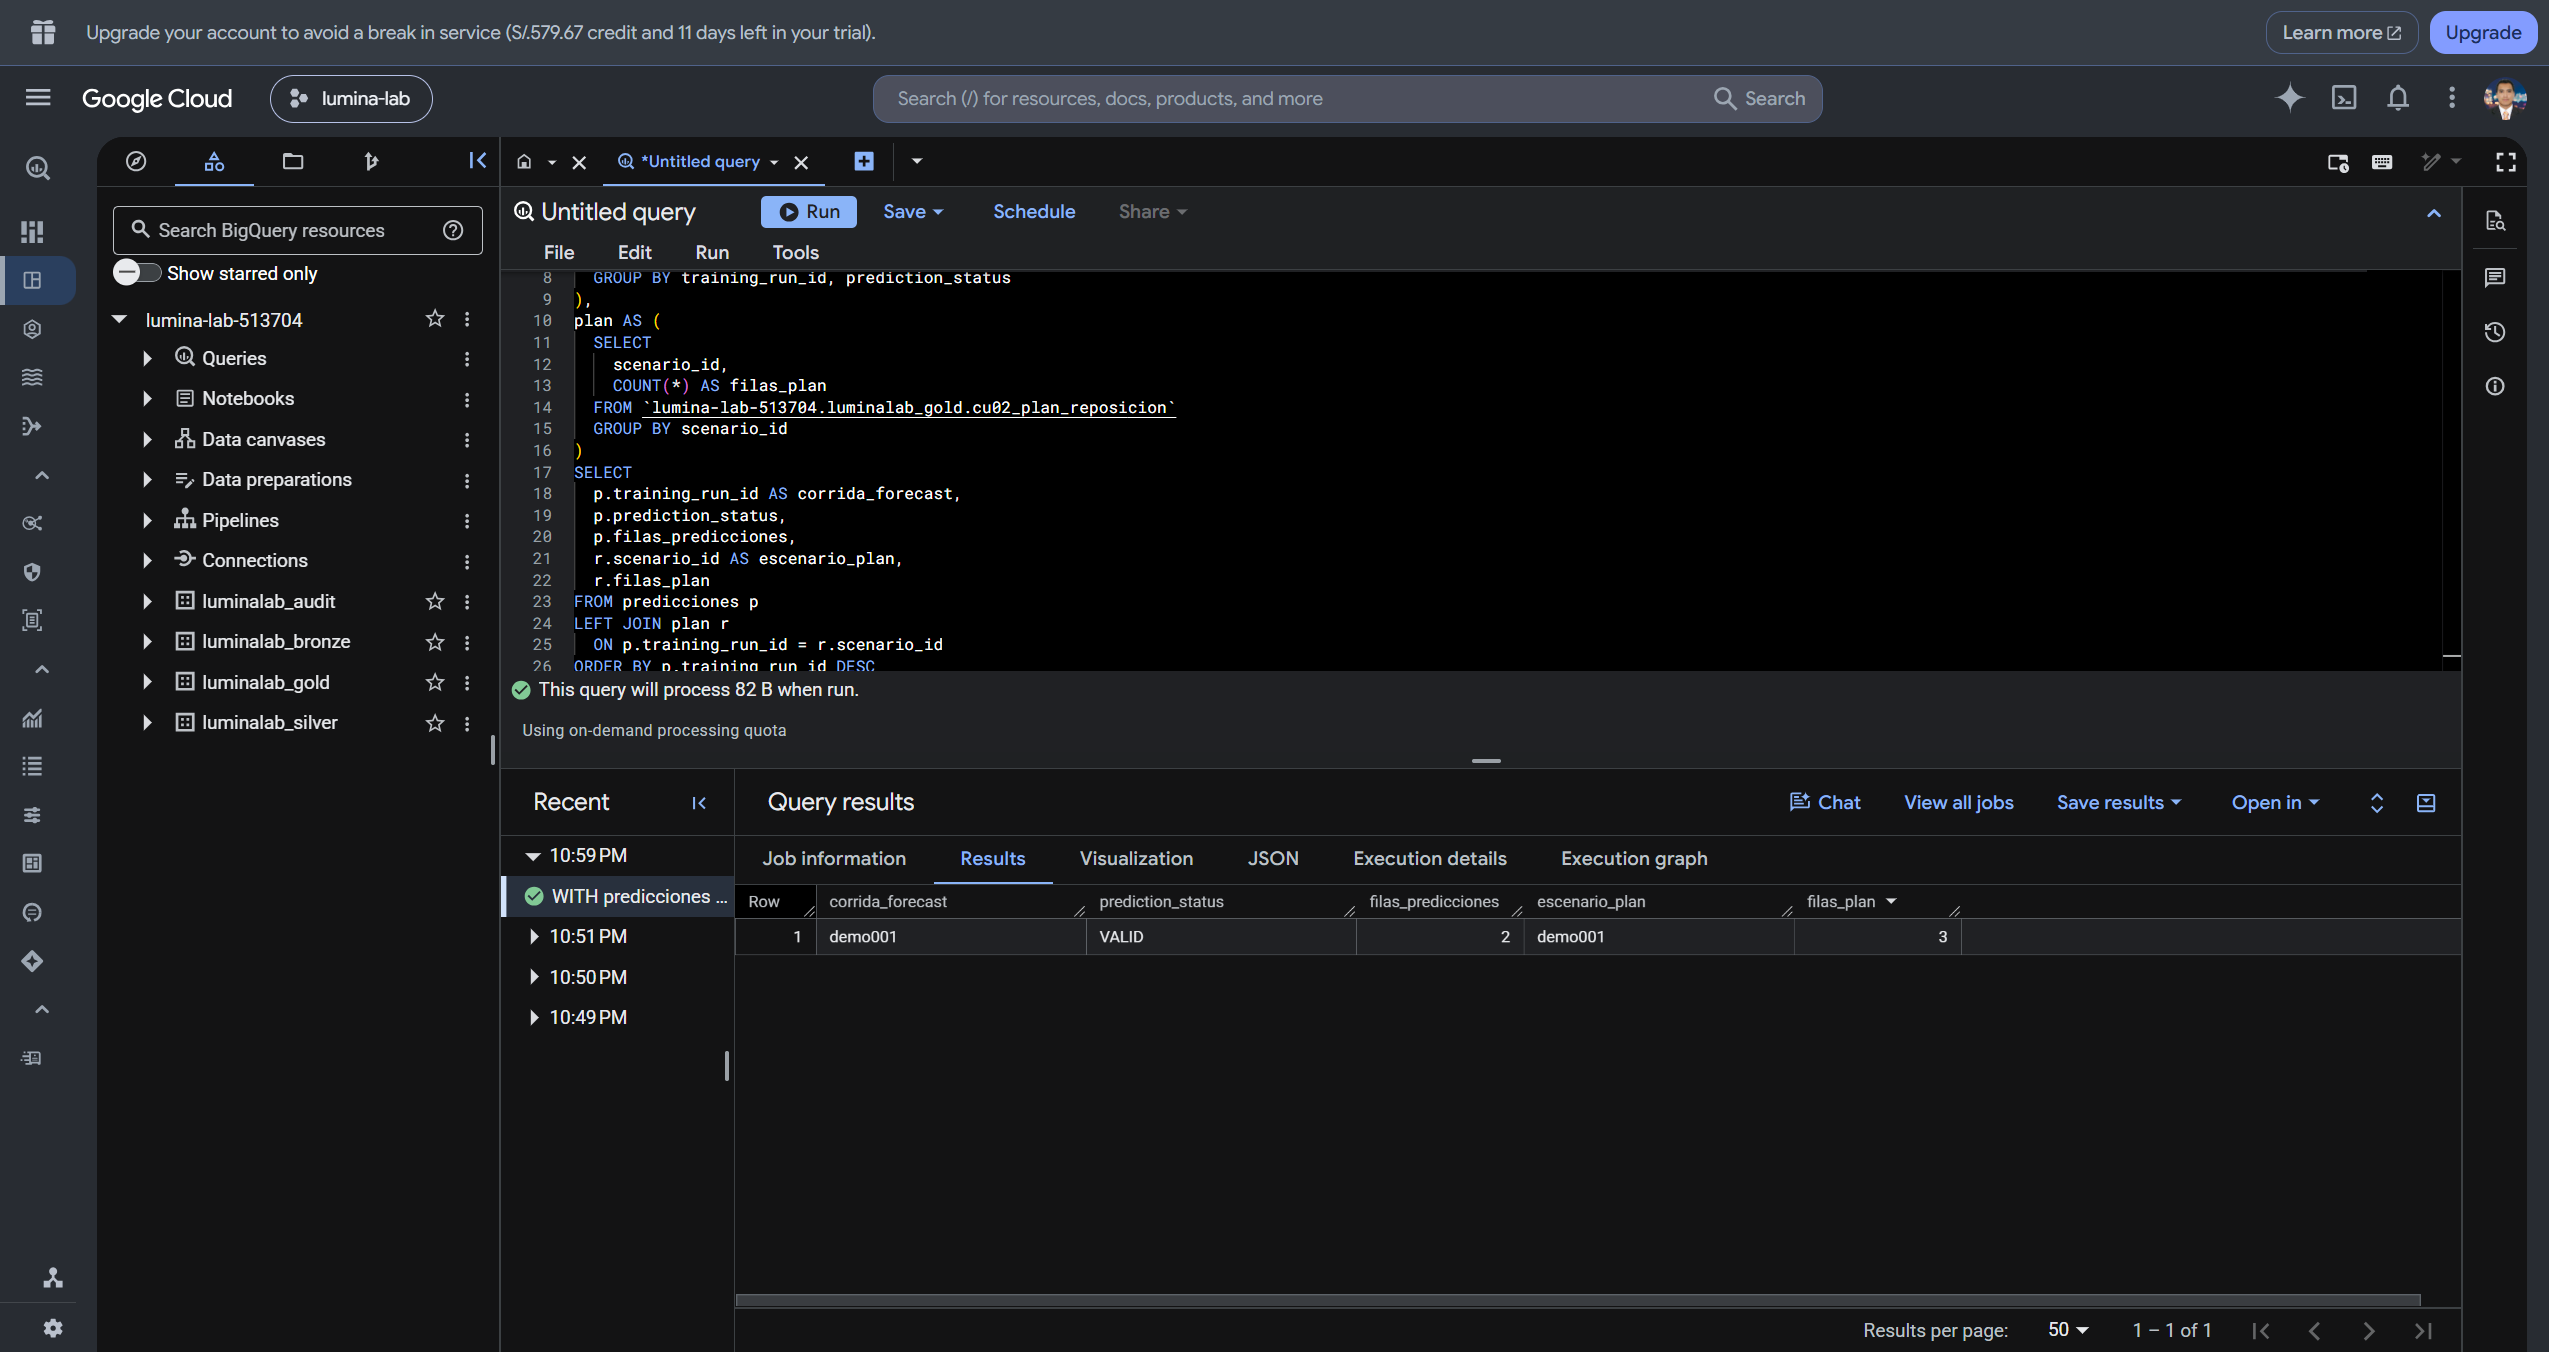
\includegraphics[width=0.96\textwidth]{../assets/evidencia/05-forecast/01-features-predicciones-plan.png}
\caption{Vista de Forecast, predicción y reposición}
\end{figure}


\subsection{Vistas de reporting}

Las vistas deben explicitar columnas, filtros, fuentes Gold y vigencia. El consumidor externo BI permanece fuera del alcance de aprovisionamiento.\par


\begin{figure}[htbp]
\centering
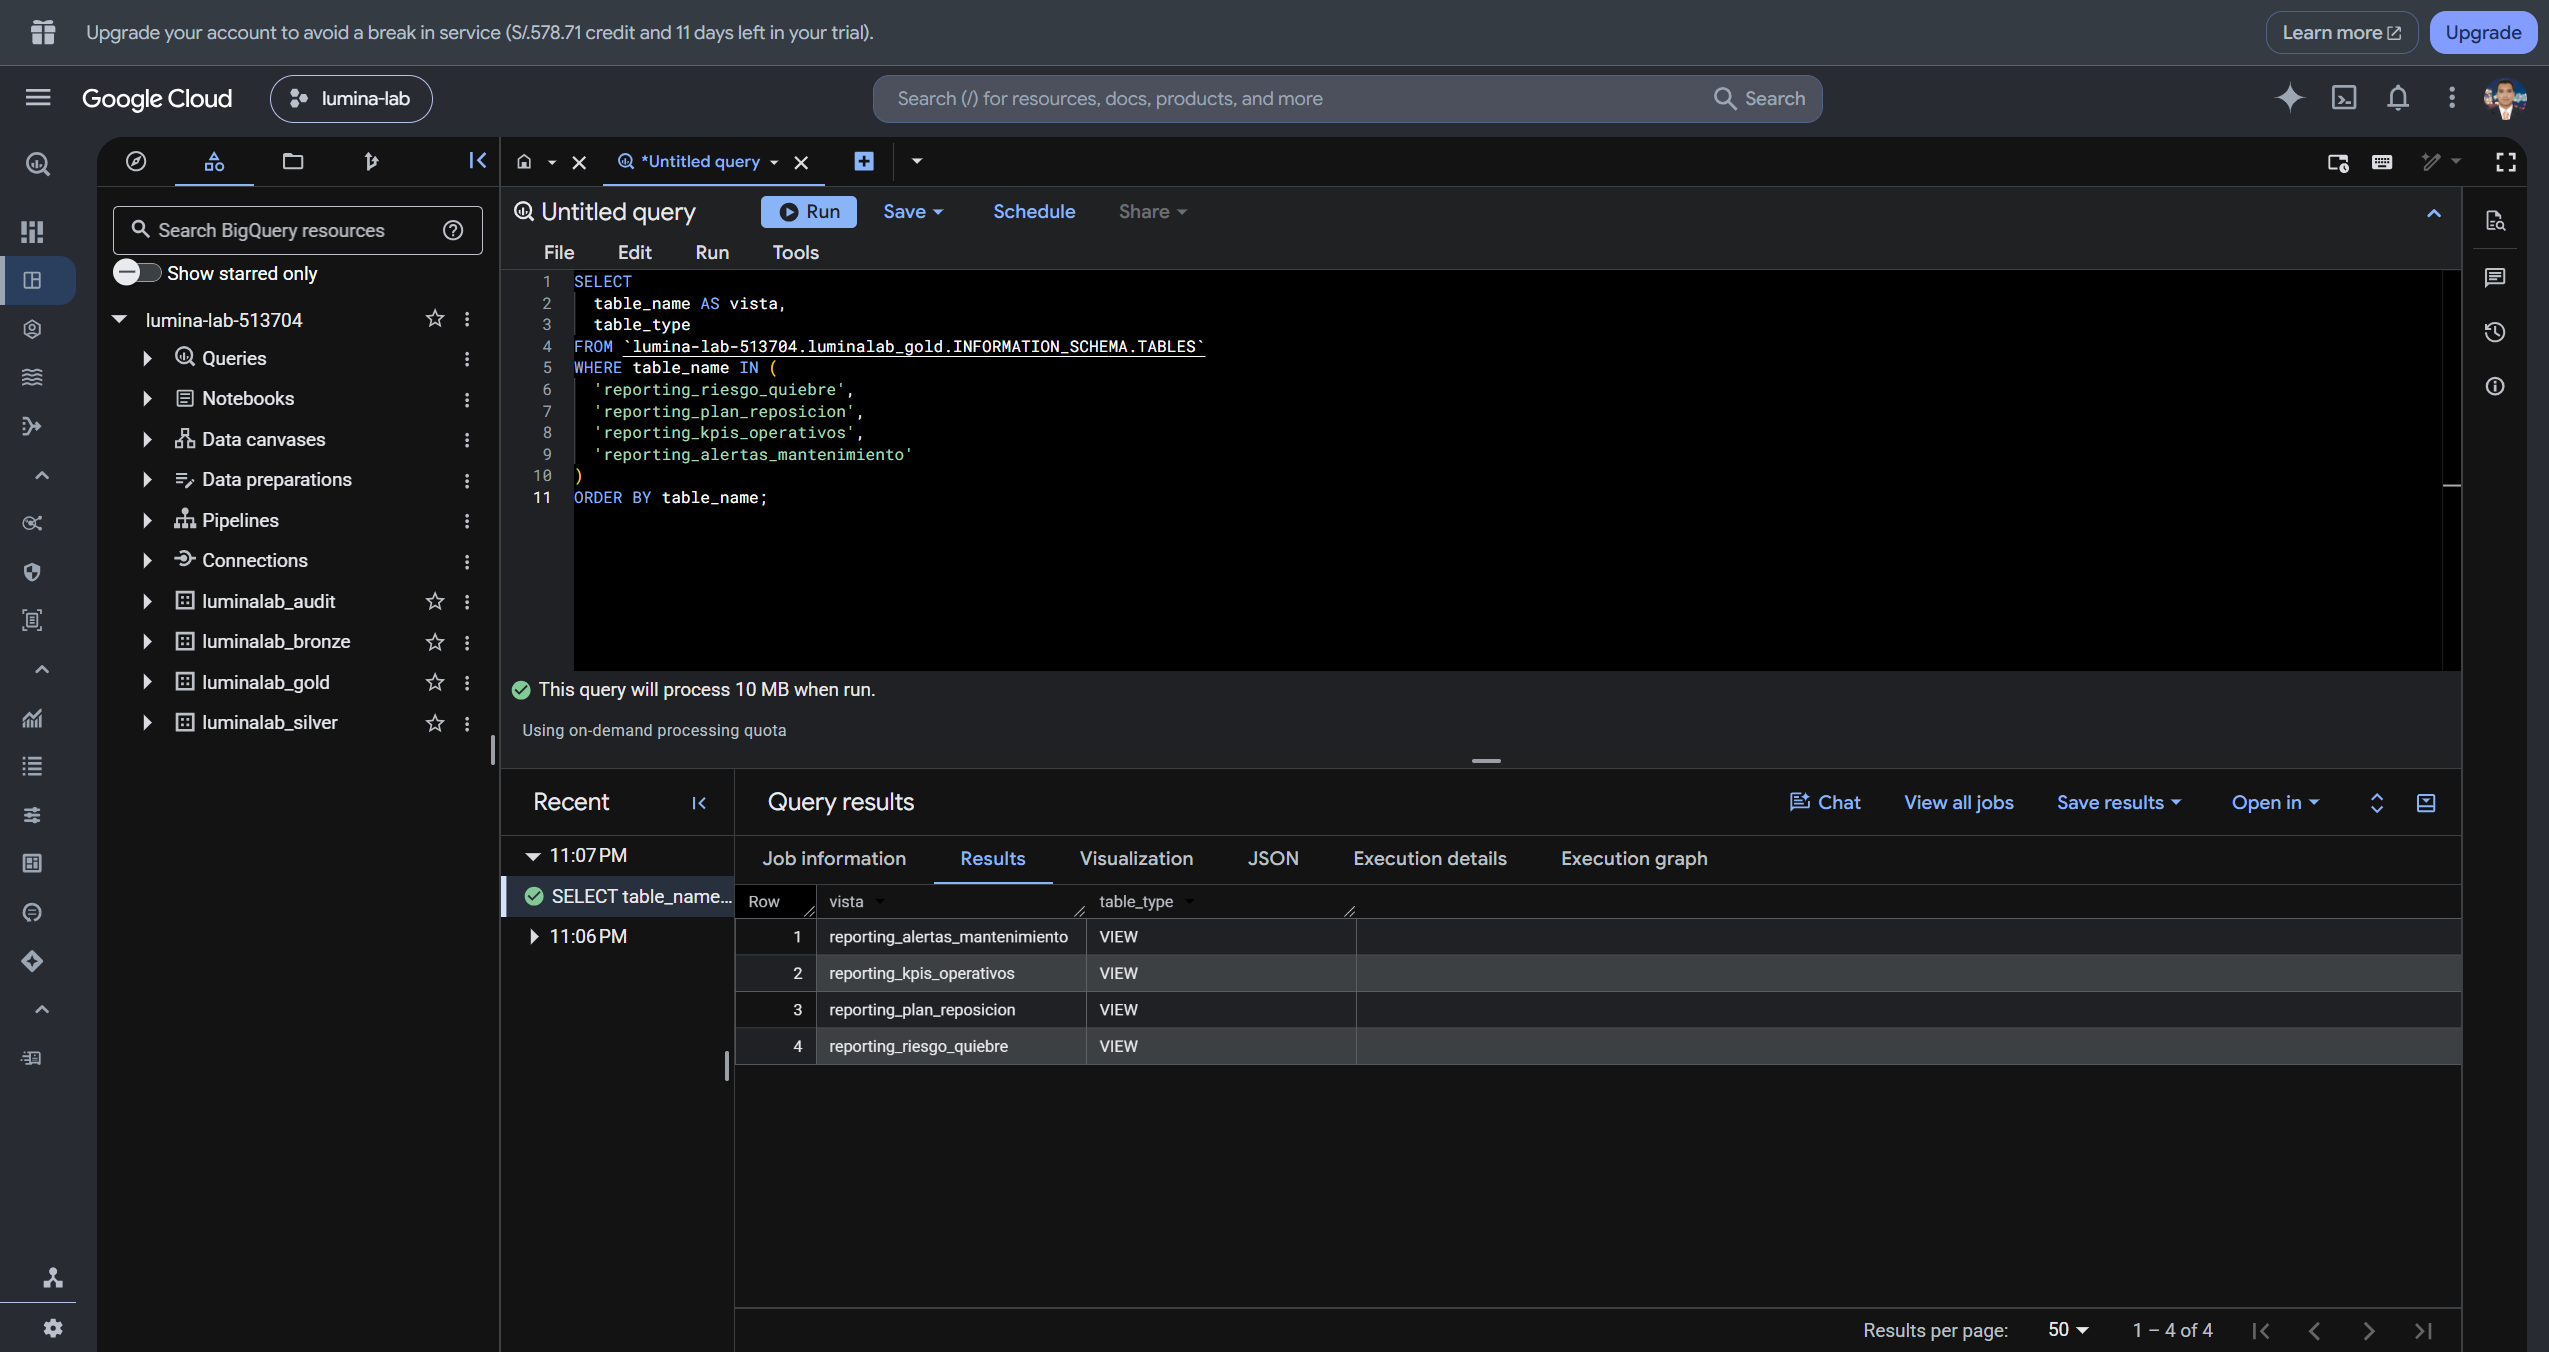
\includegraphics[width=0.96\textwidth]{../assets/evidencia/06-consumo/03-bigquery-vistas.png}
\caption{Vista de Vistas analíticas Gold}
\end{figure}






\clearpage
\section{Exposición y consumo de datos}

\begin{center}

\includegraphics[width=.4704\textwidth]{../assets/miniportadas/09-consumo-api.png}
\end{center}

\subsection{Contratos de consumo}

Cloud Run expone una API privada con autenticación IAM, mínimo cero instancias, máximo dos y límite documentado de 100 filas por solicitud. La integración con consumidores externos se gestiona mediante contratos independientes. La disponibilidad del servicio y las respuestas de negocio se verifican por separado.\par

\begingroup\small
\begin{longtable}{@{}>{\raggedright\arraybackslash}p{0.2268\textwidth}>{\raggedright\arraybackslash}p{0.2268\textwidth}>{\raggedright\arraybackslash}p{0.2268\textwidth}>{\raggedright\arraybackslash}p{0.2268\textwidth}@{}}
\toprule
\textbf{Método y ruta} & \textbf{Entrada HTTP} & \textbf{Fuente BigQuery} & \textbf{Salida JSON} \\
\midrule
\endfirsthead
\toprule
\textbf{Método y ruta} & \textbf{Entrada HTTP} & \textbf{Fuente BigQuery} & \textbf{Salida JSON} \\
\midrule
\endhead
GET /api/\allowbreak{}v1/\allowbreak{}insights & limit, scenario\_\allowbreak{}id opcional & insights\_\allowbreak{}streaming, CU01 & streaming\_\allowbreak{}insights[], stockout\_\allowbreak{}risks[], counts, scenario\_\allowbreak{}id \\
GET /api/\allowbreak{}v1/\allowbreak{}kpis & mismos parámetros & CU03 & data[], count, source\_\allowbreak{}table, scenario\_\allowbreak{}id \\
GET /api/\allowbreak{}v1/\allowbreak{}inventory-plans & mismos parámetros & CU02 & mismo envelope data[] \\
GET /api/\allowbreak{}v1/\allowbreak{}maintenance-risks & mismos parámetros & CU04 & mismo envelope data[] \\
GET /healthz & sin parámetros & ninguna & [''status'':''ok''] \\
\bottomrule
\end{longtable}
\endgroup

\begingroup\small
\begin{longtable}{@{}>{\raggedright\arraybackslash}p{0.4668\textwidth}>{\raggedright\arraybackslash}p{0.4668\textwidth}@{}}
\toprule
\textbf{Regla transversal} & \textbf{Contrato} \\
\midrule
\endfirsthead
\toprule
\textbf{Regla transversal} & \textbf{Contrato} \\
\midrule
\endhead
Autenticación & token de identidad y permiso IAM de invocación Cloud Run \\
limit & entero entre 1 y 100; valor predeterminado 25 \\
scenario\_\allowbreak{}id & cadena opcional de hasta 128 caracteres conforme al patrón definido en el anexo C \\
Errores de aplicación & HTTP 400 invalid\_\allowbreak{}query, 404 route\_\allowbreak{}not\_\allowbreak{}found, 405 method\_\allowbreak{}not\_\allowbreak{}allowed, 500 query\_\allowbreak{}failed \\
\bottomrule
\end{longtable}
\endgroup

Las respuestas y los errores se derivan de soluciones/\allowbreak{}api-insights/\allowbreak{}main.py; el anexo C presenta los contratos completos.\par


\begin{figure}[htbp]
\centering
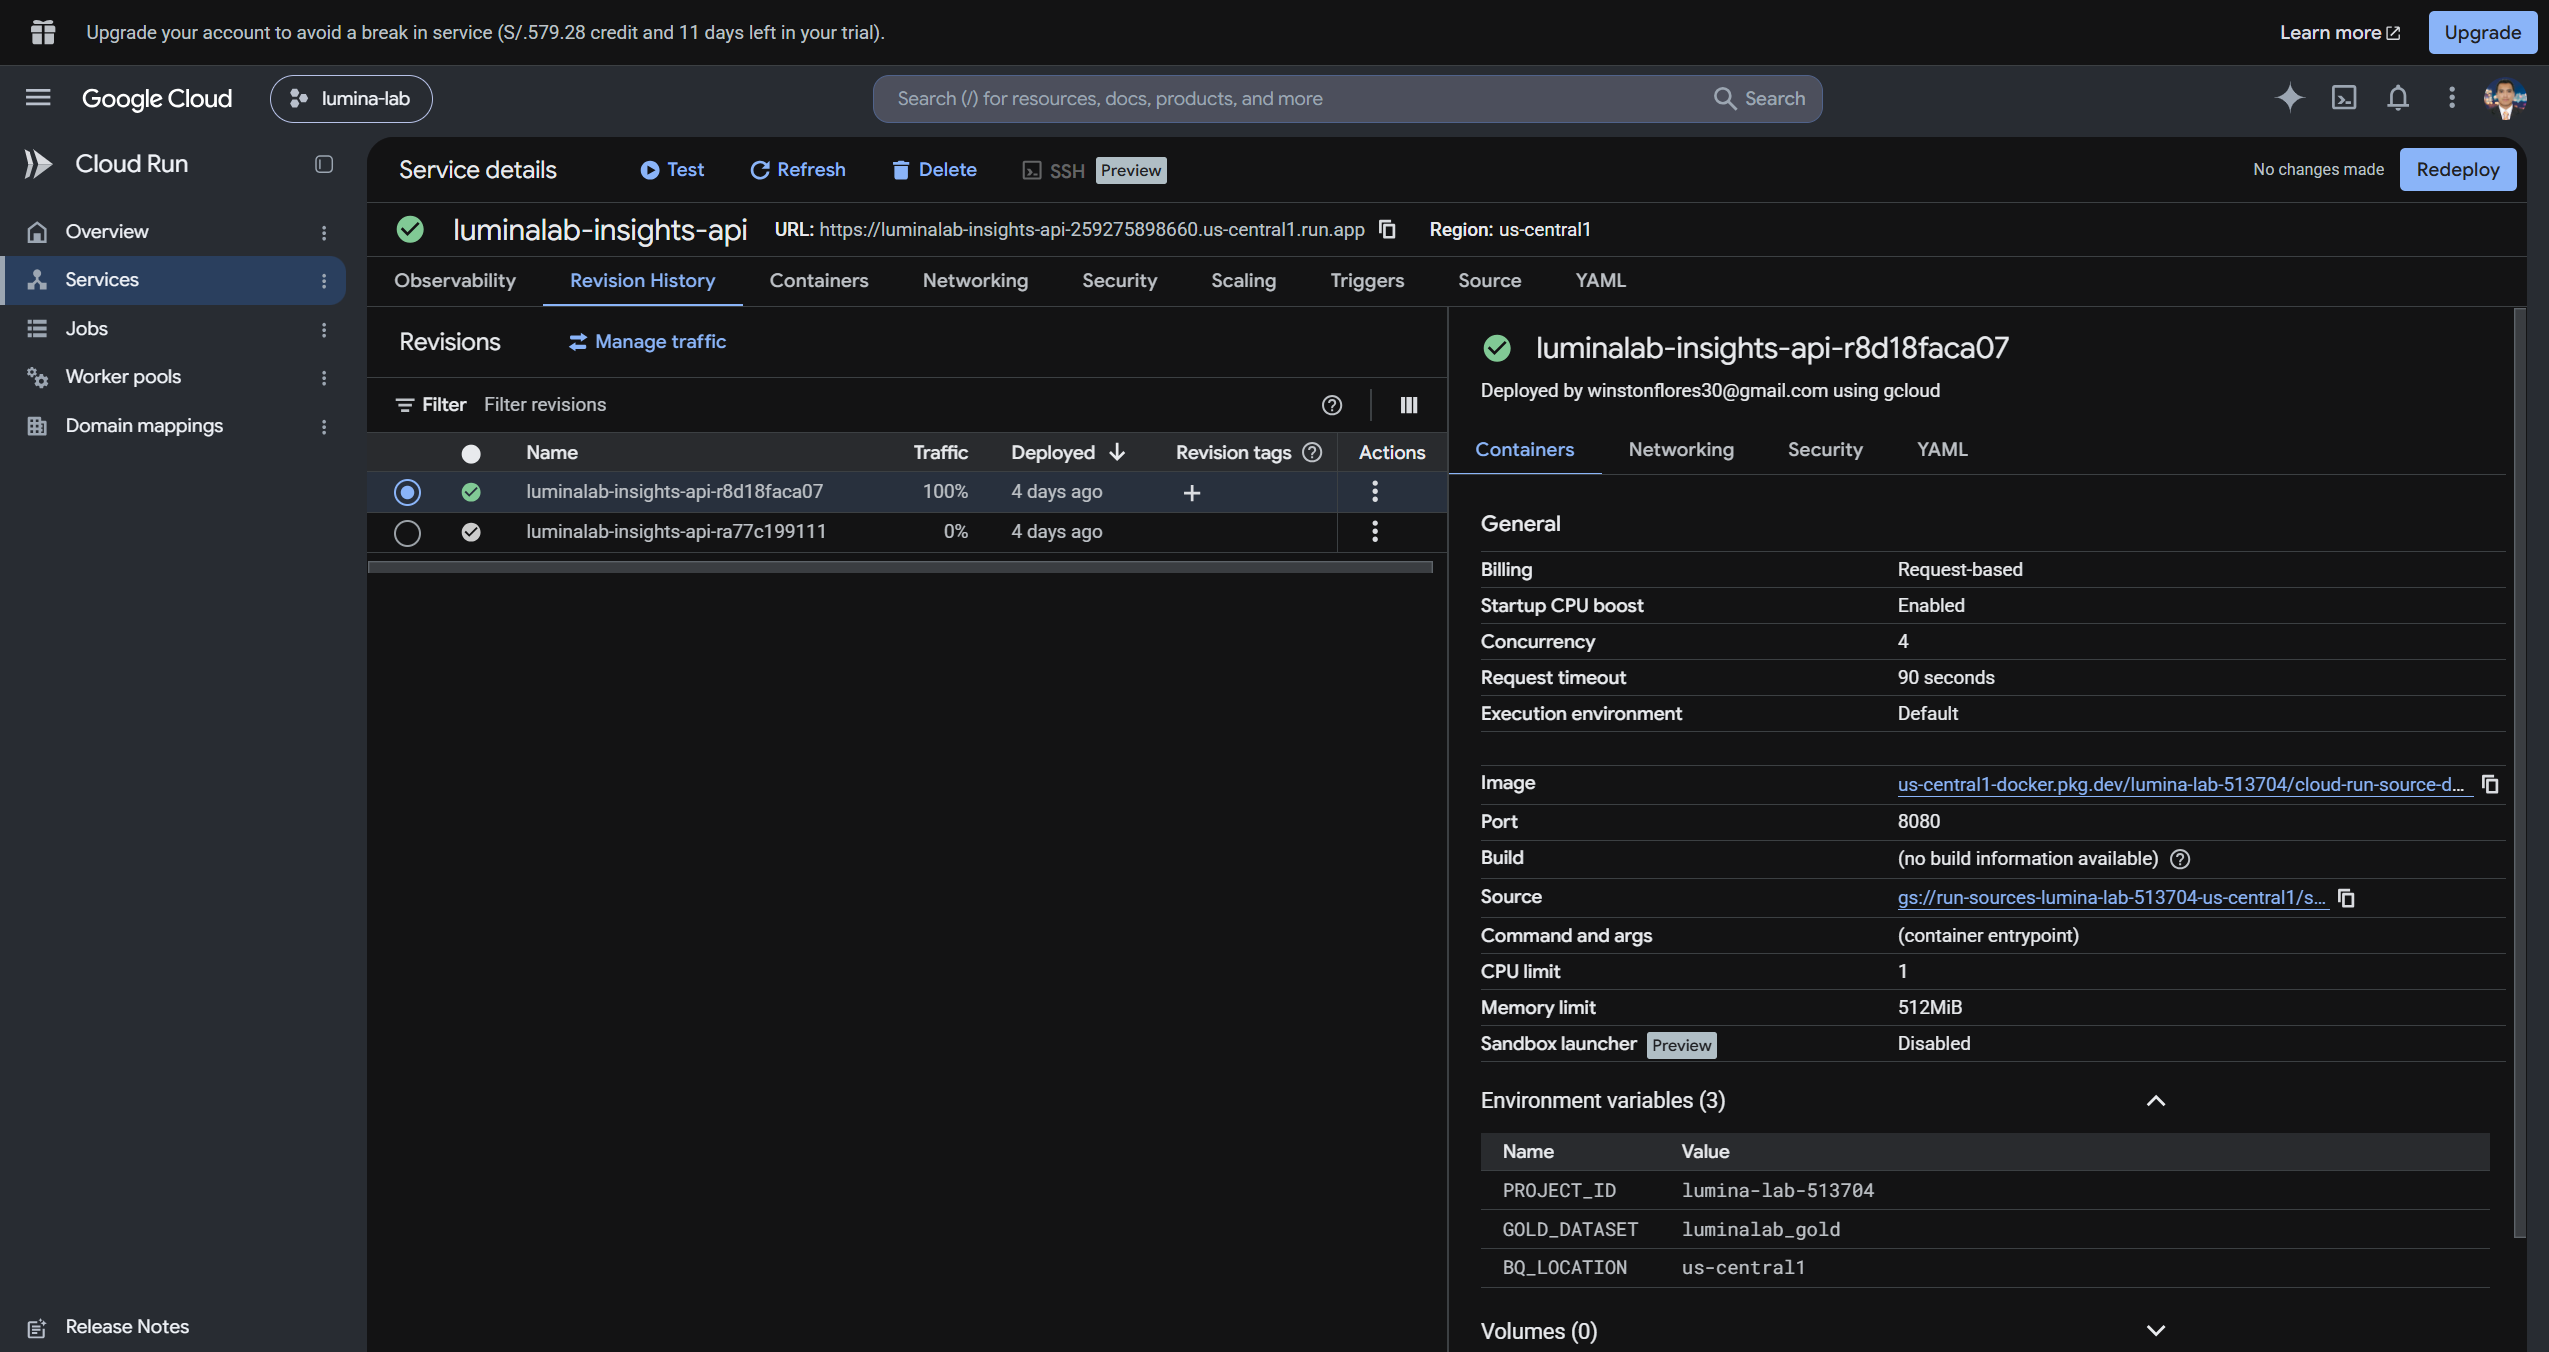
\includegraphics[width=0.96\textwidth]{../assets/evidencia/06-consumo/01-cloud-run-servicio.png}
\caption{Vista de Servicio Cloud Run privado}
\end{figure}



\begin{figure}[htbp]
\centering
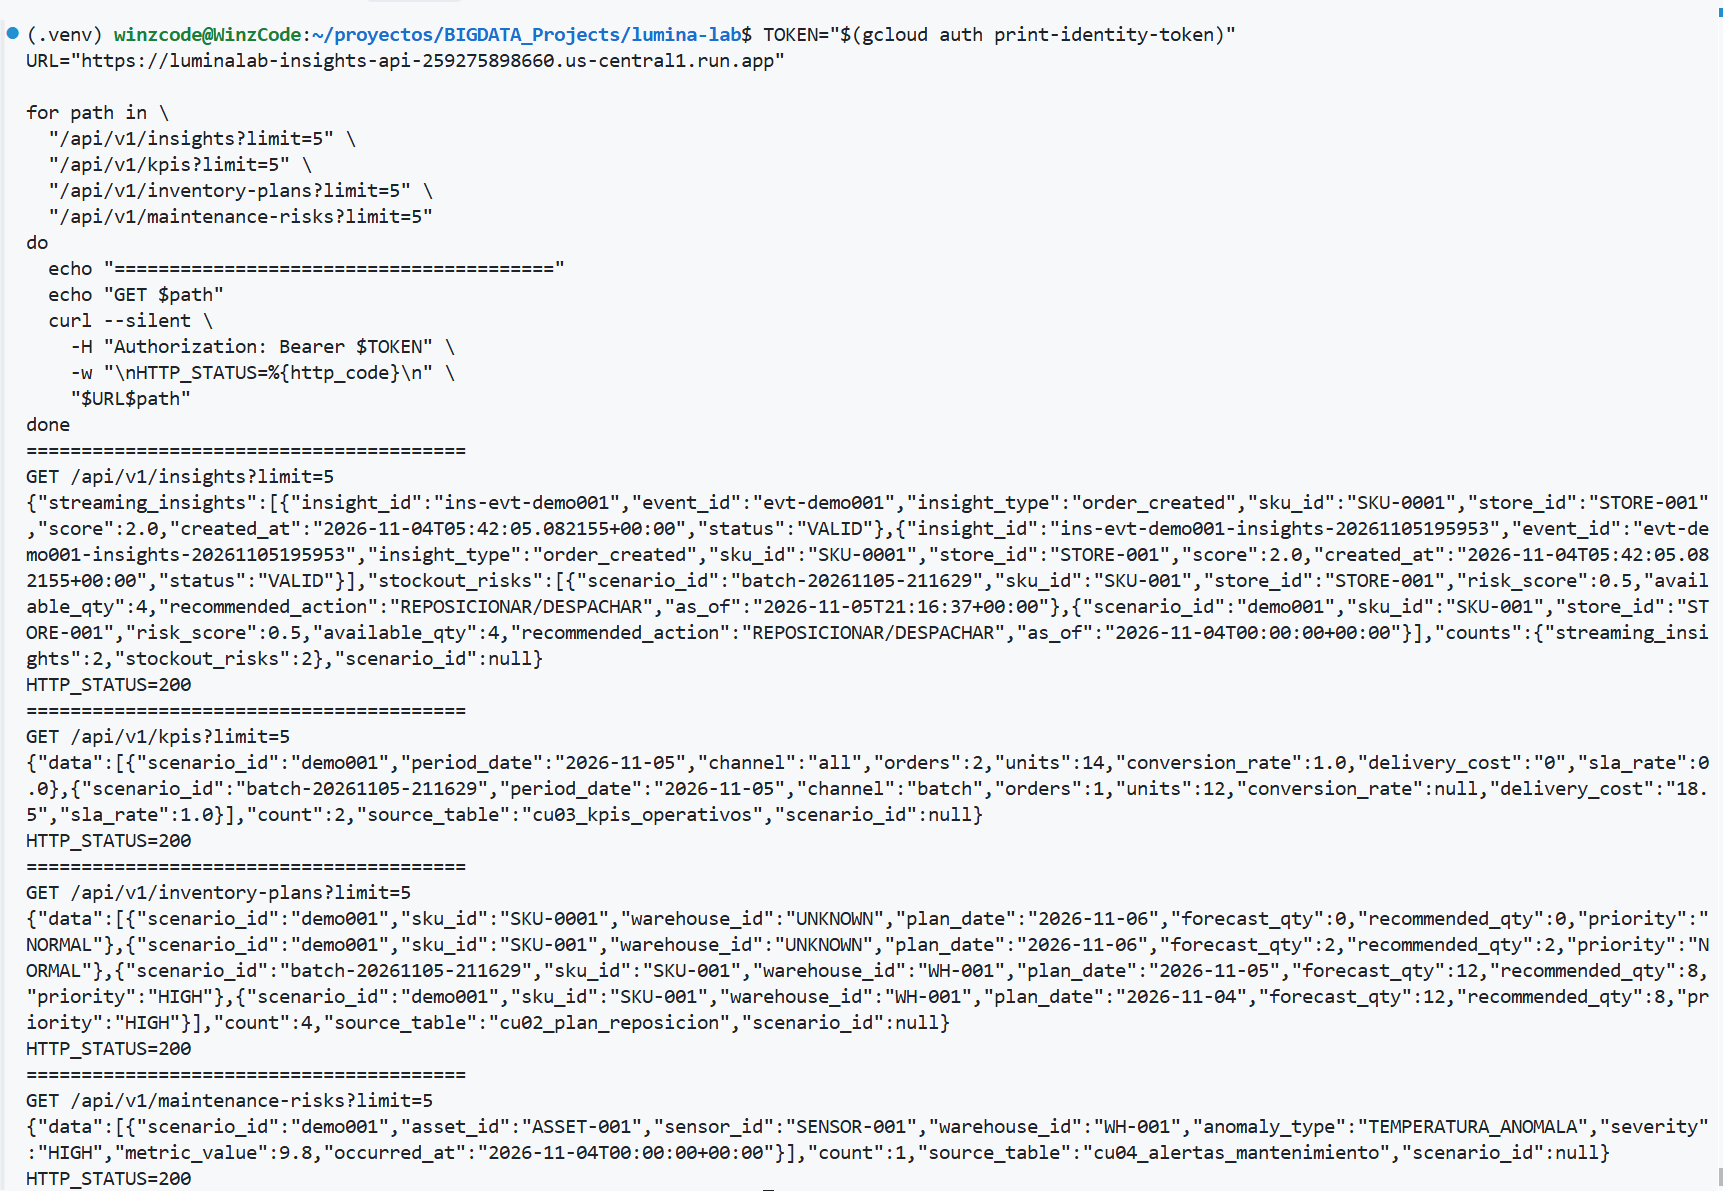
\includegraphics[width=0.96\textwidth]{../assets/evidencia/06-consumo/02-api-rutas.png}
\caption{Vista de Respuestas de negocio}
\end{figure}






\clearpage
\section{Seguridad, gobierno y observabilidad}

\begin{center}

\includegraphics[width=.4704\textwidth]{../assets/miniportadas/10-seguridad-observabilidad.png}
\end{center}

\subsection{Controles transversales}

\begingroup\small
\begin{longtable}{@{}>{\raggedright\arraybackslash}p{0.3068\textwidth}>{\raggedright\arraybackslash}p{0.3068\textwidth}>{\raggedright\arraybackslash}p{0.3068\textwidth}@{}}
\toprule
\textbf{Dominio} & \textbf{Componentes previstos/\allowbreak{}documentados} & \textbf{Evidencia que acredita} \\
\midrule
\endfirsthead
\toprule
\textbf{Dominio} & \textbf{Componentes previstos/\allowbreak{}documentados} & \textbf{Evidencia que acredita} \\
\midrule
\endhead
Gobierno & \href{https://console.cloud.google.com/dataplex/studio?referrer=search\&authuser=0\&project=prj-codenid}{Knowledge Catalog} y Data Lineage & metadatos Bronze/Silver/Gold y relaciones Gold→vista verificadas \\
Identidades & IAM por servicio & permisos mínimos worker, workflow y API \\
Cifrado & KMS y Secret Manager & claves, secreto protegido y referencias sin revelar valores \\
Protección & plantilla regional de Sensitive Data Protection & detectores EMAIL, PHONE y CARD definidos \\
Auditoría & Logging sink y BigQuery Audit Store & registro de prueba consultable \\
Observabilidad & Monitoring, alertas y SLO & métrica, política, objetivo y estado \\
\bottomrule
\end{longtable}
\endgroup

\textbf{Verificación:} el control de auditoría relaciona eventos de origen, exportación al almacén de auditoría y consulta de registros. La disponibilidad del 99 \% se establece como objetivo de servicio.\par


\begin{figure}[htbp]
\centering
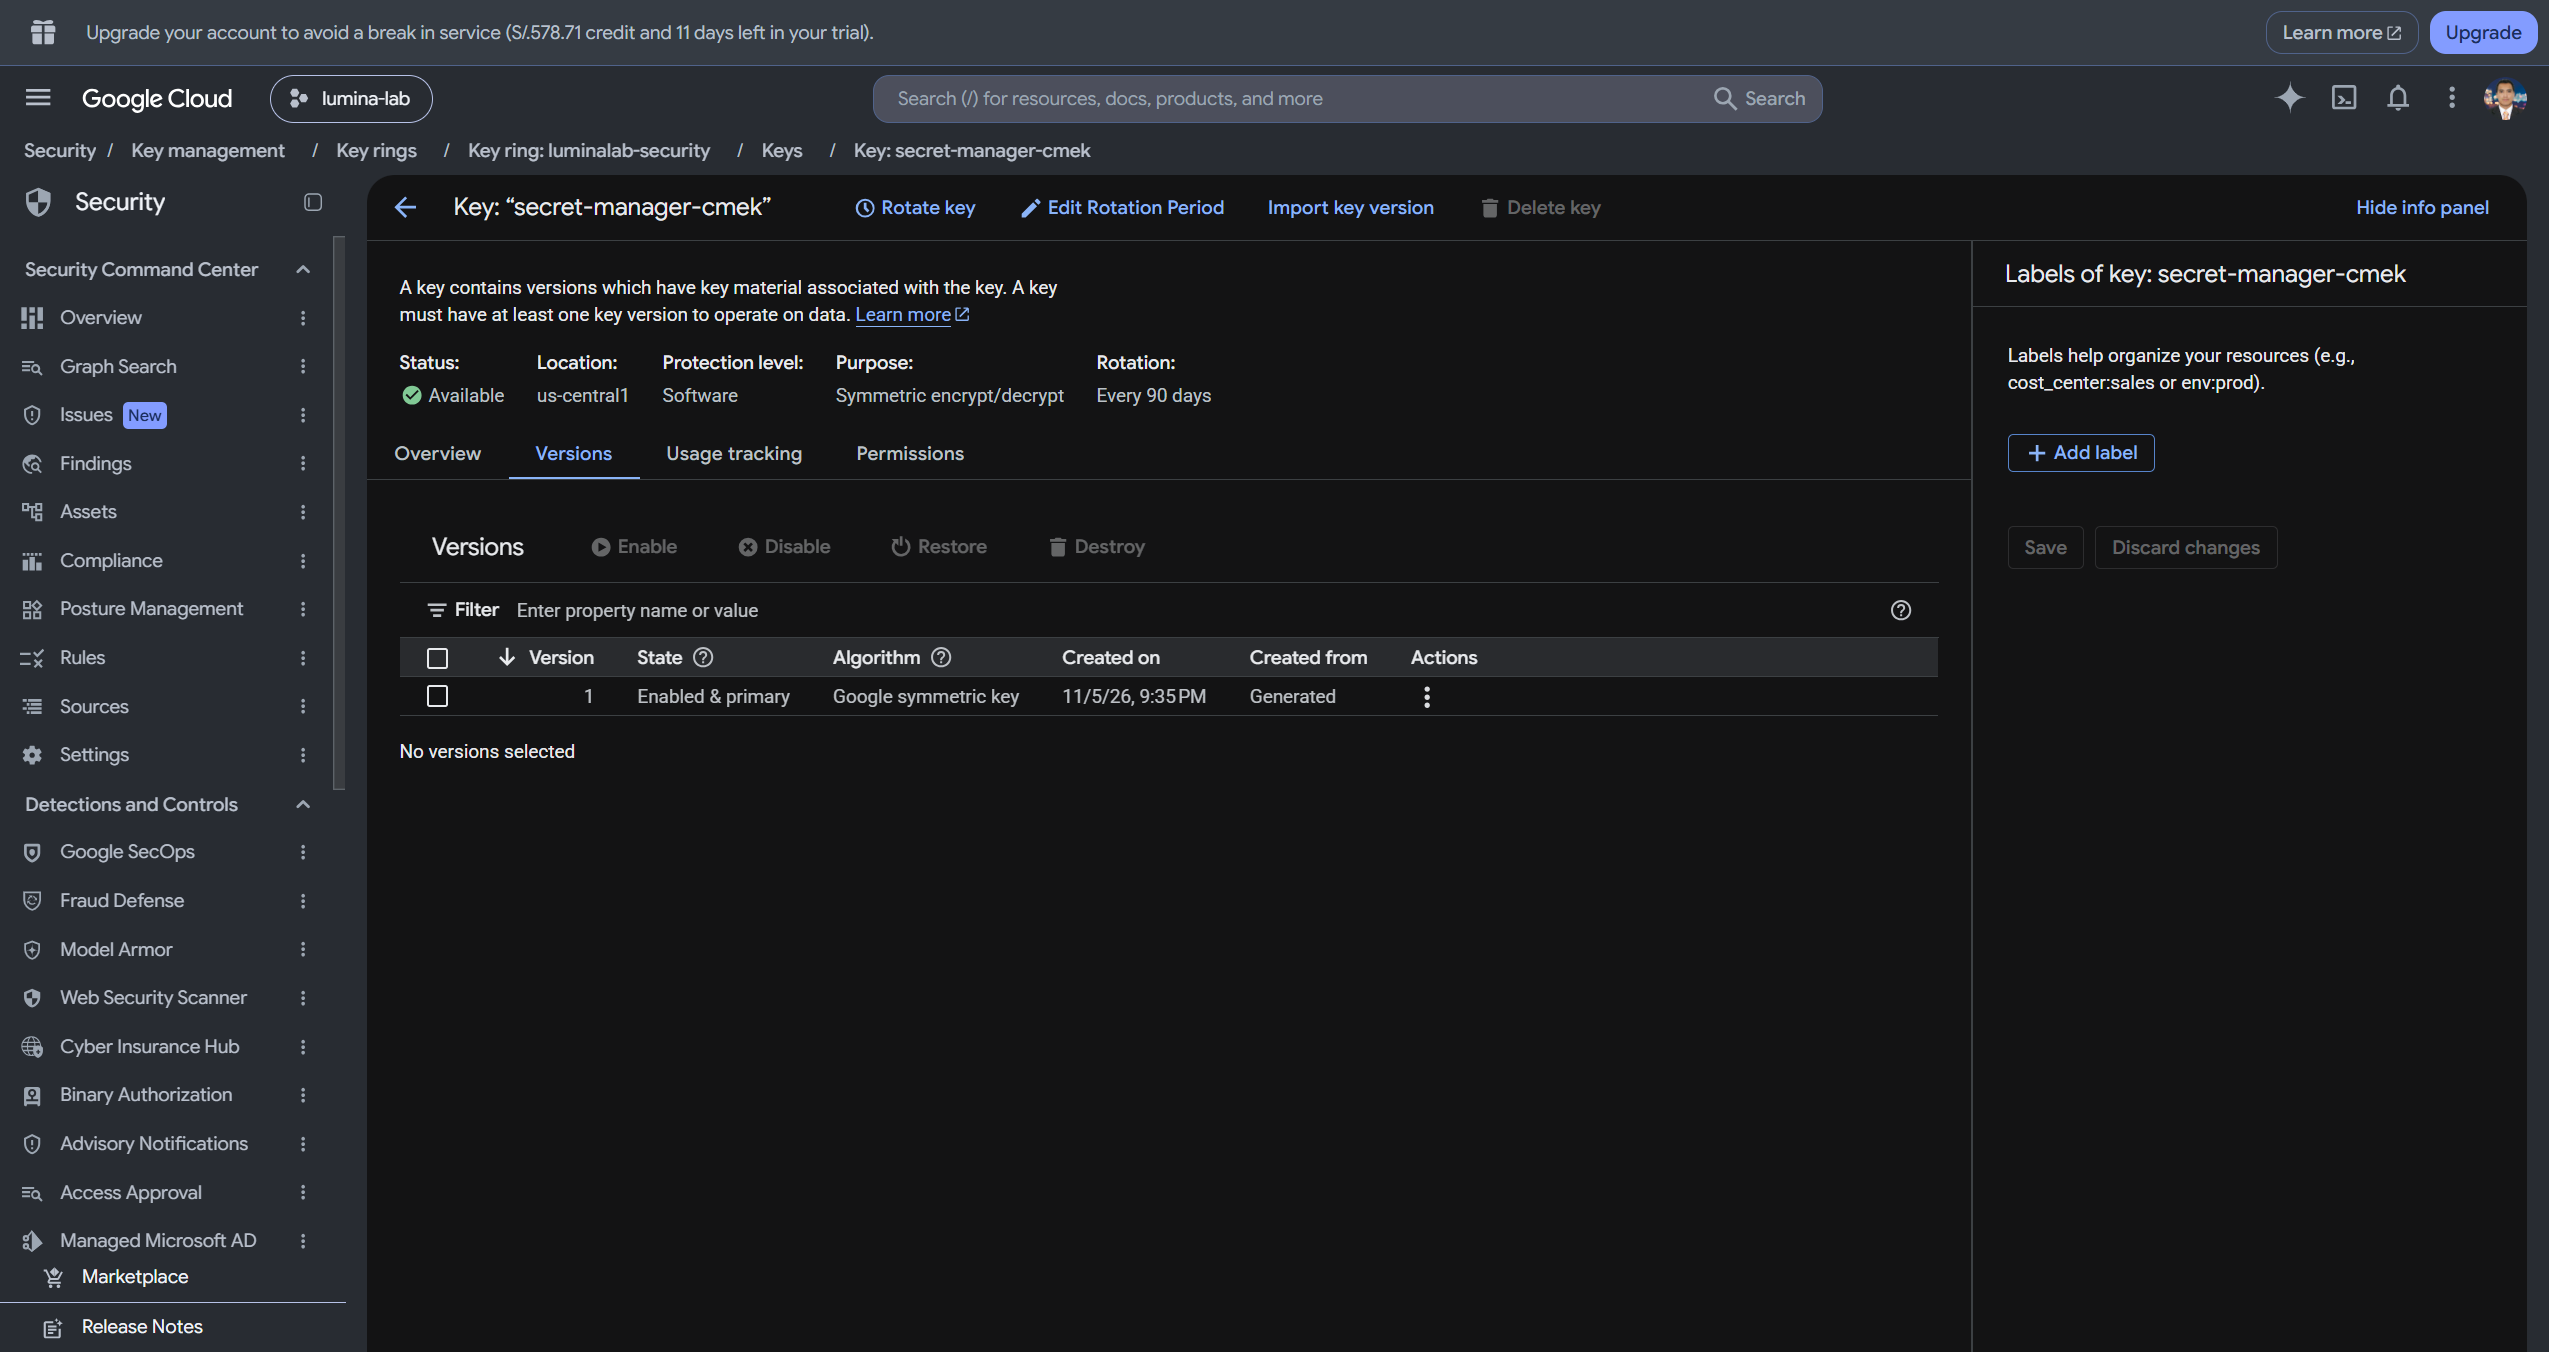
\includegraphics[width=0.96\textwidth]{../assets/evidencia/07-controles/03-seguridad-kms.png}
\caption{Configuración de la clave de cifrado en Cloud KMS}
\end{figure}

\textit{Cifrado de datos mediante Cloud KMS, sin exponer valores de secretos.}\par

\clearpage
\section{Validación end-to-end y resultados}

\begin{center}

\includegraphics[width=.4704\textwidth]{../assets/miniportadas/11-validacion-e2e.png}
\end{center}

\subsection{Resultados de las verificaciones}

\begingroup\footnotesize
\begin{longtable}{@{}>{\raggedright\arraybackslash}p{0.1468\textwidth}>{\raggedright\arraybackslash}p{0.1468\textwidth}>{\raggedright\arraybackslash}p{0.1468\textwidth}>{\raggedright\arraybackslash}p{0.1468\textwidth}>{\raggedright\arraybackslash}p{0.1468\textwidth}>{\raggedright\arraybackslash}p{0.1468\textwidth}@{}}
\toprule
\textbf{Prueba} & \textbf{Aspecto verificado} & \textbf{Evidencia} & \textbf{Resultado} & \textbf{Estado} & \textbf{Observación} \\
\midrule
\endfirsthead
\toprule
\textbf{Prueba} & \textbf{Aspecto verificado} & \textbf{Evidencia} & \textbf{Resultado} & \textbf{Estado} & \textbf{Observación} \\
\midrule
\endhead
VAL-STR-01 & Correlación por order\_\allowbreak{}id entre Bronze y Silver & Consulta Bronze y Silver & Resultado registrado & Documentado & Consulta ejecutada en BigQuery \\
VAL-STR-02 & Mismo event\_\allowbreak{}id en Insights y auditoría Gold & Consulta Insights & Resultado registrado & Documentado & Consulta ejecutada en BigQuery \\
VAL-BAT-01 & Recorrido Bronze → Silver → Gold/\allowbreak{}Mart con batch\_\allowbreak{}id & Consulta batch & Resultado registrado & Documentado & Consulta batch ejecutada \\
VAL-TRF-01 & Tipado, rechazo y deduplicación & SQL y resultado antes/\allowbreak{}después & Sin resultados observados & No validado & Sin evidencia de ejecución \\
VAL-INT-01 & Joins por claves sustentadas & SQL y resultado integrado & Sin resultados observados & No validado & Sin cardinalidades observadas \\
VAL-MOD-01 & Producto Gold con grano y medidas validados & Consulta vistas Gold & Resultado registrado & Documentado & Vistas Gold consultadas \\
VAL-API-01 & API autenticada con respuesta HTTP 200 válida & Rutas de API & Resultado registrado & Documentado & Cuatro rutas autenticadas verificadas \\
\bottomrule
\end{longtable}
\endgroup

\textbf{Cobertura de verificación:} las pruebas documentan recorridos streaming y batch, productos Gold y acceso autenticado a la API. La validación de reglas de transformación y cardinalidad de joins no cuenta con resultados registrados.\par




\clearpage
\section{Reproducibilidad y navegación del repositorio}

\begin{center}
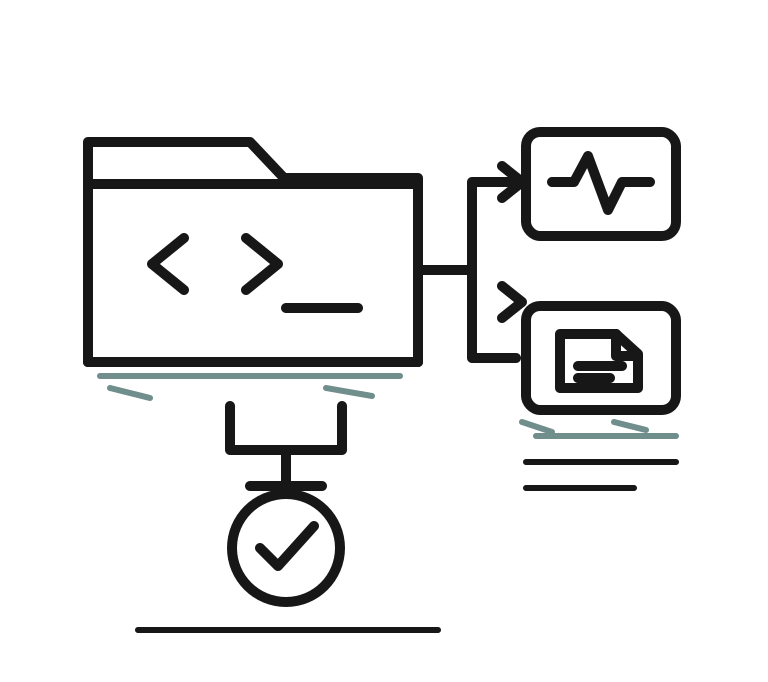
\includegraphics[width=.336\textwidth]{../assets/miniportadas/12-reproducibilidad.png}
\end{center}

Este capítulo muestra cómo está organizado el proyecto y dónde consultar cada componente y script; los enlaces llevan al detalle mantenido en el repositorio, sin duplicar el código aquí. La ejecución se ordena mediante el manifiesto y la guía operativa enlazados abajo.

\begingroup\small
\begin{longtable}{@{}>{\raggedright\arraybackslash}p{0.19\textwidth}>{\raggedright\arraybackslash}p{0.43\textwidth}>{\raggedright\arraybackslash}p{0.29\textwidth}@{}}
\toprule
\textbf{Etapa} & \textbf{Qué contiene y cómo participa} & \textbf{Referencia en el repositorio} \\
\midrule
\endfirsthead
\toprule
\textbf{Etapa} & \textbf{Qué contiene y cómo participa} & \textbf{Referencia en el repositorio} \\
\midrule
\endhead
Preparación y secuencia & Configuración local, preflight de acceso y scripts numerados. El paso 00 valida el inventario del runbook; los pasos 01--06 preparan la fundación. & \href{https://github.com/Codenid/lumina-retail-data-platform/tree/main/implementation/automatizacion/scripts}{Scripts de automatización}; \href{https://github.com/Codenid/lumina-retail-data-platform/blob/main/implementation/automatizacion/configuracion/runbook.json}{manifiesto de ejecución}. \\
Productor de datos & Perfiles de publicación streaming y batch alineados con los productores de ArchiMate. & \href{https://github.com/Codenid/lumina-retail-data-platform/tree/main/implementation/soluciones/productor-datos}{app productora}; \href{https://github.com/Codenid/lumina-retail-data-platform/blob/main/implementation/automatizacion/configuracion/contratos/productor_datos.json}{contratos}; \href{https://github.com/Codenid/lumina-retail-data-platform/blob/main/implementation/docs/arquitectura/productores.csv}{mapa de productores}. \\
Streaming & Apache Beam en Dataflow consume eventos de Pub/Sub y escribe las salidas Silver; un pipeline separado produce Insights Gold y auditoría. & \href{https://github.com/Codenid/lumina-retail-data-platform/tree/main/implementation/soluciones/procesamiento-streaming}{Código Beam}; pasos 07--13 y 43--48. \\
Batch e integración & BigQuery ejecuta cargas, curación y materialización; Workflows coordina recorridos batch. El job Spark/Dataproc se ejecuta en un clúster temporal. & \href{https://github.com/Codenid/lumina-retail-data-platform/tree/main/implementation/soluciones/orquestacion-batch}{Definición Workflows}; \href{https://github.com/Codenid/lumina-retail-data-platform/tree/main/implementation/soluciones/procesamiento-batch}{job Spark}; pasos 14--42 y 49--58. \\
Modelado y consumo & Contratos JSON y SQL describen esquemas y productos; scripts posteriores crean mart, API y vistas de reporting. & \href{https://github.com/Codenid/lumina-retail-data-platform/tree/main/implementation/automatizacion/configuracion/contratos}{Contratos y SQL}; pasos 59--69. \\
Controles y validación & Scripts de catálogo, linaje, seguridad, auditoría y observabilidad; las pruebas automatizadas verifican contratos y componentes seleccionados. & Pasos 70--83; \href{https://github.com/Codenid/lumina-retail-data-platform/tree/main/implementation/tests}{pruebas}; \href{https://github.com/Codenid/lumina-retail-data-platform/tree/main/implementation/docs/operacion}{guías operativas}. \\
\bottomrule
\end{longtable}
\endgroup

La \href{https://github.com/Codenid/lumina-retail-data-platform/blob/main/implementation/docs/operacion/ejecucion-scripts.md}{guía de ejecución} explica el orden de los grupos, dependencias, resultados esperados, reejecución y exclusiones. Los scripts 14--58 cubren casos de uso, fuentes y recorridos batch; 59--69 publican productos de consumo. La configuración sensible y el estado de cada corrida permanecen locales y fuera del control de versiones.\par

\clearpage
\section{Conclusión ejecutiva}

\begin{center}

\includegraphics[width=.4704\textwidth]{../assets/miniportadas/13-conclusion.png}
\end{center}

\subsection{Síntesis de la solución}

Lumina Retail integra ingesta streaming y batch, transformación por capas Bronze, Silver y Gold, productos analíticos para sus casos de uso y exposición mediante API privada. La solución incorpora controles de identidad, cifrado, catálogo y observabilidad para mantener los datos trazables y disponibles para el análisis operativo.\par



\clearpage
\section*{Anexo A. Inventario de interfaces y recursos}
\addcontentsline{toc}{section}{Anexo A. Inventario de interfaces y recursos}

\begingroup\small
\begin{longtable}{@{}>{\raggedright\arraybackslash}p{0.1788\textwidth}>{\raggedright\arraybackslash}p{0.1788\textwidth}>{\raggedright\arraybackslash}p{0.1788\textwidth}>{\raggedright\arraybackslash}p{0.1788\textwidth}>{\raggedright\arraybackslash}p{0.1788\textwidth}@{}}
\toprule
\textbf{Componente} & \textbf{Entrada física} & \textbf{Operación} & \textbf{Salida física} & \textbf{Referencia de implementación} \\
\midrule
\endfirsthead
\toprule
\textbf{Componente} & \textbf{Entrada física} & \textbf{Operación} & \textbf{Salida física} & \textbf{Referencia de implementación} \\
\midrule
\endhead
Generador de eventos & contrato JSON ad hoc & normaliza, asigna event\_\allowbreak{}id y publica & tópico Pub/\allowbreak{}Sub de eventos & 08\_\allowbreak{}publicar\_\allowbreak{}evento.sh \\
Pub/\allowbreak{}Sub & JSON de evento & distribuye a tres suscripciones & Dataflow pull, BigQuery raw, GCS JSONL & 05\_\allowbreak{}crear\_\allowbreak{}topicos\_\allowbreak{}y\_\allowbreak{}suscripciones.sh \\
Dataflow & suscripción pull & valida y transforma & tablas Silver & 07\_\allowbreak{}iniciar\_\allowbreak{}dataflow.sh \\
Carga batch & archivos ad hoc en Landing & parseo, carga, control de lote & BigQuery Bronze & 55\_\allowbreak{}generar\_\allowbreak{}y\_\allowbreak{}publicar\_\allowbreak{}fixtures\_\allowbreak{}batch.sh, 56\_\allowbreak{}cargar\_\allowbreak{}seis\_\allowbreak{}fuentes\_\allowbreak{}bronze.sh \\
Curación SQL & Bronze por batch\_\allowbreak{}id & SAFE\_\allowbreak{}CAST, reglas, MERGE & seis tablas Silver & 57\_\allowbreak{}curar\_\allowbreak{}seis\_\allowbreak{}fuentes\_\allowbreak{}y\_\allowbreak{}gold.sh \\
Materialización Gold & Silver validada & joins, agregaciones, cálculos & CU01-CU03, Operational Mart & 57\_\allowbreak{}curar\_\allowbreak{}seis\_\allowbreak{}fuentes\_\allowbreak{}y\_\allowbreak{}gold.sh \\
API Cloud Run & GET autenticado, filtros & consultas parametrizadas & JSON de productos Gold & soluciones/\allowbreak{}api-insights/\allowbreak{}main.py \\
Workflows & definición y parámetros de ejecución & orquestación batch & estado de ejecución y tablas destino & scripts 49-53 \\
Gobierno y observabilidad & metadatos, logs, métricas & catálogo, controles y auditoría & linaje, alertas, Audit Store & scripts 70-83 \\
\bottomrule
\end{longtable}
\endgroup

Los nombres de proyecto, prefijo, región y datasets son parametrizados. Esta tabla describe las \textbf{interfaces implementadas en código}; la comprobación del estado efectivo de GCP se conserva en las actas de operación.\par




\clearpage
\section*{Anexo B. Contratos de eventos y mensajería}
\addcontentsline{toc}{section}{Anexo B. Contratos de eventos y mensajería}

\subsection{B.1 Evento de pedido: entrada real del generador}

Fuente versionada: docs/\allowbreak{}arquitectura/\allowbreak{}contrato-evento-original.json. El script 08 actualiza event\_\allowbreak{}id, simulation\_\allowbreak{}id, trace\_\allowbreak{}id y timestamps para la ejecución; el payload del contrato es:\par

\begin{lstlisting}
{
  "schema_version": "1.1.0",
  "simulation_id": "sim-20261103-001",
  "scenario_id": "black-friday",
  "producer_id": "channel-apps",
  "event_type": "order_created",
  "event_id": "evt-000001",
  "occurred_at": "2026-11-03T10:00:00Z",
  "emitted_at": "2026-11-03T10:00:01Z",
  "trace_id": "trace-order-000001",
  "payload": {
    "order_id": "ORD-000001",
    "order_line_id": "LINE-001",
    "customer_id": "CUS-000001",
    "store_id": "STORE-001",
    "product_id": "SKU-0001",
    "quantity": 2
  }
}
\end{lstlisting}

\begingroup\small
\begin{longtable}{@{}>{\raggedright\arraybackslash}p{0.2268\textwidth}>{\raggedright\arraybackslash}p{0.2268\textwidth}>{\raggedright\arraybackslash}p{0.2268\textwidth}>{\raggedright\arraybackslash}p{0.2268\textwidth}@{}}
\toprule
\textbf{Campo} & \textbf{Tipo lógico} & \textbf{Semántica} & \textbf{Tratamiento} \\
\midrule
\endfirsthead
\toprule
\textbf{Campo} & \textbf{Tipo lógico} & \textbf{Semántica} & \textbf{Tratamiento} \\
\midrule
\endhead
schema\_\allowbreak{}version & string & versión del envelope & conservar y validar compatibilidad \\
simulation\_\allowbreak{}id / scenario\_\allowbreak{}id & string & simulación y escenario & segmentación de pruebas \\
producer\_\allowbreak{}id & string & generador ad hoc & trazabilidad \\
event\_\allowbreak{}type & string & tipo de evento, p. ej. order\_\allowbreak{}created & enrutamiento \\
event\_\allowbreak{}id & string & identificador del evento & correlación y duplicados \\
occurred\_\allowbreak{}at / emitted\_\allowbreak{}at & timestamp ISO 8601 & momento de negocio y publicación & parseo temporal \\
trace\_\allowbreak{}id & string & seguimiento distribuido & correlación \\
payload.order\_\allowbreak{}id & string & pedido & clave de negocio \\
payload.order\_\allowbreak{}line\_\allowbreak{}id & string & línea del pedido & clave compuesta Silver \\
payload.customer\_\allowbreak{}id & string & cliente simulado & atributo de negocio \\
payload.store\_\allowbreak{}id & string & tienda & dimensión \\
payload.product\_\allowbreak{}id & string & SKU del evento & Dataflow lo mapea a Silver.sku\_\allowbreak{}id \\
payload.quantity & número & unidades & entero positivo según validación de destino \\
\bottomrule
\end{longtable}
\endgroup

\textbf{Mapeo aplicado:} Dataflow convierte payload.product\_\allowbreak{}id a Silver.pedidos.sku\_\allowbreak{}id y conserva order\_\allowbreak{}id, order\_\allowbreak{}line\_\allowbreak{}id, cliente, tienda, almacén y cantidad.\par

\subsection{B.2 Topología y destinos}

\begingroup\small
\begin{longtable}{@{}>{\raggedright\arraybackslash}p{0.1788\textwidth}>{\raggedright\arraybackslash}p{0.1788\textwidth}>{\raggedright\arraybackslash}p{0.1788\textwidth}>{\raggedright\arraybackslash}p{0.1788\textwidth}>{\raggedright\arraybackslash}p{0.1788\textwidth}@{}}
\toprule
\textbf{Suscripción} & \textbf{Tipo} & \textbf{Input} & \textbf{Output} & \textbf{Consideración} \\
\midrule
\endfirsthead
\toprule
\textbf{Suscripción} & \textbf{Tipo} & \textbf{Input} & \textbf{Output} & \textbf{Consideración} \\
\midrule
\endhead
\$DF\_\allowbreak{}SUB & pull & tópico \$TOPIC & Dataflow → Silver & ack deadline 60 s; no efectuar pull manual \\
\$RAW\_\allowbreak{}BQ\_\allowbreak{}SUB & export BigQuery & tópico \$TOPIC & Bronze.eventos\_\allowbreak{}raw\_\allowbreak{}pubsub & writeMetadata=\allowbreak{}true \\
\$RAW\_\allowbreak{}SUB & export Cloud Storage & tópico \$TOPIC & bucket \$BRONZE, streaming/*.jsonl & archivos JSONL, rotación de 60 s \\
\bottomrule
\end{longtable}
\endgroup

Los tópicos de Insights y auditoría alimentan pipelines independientes. No son destinos de los seis perfiles del generador principal. La exportación a Cloud Storage conserva una copia raw adicional; no es el Landing batch.\par

\subsection{B.3 Salida raw de Pub/\allowbreak{}Sub a BigQuery}

\begingroup\small
\begin{longtable}{@{}>{\raggedright\arraybackslash}p{0.3068\textwidth}>{\raggedright\arraybackslash}p{0.3068\textwidth}>{\raggedright\arraybackslash}p{0.3068\textwidth}@{}}
\toprule
\textbf{Columna} & \textbf{Tipo BigQuery} & \textbf{Contenido} \\
\midrule
\endfirsthead
\toprule
\textbf{Columna} & \textbf{Tipo BigQuery} & \textbf{Contenido} \\
\midrule
\endhead
data & JSON & mensaje publicado \\
subscription\_\allowbreak{}name & STRING & suscripción exportadora \\
message\_\allowbreak{}id & STRING & identificador Pub/\allowbreak{}Sub \\
publish\_\allowbreak{}time & TIMESTAMP & publicación \\
attributes & JSON & atributos Pub/\allowbreak{}Sub \\
ordering\_\allowbreak{}key & STRING & clave de orden si existe \\
\bottomrule
\end{longtable}
\endgroup

\textbf{Verificación:} consultar event\_\allowbreak{}id en Bronze y order\_\allowbreak{}id/order\_\allowbreak{}line\_\allowbreak{}id en Silver. El ack de Pub/Sub no demuestra por sí solo materialización.\par




\clearpage
\section*{Anexo C. Contratos REST de consumo}
\addcontentsline{toc}{section}{Anexo C. Contratos REST de consumo}

\textbf{Implementación de referencia:} soluciones/\allowbreak{}api-insights/\allowbreak{}main.py. Todas las rutas usan \textbf{GET} y entregan application/\allowbreak{}json; charset=utf-8. El servicio Cloud Run exige invocación autenticada con IAM.\par

\subsection{C.1 Parámetros compartidos}

\begingroup\small
\begin{longtable}{@{}>{\raggedright\arraybackslash}p{0.2268\textwidth}>{\raggedright\arraybackslash}p{0.2268\textwidth}>{\raggedright\arraybackslash}p{0.2268\textwidth}>{\raggedright\arraybackslash}p{0.2268\textwidth}@{}}
\toprule
\textbf{Parámetro} & \textbf{Tipo} & \textbf{Default} & \textbf{Regla} \\
\midrule
\endfirsthead
\toprule
\textbf{Parámetro} & \textbf{Tipo} & \textbf{Default} & \textbf{Regla} \\
\midrule
\endhead
limit & integer & 25 & 1-100 inclusive \\
scenario\_\allowbreak{}id & string opcional & null & expresión \textasciicircum[][A-Za-z0-9][A-Za-z0-9.\_\allowbreak{}:-][0,127]\$ \\
\bottomrule
\end{longtable}
\endgroup

La API consulta BigQuery con parámetros enlazados, límite de facturación \textbf{52 428 800 bytes por consulta} y timeout de resultados de \textbf{60 segundos}. scenario\_\allowbreak{}id filtra tablas CU01-CU04; \textbf{no filtra} insights\_\allowbreak{}streaming.\par

\subsection{C.2 Operaciones y respuesta}

\begingroup\small
\begin{longtable}{@{}>{\raggedright\arraybackslash}p{0.3068\textwidth}>{\raggedright\arraybackslash}p{0.3068\textwidth}>{\raggedright\arraybackslash}p{0.3068\textwidth}@{}}
\toprule
\textbf{Método y ruta} & \textbf{Tablas de entrada} & \textbf{Output JSON} \\
\midrule
\endfirsthead
\toprule
\textbf{Método y ruta} & \textbf{Tablas de entrada} & \textbf{Output JSON} \\
\midrule
\endhead
GET /healthz & ninguna & [''status'':''ok''] \\
GET /api/\allowbreak{}v1/\allowbreak{}insights & insights\_\allowbreak{}streaming + cu01\_\allowbreak{}riesgo\_\allowbreak{}quiebre\_\allowbreak{}despacho & streaming\_\allowbreak{}insights[], stockout\_\allowbreak{}risks[], counts, scenario\_\allowbreak{}id \\
GET /api/\allowbreak{}v1/\allowbreak{}kpis & cu03\_\allowbreak{}kpis\_\allowbreak{}operativos & data[], count, source\_\allowbreak{}table, scenario\_\allowbreak{}id \\
GET /api/\allowbreak{}v1/\allowbreak{}inventory-plans & cu02\_\allowbreak{}plan\_\allowbreak{}reposicion & mismo envelope data[] \\
GET /api/\allowbreak{}v1/\allowbreak{}maintenance-risks & cu04\_\allowbreak{}alertas\_\allowbreak{}mantenimiento & mismo envelope data[] \\
\bottomrule
\end{longtable}
\endgroup

\textbf{Ejemplo de estructura de respuesta} (valores ilustrativos, forma derivada del código):\par

\begin{lstlisting}
{"data":[],"count":0,"source_table":"cu03_kpis_operativos","scenario_id":"demo"}
\end{lstlisting}

\textbf{Ejemplo de estructura Insights:}\par

\begin{lstlisting}
{"streaming_insights":[],"stockout_risks":[],"counts":{"streaming_insights":0,"stockout_risks":0},"scenario_id":null}
\end{lstlisting}

\subsection{C.3 Errores contractuales}

\begingroup\small
\begin{longtable}{@{}>{\raggedright\arraybackslash}p{0.3068\textwidth}>{\raggedright\arraybackslash}p{0.3068\textwidth}>{\raggedright\arraybackslash}p{0.3068\textwidth}@{}}
\toprule
\textbf{HTTP} & \textbf{Body} & \textbf{Condición} \\
\midrule
\endfirsthead
\toprule
\textbf{HTTP} & \textbf{Body} & \textbf{Condición} \\
\midrule
\endhead
400 & [''error'':''invalid\_\allowbreak{}query'',''message'':''...''] & limit o scenario\_\allowbreak{}id inválido \\
404 & [''error'':''route\_\allowbreak{}not\_\allowbreak{}found''] & ruta inexistente \\
405 & [''error'':''method\_\allowbreak{}not\_\allowbreak{}allowed''] & método distinto de GET; header Allow: GET \\
500 & [''error'':''query\_\allowbreak{}failed''] & error de consulta BigQuery \\
\bottomrule
\end{longtable}
\endgroup

Los rechazos de acceso anónimo 401/\allowbreak{}403 se gestionan en la capa Cloud Run, antes de la aplicación. El verificador 66\_\allowbreak{}verificar\_\allowbreak{}api\_\allowbreak{}retailsmart.sh exige respuestas HTTP 200 \textbf{con al menos una fila} en las cuatro rutas y valida que la API no sea accesible anónimamente.\par

\subsection{C.4 Campos de salida por producto}

- \textbf{insights\_\allowbreak{}streaming:} insight\_\allowbreak{}id, event\_\allowbreak{}id, insight\_\allowbreak{}type, sku\_\allowbreak{}id, store\_\allowbreak{}id, score, created\_\allowbreak{}at, status.\par
- \textbf{cu01\_\allowbreak{}riesgo\_\allowbreak{}quiebre\_\allowbreak{}despacho:} scenario\_\allowbreak{}id, sku\_\allowbreak{}id, store\_\allowbreak{}id, risk\_\allowbreak{}score, available\_\allowbreak{}qty, recommended\_\allowbreak{}action, as\_\allowbreak{}of.\par
- \textbf{cu02\_\allowbreak{}plan\_\allowbreak{}reposicion:} scenario\_\allowbreak{}id, sku\_\allowbreak{}id, warehouse\_\allowbreak{}id, plan\_\allowbreak{}date, forecast\_\allowbreak{}qty, recommended\_\allowbreak{}qty, priority.\par
- \textbf{cu03\_\allowbreak{}kpis\_\allowbreak{}operativos:} scenario\_\allowbreak{}id, period\_\allowbreak{}date, channel, orders, units, conversion\_\allowbreak{}rate, delivery\_\allowbreak{}cost, sla\_\allowbreak{}rate.\par
- \textbf{cu04\_\allowbreak{}alertas\_\allowbreak{}mantenimiento:} scenario\_\allowbreak{}id, asset\_\allowbreak{}id, sensor\_\allowbreak{}id, warehouse\_\allowbreak{}id, anomaly\_\allowbreak{}type, severity, metric\_\allowbreak{}value, occurred\_\allowbreak{}at.\par




\clearpage
\section*{Anexo D. Diccionario físico de datos}
\addcontentsline{toc}{section}{Anexo D. Diccionario físico de datos}

Los siguientes campos y tipos provienen de las sentencias CREATE TABLE IF NOT EXISTS de los scripts 04, 31, 44 y gold\_\allowbreak{}tables.sql. NOT NULL es la restricción declarada en el DDL. Los esquemas de tablas creadas en otros scripts se deben incorporar con el mismo método; este catálogo no sustituye una extracción del catálogo efectivo de BigQuery.\par

\subsection{<project>.<dataset>.eventos\_\allowbreak{}raw}

\begingroup\small
\begin{longtable}{@{}>{\raggedright\arraybackslash}p{0.4668\textwidth}>{\raggedright\arraybackslash}p{0.4668\textwidth}@{}}
\toprule
\textbf{Campo} & \textbf{Tipo y restricción} \\
\midrule
\endfirsthead
\toprule
\textbf{Campo} & \textbf{Tipo y restricción} \\
\midrule
\endhead
schema\_\allowbreak{}version & STRING NOT NULL \\
simulation\_\allowbreak{}id & STRING NOT NULL \\
scenario\_\allowbreak{}id & STRING NOT NULL \\
producer\_\allowbreak{}id & STRING NOT NULL \\
event\_\allowbreak{}type & STRING NOT NULL \\
event\_\allowbreak{}id & STRING NOT NULL \\
occurred\_\allowbreak{}at & TIMESTAMP NOT NULL \\
emitted\_\allowbreak{}at & TIMESTAMP NOT NULL \\
ingested\_\allowbreak{}at & TIMESTAMP \\
trace\_\allowbreak{}id & STRING NOT NULL \\
source\_\allowbreak{}system & STRING \\
payload\_\allowbreak{}json & JSON \\
is\_\allowbreak{}valid & BOOL \\
\bottomrule
\end{longtable}
\endgroup

\subsection{<project>.<dataset>.eventos\_\allowbreak{}raw\_\allowbreak{}pubsub}

\begingroup\small
\begin{longtable}{@{}>{\raggedright\arraybackslash}p{0.4668\textwidth}>{\raggedright\arraybackslash}p{0.4668\textwidth}@{}}
\toprule
\textbf{Campo} & \textbf{Tipo y restricción} \\
\midrule
\endfirsthead
\toprule
\textbf{Campo} & \textbf{Tipo y restricción} \\
\midrule
\endhead
data & JSON \\
subscription\_\allowbreak{}name & STRING \\
message\_\allowbreak{}id & STRING \\
publish\_\allowbreak{}time & TIMESTAMP \\
attributes & JSON \\
ordering\_\allowbreak{}key & STRING \\
\bottomrule
\end{longtable}
\endgroup

\subsection{<project>.<dataset>.\$[table]\_\allowbreak{}raw}

\begingroup\small
\begin{longtable}{@{}>{\raggedright\arraybackslash}p{0.4668\textwidth}>{\raggedright\arraybackslash}p{0.4668\textwidth}@{}}
\toprule
\textbf{Campo} & \textbf{Tipo y restricción} \\
\midrule
\endfirsthead
\toprule
\textbf{Campo} & \textbf{Tipo y restricción} \\
\midrule
\endhead
batch\_\allowbreak{}id & STRING NOT NULL \\
file\_\allowbreak{}id & STRING NOT NULL \\
source\_\allowbreak{}file\_\allowbreak{}uri & STRING NOT NULL \\
source\_\allowbreak{}system & STRING NOT NULL \\
source\_\allowbreak{}row\_\allowbreak{}number & INT64 NOT NULL \\
ingested\_\allowbreak{}at & TIMESTAMP NOT NULL \\
effective\_\allowbreak{}at & TIMESTAMP \\
record\_\allowbreak{}hash & STRING NOT NULL \\
payload\_\allowbreak{}json & JSON NOT NULL \\
is\_\allowbreak{}valid & BOOL NOT NULL \\
error\_\allowbreak{}reason & STRING \\
\bottomrule
\end{longtable}
\endgroup

\subsection{<project>.<dataset>.pedidos}

\begingroup\small
\begin{longtable}{@{}>{\raggedright\arraybackslash}p{0.4668\textwidth}>{\raggedright\arraybackslash}p{0.4668\textwidth}@{}}
\toprule
\textbf{Campo} & \textbf{Tipo y restricción} \\
\midrule
\endfirsthead
\toprule
\textbf{Campo} & \textbf{Tipo y restricción} \\
\midrule
\endhead
order\_\allowbreak{}id & STRING NOT NULL \\
order\_\allowbreak{}line\_\allowbreak{}id & STRING \\
customer\_\allowbreak{}id & STRING \\
store\_\allowbreak{}id & STRING \\
warehouse\_\allowbreak{}id & STRING \\
sku\_\allowbreak{}id & STRING NOT NULL \\
quantity & INT64 NOT NULL \\
occurred\_\allowbreak{}at & TIMESTAMP NOT NULL \\
quality\_\allowbreak{}status & STRING NOT NULL \\
\bottomrule
\end{longtable}
\endgroup

\subsection{<project>.<dataset>.inventario}

\begingroup\small
\begin{longtable}{@{}>{\raggedright\arraybackslash}p{0.4668\textwidth}>{\raggedright\arraybackslash}p{0.4668\textwidth}@{}}
\toprule
\textbf{Campo} & \textbf{Tipo y restricción} \\
\midrule
\endfirsthead
\toprule
\textbf{Campo} & \textbf{Tipo y restricción} \\
\midrule
\endhead
snapshot\_\allowbreak{}id & STRING NOT NULL \\
warehouse\_\allowbreak{}id & STRING NOT NULL \\
store\_\allowbreak{}id & STRING \\
sku\_\allowbreak{}id & STRING NOT NULL \\
on\_\allowbreak{}hand\_\allowbreak{}qty & INT64 NOT NULL \\
reserved\_\allowbreak{}qty & INT64 NOT NULL \\
effective\_\allowbreak{}at & TIMESTAMP NOT NULL \\
quality\_\allowbreak{}status & STRING NOT NULL \\
\bottomrule
\end{longtable}
\endgroup

\subsection{<project>.<dataset>.entregas}

\begingroup\small
\begin{longtable}{@{}>{\raggedright\arraybackslash}p{0.4668\textwidth}>{\raggedright\arraybackslash}p{0.4668\textwidth}@{}}
\toprule
\textbf{Campo} & \textbf{Tipo y restricción} \\
\midrule
\endfirsthead
\toprule
\textbf{Campo} & \textbf{Tipo y restricción} \\
\midrule
\endhead
delivery\_\allowbreak{}id & STRING NOT NULL \\
order\_\allowbreak{}id & STRING NOT NULL \\
store\_\allowbreak{}id & STRING \\
region\_\allowbreak{}id & STRING \\
promised\_\allowbreak{}at & TIMESTAMP \\
delivered\_\allowbreak{}at & TIMESTAMP \\
delivery\_\allowbreak{}cost & NUMERIC \\
quality\_\allowbreak{}status & STRING NOT NULL \\
\bottomrule
\end{longtable}
\endgroup

\subsection{<project>.<dataset>.telemetria\_\allowbreak{}activos}

\begingroup\small
\begin{longtable}{@{}>{\raggedright\arraybackslash}p{0.4668\textwidth}>{\raggedright\arraybackslash}p{0.4668\textwidth}@{}}
\toprule
\textbf{Campo} & \textbf{Tipo y restricción} \\
\midrule
\endfirsthead
\toprule
\textbf{Campo} & \textbf{Tipo y restricción} \\
\midrule
\endhead
asset\_\allowbreak{}id & STRING NOT NULL \\
sensor\_\allowbreak{}id & STRING NOT NULL \\
warehouse\_\allowbreak{}id & STRING \\
store\_\allowbreak{}id & STRING \\
metric\_\allowbreak{}name & STRING NOT NULL \\
metric\_\allowbreak{}value & FLOAT64 NOT NULL \\
unit & STRING NOT NULL \\
occurred\_\allowbreak{}at & TIMESTAMP NOT NULL \\
quality\_\allowbreak{}status & STRING NOT NULL \\
\bottomrule
\end{longtable}
\endgroup

\subsection{<project>.<dataset>.\$table}

\begingroup\small
\begin{longtable}{@{}>{\raggedright\arraybackslash}p{0.4668\textwidth}>{\raggedright\arraybackslash}p{0.4668\textwidth}@{}}
\toprule
\textbf{Campo} & \textbf{Tipo y restricción} \\
\midrule
\endfirsthead
\toprule
\textbf{Campo} & \textbf{Tipo y restricción} \\
\midrule
\endhead
batch\_\allowbreak{}id & STRING NOT NULL \\
file\_\allowbreak{}id & STRING NOT NULL \\
source\_\allowbreak{}file\_\allowbreak{}uri & STRING NOT NULL \\
source\_\allowbreak{}system & STRING NOT NULL \\
source\_\allowbreak{}row\_\allowbreak{}number & INT64 NOT NULL \\
ingested\_\allowbreak{}at & TIMESTAMP NOT NULL \\
effective\_\allowbreak{}at & TIMESTAMP \\
record\_\allowbreak{}hash & STRING NOT NULL \\
payload\_\allowbreak{}json & JSON NOT NULL \\
is\_\allowbreak{}valid & BOOL NOT NULL \\
error\_\allowbreak{}reason & STRING \\
\bottomrule
\end{longtable}
\endgroup

\subsection{<project>.<dataset>.benchmark\_\allowbreak{}competidores}

\begingroup\small
\begin{longtable}{@{}>{\raggedright\arraybackslash}p{0.4668\textwidth}>{\raggedright\arraybackslash}p{0.4668\textwidth}@{}}
\toprule
\textbf{Campo} & \textbf{Tipo y restricción} \\
\midrule
\endfirsthead
\toprule
\textbf{Campo} & \textbf{Tipo y restricción} \\
\midrule
\endhead
benchmark\_\allowbreak{}id & STRING NOT NULL \\
competitor\_\allowbreak{}id & STRING NOT NULL \\
sku\_\allowbreak{}id & STRING NOT NULL \\
store\_\allowbreak{}id & STRING \\
observed\_\allowbreak{}at & TIMESTAMP NOT NULL \\
competitor\_\allowbreak{}price & NUMERIC NOT NULL \\
availability & STRING \\
quality\_\allowbreak{}status & STRING NOT NULL \\
\bottomrule
\end{longtable}
\endgroup

\subsection{<project>.<dataset>.eventos\_\allowbreak{}locales}

\begingroup\small
\begin{longtable}{@{}>{\raggedright\arraybackslash}p{0.4668\textwidth}>{\raggedright\arraybackslash}p{0.4668\textwidth}@{}}
\toprule
\textbf{Campo} & \textbf{Tipo y restricción} \\
\midrule
\endfirsthead
\toprule
\textbf{Campo} & \textbf{Tipo y restricción} \\
\midrule
\endhead
local\_\allowbreak{}event\_\allowbreak{}id & STRING NOT NULL \\
store\_\allowbreak{}id & STRING NOT NULL \\
event\_\allowbreak{}type & STRING NOT NULL \\
start\_\allowbreak{}at & TIMESTAMP NOT NULL \\
end\_\allowbreak{}at & TIMESTAMP \\
impact\_\allowbreak{}score & FLOAT64 NOT NULL \\
quality\_\allowbreak{}status & STRING NOT NULL \\
\bottomrule
\end{longtable}
\endgroup

\subsection{<project>.<dataset>.redes\_\allowbreak{}sociales}

\begingroup\small
\begin{longtable}{@{}>{\raggedright\arraybackslash}p{0.4668\textwidth}>{\raggedright\arraybackslash}p{0.4668\textwidth}@{}}
\toprule
\textbf{Campo} & \textbf{Tipo y restricción} \\
\midrule
\endfirsthead
\toprule
\textbf{Campo} & \textbf{Tipo y restricción} \\
\midrule
\endhead
post\_\allowbreak{}id & STRING NOT NULL \\
platform & STRING NOT NULL \\
published\_\allowbreak{}at & TIMESTAMP NOT NULL \\
sku\_\allowbreak{}id & STRING NOT NULL \\
sentiment\_\allowbreak{}score & FLOAT64 NOT NULL \\
engagement\_\allowbreak{}count & INT64 NOT NULL \\
text\_\allowbreak{}hash & STRING NOT NULL \\
quality\_\allowbreak{}status & STRING NOT NULL \\
\bottomrule
\end{longtable}
\endgroup

\subsection{<project>.<dataset>.insights\_\allowbreak{}streaming}

\begingroup\small
\begin{longtable}{@{}>{\raggedright\arraybackslash}p{0.4668\textwidth}>{\raggedright\arraybackslash}p{0.4668\textwidth}@{}}
\toprule
\textbf{Campo} & \textbf{Tipo y restricción} \\
\midrule
\endfirsthead
\toprule
\textbf{Campo} & \textbf{Tipo y restricción} \\
\midrule
\endhead
insight\_\allowbreak{}id & STRING NOT NULL \\
event\_\allowbreak{}id & STRING NOT NULL \\
insight\_\allowbreak{}type & STRING NOT NULL \\
sku\_\allowbreak{}id & STRING \\
store\_\allowbreak{}id & STRING \\
score & FLOAT64 \\
created\_\allowbreak{}at & TIMESTAMP NOT NULL \\
status & STRING NOT NULL \\
\bottomrule
\end{longtable}
\endgroup

\subsection{<project>.<dataset>.procesamiento\_\allowbreak{}auditoria}

\begingroup\small
\begin{longtable}{@{}>{\raggedright\arraybackslash}p{0.4668\textwidth}>{\raggedright\arraybackslash}p{0.4668\textwidth}@{}}
\toprule
\textbf{Campo} & \textbf{Tipo y restricción} \\
\midrule
\endfirsthead
\toprule
\textbf{Campo} & \textbf{Tipo y restricción} \\
\midrule
\endhead
audit\_\allowbreak{}id & STRING NOT NULL \\
event\_\allowbreak{}id & STRING NOT NULL \\
component & STRING NOT NULL \\
status & STRING NOT NULL \\
observed\_\allowbreak{}at & TIMESTAMP NOT NULL \\
detail & STRING \\
\bottomrule
\end{longtable}
\endgroup

\subsection{<project>.<dataset>.cu01\_\allowbreak{}riesgo\_\allowbreak{}quiebre\_\allowbreak{}despacho}

\begingroup\small
\begin{longtable}{@{}>{\raggedright\arraybackslash}p{0.4668\textwidth}>{\raggedright\arraybackslash}p{0.4668\textwidth}@{}}
\toprule
\textbf{Campo} & \textbf{Tipo y restricción} \\
\midrule
\endfirsthead
\toprule
\textbf{Campo} & \textbf{Tipo y restricción} \\
\midrule
\endhead
scenario\_\allowbreak{}id & STRING \\
sku\_\allowbreak{}id & STRING \\
store\_\allowbreak{}id & STRING \\
risk\_\allowbreak{}score & FLOAT64 \\
available\_\allowbreak{}qty & INT64 \\
recommended\_\allowbreak{}action & STRING \\
as\_\allowbreak{}of & TIMESTAMP \\
\bottomrule
\end{longtable}
\endgroup

\subsection{<project>.<dataset>.cu02\_\allowbreak{}plan\_\allowbreak{}reposicion}

\begingroup\small
\begin{longtable}{@{}>{\raggedright\arraybackslash}p{0.4668\textwidth}>{\raggedright\arraybackslash}p{0.4668\textwidth}@{}}
\toprule
\textbf{Campo} & \textbf{Tipo y restricción} \\
\midrule
\endfirsthead
\toprule
\textbf{Campo} & \textbf{Tipo y restricción} \\
\midrule
\endhead
scenario\_\allowbreak{}id & STRING \\
sku\_\allowbreak{}id & STRING \\
warehouse\_\allowbreak{}id & STRING \\
plan\_\allowbreak{}date & DATE \\
forecast\_\allowbreak{}qty & INT64 \\
recommended\_\allowbreak{}qty & INT64 \\
priority & STRING \\
\bottomrule
\end{longtable}
\endgroup

\subsection{<project>.<dataset>.cu03\_\allowbreak{}kpis\_\allowbreak{}operativos}

\begingroup\small
\begin{longtable}{@{}>{\raggedright\arraybackslash}p{0.4668\textwidth}>{\raggedright\arraybackslash}p{0.4668\textwidth}@{}}
\toprule
\textbf{Campo} & \textbf{Tipo y restricción} \\
\midrule
\endfirsthead
\toprule
\textbf{Campo} & \textbf{Tipo y restricción} \\
\midrule
\endhead
scenario\_\allowbreak{}id & STRING \\
period\_\allowbreak{}date & DATE \\
channel & STRING \\
orders & INT64 \\
units & INT64 \\
conversion\_\allowbreak{}rate & FLOAT64 \\
delivery\_\allowbreak{}cost & NUMERIC \\
sla\_\allowbreak{}rate & FLOAT64 \\
\bottomrule
\end{longtable}
\endgroup

\subsection{<project>.<dataset>.cu04\_\allowbreak{}alertas\_\allowbreak{}mantenimiento}

\begingroup\small
\begin{longtable}{@{}>{\raggedright\arraybackslash}p{0.4668\textwidth}>{\raggedright\arraybackslash}p{0.4668\textwidth}@{}}
\toprule
\textbf{Campo} & \textbf{Tipo y restricción} \\
\midrule
\endfirsthead
\toprule
\textbf{Campo} & \textbf{Tipo y restricción} \\
\midrule
\endhead
scenario\_\allowbreak{}id & STRING \\
asset\_\allowbreak{}id & STRING \\
sensor\_\allowbreak{}id & STRING \\
warehouse\_\allowbreak{}id & STRING \\
anomaly\_\allowbreak{}type & STRING \\
severity & STRING \\
metric\_\allowbreak{}value & FLOAT64 \\
occurred\_\allowbreak{}at & TIMESTAMP \\
\bottomrule
\end{longtable}
\endgroup


\textbf{Controles de integridad:} BigQuery no garantiza unicidad mediante estas definiciones; la idempotencia se implementa en MERGE y filtros de ejecución. La nulabilidad y los esquemas reales deben contrastarse con INFORMATION\_\allowbreak{}SCHEMA.COLUMNS cuando haya recursos desplegados.\par




\clearpage
\section*{Anexo E. Contratos de archivos y procesamiento batch}
\addcontentsline{toc}{section}{Anexo E. Contratos de archivos y procesamiento batch}

Fuente versionada: automatizacion/\allowbreak{}configuracion/\allowbreak{}contratos/\allowbreak{}batch\_\allowbreak{}sources.json (v1.1). \textbf{Todos los dominios corresponden a fixtures propios ad hoc}, aunque sus nombres de productor simulen sistemas empresariales.\par

\begingroup\small
\begin{longtable}{@{}>{\raggedright\arraybackslash}p{0.1788\textwidth}>{\raggedright\arraybackslash}p{0.1788\textwidth}>{\raggedright\arraybackslash}p{0.1788\textwidth}>{\raggedright\arraybackslash}p{0.1788\textwidth}>{\raggedright\arraybackslash}p{0.1788\textwidth}@{}}
\toprule
\textbf{Dominio} & \textbf{Productor simulado} & \textbf{Entrada (payload JSON)} & \textbf{Clave} & \textbf{Destino Bronze → Silver} \\
\midrule
\endfirsthead
\toprule
\textbf{Dominio} & \textbf{Productor simulado} & \textbf{Entrada (payload JSON)} & \textbf{Clave} & \textbf{Destino Bronze → Silver} \\
\midrule
\endhead
pedidos & Sistema de Pedidos & order\_\allowbreak{}id, order\_\allowbreak{}line\_\allowbreak{}id, customer\_\allowbreak{}id, store\_\allowbreak{}id, warehouse\_\allowbreak{}id, sku\_\allowbreak{}id, quantity, occurred\_\allowbreak{}at & order\_\allowbreak{}id + order\_\allowbreak{}line\_\allowbreak{}id & pedidos\_\allowbreak{}raw → pedidos \\
inventario & ERP / Sistema de Inventario & snapshot\_\allowbreak{}id, warehouse\_\allowbreak{}id, store\_\allowbreak{}id, sku\_\allowbreak{}id, on\_\allowbreak{}hand\_\allowbreak{}qty, reserved\_\allowbreak{}qty, effective\_\allowbreak{}at & snapshot\_\allowbreak{}id & inventario\_\allowbreak{}raw → inventario \\
entregas & Aplicación de Almacenes & delivery\_\allowbreak{}id, order\_\allowbreak{}id, store\_\allowbreak{}id, region\_\allowbreak{}id, promised\_\allowbreak{}at, delivered\_\allowbreak{}at, delivery\_\allowbreak{}cost & delivery\_\allowbreak{}id & entregas\_\allowbreak{}raw → entregas \\
benchmark\_\allowbreak{}competidores & Benchmark Competidores & benchmark\_\allowbreak{}id, competitor\_\allowbreak{}id, sku\_\allowbreak{}id, store\_\allowbreak{}id, observed\_\allowbreak{}at, competitor\_\allowbreak{}price, availability, source\_\allowbreak{}uri & benchmark\_\allowbreak{}id & benchmark\_\allowbreak{}competidores\_\allowbreak{}raw → benchmark\_\allowbreak{}competidores \\
eventos\_\allowbreak{}locales & Eventos Locales & local\_\allowbreak{}event\_\allowbreak{}id, store\_\allowbreak{}id, event\_\allowbreak{}type, start\_\allowbreak{}at, end\_\allowbreak{}at, impact\_\allowbreak{}score, source\_\allowbreak{}uri & local\_\allowbreak{}event\_\allowbreak{}id & eventos\_\allowbreak{}locales\_\allowbreak{}raw → eventos\_\allowbreak{}locales \\
redes\_\allowbreak{}sociales & Redes Sociales & post\_\allowbreak{}id, platform, published\_\allowbreak{}at, sku\_\allowbreak{}id, sentiment\_\allowbreak{}score, engagement\_\allowbreak{}count, text\_\allowbreak{}hash, source\_\allowbreak{}uri & post\_\allowbreak{}id & redes\_\allowbreak{}sociales\_\allowbreak{}raw → redes\_\allowbreak{}sociales \\
\bottomrule
\end{longtable}
\endgroup

\textbf{Proyección de campos:} Bronze conserva el payload original. Silver publica las columnas tipadas definidas por su esquema; source\_\allowbreak{}uri de competidores, eventos locales y redes sociales permanece en Bronze y no se proyecta a Silver. La procedencia del archivo se conserva además en source\_\allowbreak{}file\_\allowbreak{}uri del envelope.\par

\subsection{E.1 Envelope físico Bronze para lotes}

Las tablas *\_\allowbreak{}raw usan el mismo esquema:\par

\begingroup\small
\begin{longtable}{@{}>{\raggedright\arraybackslash}p{0.3068\textwidth}>{\raggedright\arraybackslash}p{0.3068\textwidth}>{\raggedright\arraybackslash}p{0.3068\textwidth}@{}}
\toprule
\textbf{Campo} & \textbf{Tipo} & \textbf{Significado} \\
\midrule
\endfirsthead
\toprule
\textbf{Campo} & \textbf{Tipo} & \textbf{Significado} \\
\midrule
\endhead
batch\_\allowbreak{}id & STRING NOT NULL & ejecución lógica \\
file\_\allowbreak{}id & STRING NOT NULL & identificador de archivo \\
source\_\allowbreak{}file\_\allowbreak{}uri & STRING NOT NULL & URI de procedencia \\
source\_\allowbreak{}system & STRING NOT NULL & productor simulado \\
source\_\allowbreak{}row\_\allowbreak{}number & INT64 NOT NULL & fila de origen \\
ingested\_\allowbreak{}at & TIMESTAMP NOT NULL & hora de ingesta \\
effective\_\allowbreak{}at & TIMESTAMP & vigencia del dato \\
record\_\allowbreak{}hash & STRING NOT NULL & huella del registro \\
payload\_\allowbreak{}json & JSON NOT NULL & contenido original \\
is\_\allowbreak{}valid & BOOL NOT NULL & aceptación de entrada \\
error\_\allowbreak{}reason & STRING & detalle de rechazo \\
\bottomrule
\end{longtable}
\endgroup

\subsection{E.2 Ejemplo de transformación física: inventario}

\textbf{Input:} Bronze.inventario\_\allowbreak{}raw.payload\_\allowbreak{}json con snapshot\_\allowbreak{}id, warehouse\_\allowbreak{}id, store\_\allowbreak{}id, sku\_\allowbreak{}id y cantidades. \textbf{Transformación:} conserva snapshot\_\allowbreak{}id del productor; si falta, deriva batch\_\allowbreak{}id:file\_\allowbreak{}id:source\_\allowbreak{}row\_\allowbreak{}number. Convierte cantidades a INT64 y evalúa on\_\allowbreak{}hand\_\allowbreak{}qty >= reserved\_\allowbreak{}qty. \textbf{Output:} Silver.inventario(snapshot\_\allowbreak{}id, warehouse\_\allowbreak{}id, store\_\allowbreak{}id, sku\_\allowbreak{}id, on\_\allowbreak{}hand\_\allowbreak{}qty, reserved\_\allowbreak{}qty, effective\_\allowbreak{}at, quality\_\allowbreak{}status). \textbf{Persistencia:} MERGE por snapshot\_\allowbreak{}id.\par

\textbf{Advertencia de calidad:} el SQL revisado asigna quality\_\allowbreak{}status='INVALID' cuando falla la regla, pero el MERGE no descarta automáticamente la fila inválida; el filtrado a VALID se realiza en los productos Gold examinados.\par




\clearpage
\section*{Anexo F. Mapeo de transformaciones y reglas de calidad}
\addcontentsline{toc}{section}{Anexo F. Mapeo de transformaciones y reglas de calidad}

Fuente: automatizacion/\allowbreak{}scripts/\allowbreak{}57\_\allowbreak{}curar\_\allowbreak{}seis\_\allowbreak{}fuentes\_\allowbreak{}y\_\allowbreak{}gold.sh.\par

\begingroup\small
\begin{longtable}{@{}>{\raggedright\arraybackslash}p{0.2268\textwidth}>{\raggedright\arraybackslash}p{0.2268\textwidth}>{\raggedright\arraybackslash}p{0.2268\textwidth}>{\raggedright\arraybackslash}p{0.2268\textwidth}@{}}
\toprule
\textbf{Input Bronze} & \textbf{Transformación implementada} & \textbf{Output Silver} & \textbf{Regla de calidad} \\
\midrule
\endfirsthead
\toprule
\textbf{Input Bronze} & \textbf{Transformación implementada} & \textbf{Output Silver} & \textbf{Regla de calidad} \\
\midrule
\endhead
pedidos\_\allowbreak{}raw.payload\_\allowbreak{}json & JSON\_\allowbreak{}VALUE + SAFE\_\allowbreak{}CAST(quantity AS INT64), MERGE por order\_\allowbreak{}id/\allowbreak{}order\_\allowbreak{}line\_\allowbreak{}id & pedidos & is\_\allowbreak{}valid y quantity > 0 \\
inventario\_\allowbreak{}raw.payload\_\allowbreak{}json & SAFE\_\allowbreak{}CAST cantidades, conserva snapshot\_\allowbreak{}id (respaldo batch/file/fila), MERGE & inventario & on\_\allowbreak{}hand\_\allowbreak{}qty >= reserved\_\allowbreak{}qty \\
entregas\_\allowbreak{}raw.payload\_\allowbreak{}json & SAFE\_\allowbreak{}CAST fechas y delivery\_\allowbreak{}cost, MERGE por delivery\_\allowbreak{}id & entregas & delivery\_\allowbreak{}cost >= 0 \\
benchmark\_\allowbreak{}competidores\_\allowbreak{}raw.payload\_\allowbreak{}json & SAFE\_\allowbreak{}CAST observed\_\allowbreak{}at y competitor\_\allowbreak{}price & benchmark\_\allowbreak{}competidores & competitor\_\allowbreak{}price > 0 \\
eventos\_\allowbreak{}locales\_\allowbreak{}raw.payload\_\allowbreak{}json & SAFE\_\allowbreak{}CAST timestamps e impact\_\allowbreak{}score & eventos\_\allowbreak{}locales & impact\_\allowbreak{}score entre 0 y 1 \\
redes\_\allowbreak{}sociales\_\allowbreak{}raw.payload\_\allowbreak{}json & SAFE\_\allowbreak{}CAST published\_\allowbreak{}at, sentiment\_\allowbreak{}score, engagement\_\allowbreak{}count & redes\_\allowbreak{}sociales & sentiment\_\allowbreak{}score entre -1 y 1; engagement\_\allowbreak{}count >= 0 \\
\bottomrule
\end{longtable}
\endgroup

\textbf{Semántica de salida:} los seis MERGE insertan registros nuevos y no incluyen WHEN MATCHED THEN UPDATE. El control de idempotencia depende de las claves del ON y de la calidad del conjunto fuente; los scripts no demuestran por sí mismos deduplicación previa cuando hay múltiples filas fuente con la misma clave.\par

\subsection{F.1 Transformación Silver → Gold}

\begingroup\small
\begin{longtable}{@{}>{\raggedright\arraybackslash}p{0.3068\textwidth}>{\raggedright\arraybackslash}p{0.3068\textwidth}>{\raggedright\arraybackslash}p{0.3068\textwidth}@{}}
\toprule
\textbf{Input} & \textbf{Operación SQL observada} & \textbf{Output} \\
\midrule
\endfirsthead
\toprule
\textbf{Input} & \textbf{Operación SQL observada} & \textbf{Output} \\
\midrule
\endhead
inventario + pedidos & JOIN por sku\_\allowbreak{}id; cálculo de disponibilidad y riesgo & CU01 riesgo de quiebre \\
pedidos + inventario & JOIN por sku\_\allowbreak{}id; SUM(quantity), diferencia contra disponible & CU02 reposición \\
pedidos LEFT JOIN entregas & COUNT DISTINCT, SUM, costo y tasa de entrega & CU03 KPIs \\
pedidos + inventario & proyección por entity\_\allowbreak{}type, entity\_\allowbreak{}id y ingestion\_\allowbreak{}mode & operational\_\allowbreak{}mart \\
\bottomrule
\end{longtable}
\endgroup

\textbf{Riesgo técnico identificado:} los JOIN por sku\_\allowbreak{}id sin claves de ubicación ni cardinalidad controlada pueden multiplicar filas cuando existen varias tiendas, almacenes o snapshots para un SKU, afectando la confiabilidad de las métricas agregadas.\par




\clearpage
\section*{Anexo G. Contratos de productos analíticos Gold}
\addcontentsline{toc}{section}{Anexo G. Contratos de productos analíticos Gold}

\begingroup\small
\begin{longtable}{@{}>{\raggedright\arraybackslash}p{0.1788\textwidth}>{\raggedright\arraybackslash}p{0.1788\textwidth}>{\raggedright\arraybackslash}p{0.1788\textwidth}>{\raggedright\arraybackslash}p{0.1788\textwidth}>{\raggedright\arraybackslash}p{0.1788\textwidth}@{}}
\toprule
\textbf{Producto} & \textbf{Input} & \textbf{Regla de negocio} & \textbf{Output} & \textbf{Consumidor} \\
\midrule
\endfirsthead
\toprule
\textbf{Producto} & \textbf{Input} & \textbf{Regla de negocio} & \textbf{Output} & \textbf{Consumidor} \\
\midrule
\endhead
CU01 & Silver inventario + pedidos válidos & disponible = on\_\allowbreak{}hand\_\allowbreak{}qty - reserved\_\allowbreak{}qty; umbral 12 para recomendación & scenario\_\allowbreak{}id, sku\_\allowbreak{}id, store\_\allowbreak{}id, risk\_\allowbreak{}score, available\_\allowbreak{}qty, recommended\_\allowbreak{}action, as\_\allowbreak{}of & API Insights \\
CU02 & Silver pedidos + inventario válidos & SUM(quantity) y faltante contra disponible & scenario\_\allowbreak{}id, sku\_\allowbreak{}id, warehouse\_\allowbreak{}id, plan\_\allowbreak{}date, forecast\_\allowbreak{}qty, recommended\_\allowbreak{}qty, priority & API inventory-plans \\
CU03 & Silver pedidos + entregas & conteos, unidades, costo, SLA calculado & scenario\_\allowbreak{}id, period\_\allowbreak{}date, channel, orders, units, conversion\_\allowbreak{}rate, delivery\_\allowbreak{}cost, sla\_\allowbreak{}rate & API kpis \\
CU04 & telemetría de activos & reglas de mantenimiento del pipeline correspondiente & scenario\_\allowbreak{}id, asset\_\allowbreak{}id, sensor\_\allowbreak{}id, warehouse\_\allowbreak{}id, anomaly\_\allowbreak{}type, severity, metric\_\allowbreak{}value, occurred\_\allowbreak{}at & API maintenance-risks \\
insights\_\allowbreak{}streaming & evento del tópico Insights & clasificador/\allowbreak{}generador de insights & insight\_\allowbreak{}id, event\_\allowbreak{}id, insight\_\allowbreak{}type, sku\_\allowbreak{}id, store\_\allowbreak{}id, score, created\_\allowbreak{}at, status & API Insights \\
procesamiento\_\allowbreak{}auditoria & eventos procesados & registro de procesamiento & audit\_\allowbreak{}id, event\_\allowbreak{}id, component, status, observed\_\allowbreak{}at, detail & auditoría \\
\bottomrule
\end{longtable}
\endgroup

\textbf{Control de alcance:} las transformaciones exactas de CU04 e Insights se documentarán a partir de sus respectivos pipelines; no se atribuyen al script batch 57, que materializa CU01-CU03 y Operational Mart.\par




\clearpage
\section*{Anexo H. Metadatos, linaje y controles operativos}
\addcontentsline{toc}{section}{Anexo H. Metadatos, linaje y controles operativos}

\begingroup\small
\begin{longtable}{@{}>{\raggedright\arraybackslash}p{0.1788\textwidth}>{\raggedright\arraybackslash}p{0.1788\textwidth}>{\raggedright\arraybackslash}p{0.1788\textwidth}>{\raggedright\arraybackslash}p{0.1788\textwidth}>{\raggedright\arraybackslash}p{0.1788\textwidth}@{}}
\toprule
\textbf{Flujo} & \textbf{Correlación} & \textbf{Punto de entrada} & \textbf{Punto de salida} & \textbf{Verificación} \\
\midrule
\endfirsthead
\toprule
\textbf{Flujo} & \textbf{Correlación} & \textbf{Punto de entrada} & \textbf{Punto de salida} & \textbf{Verificación} \\
\midrule
\endhead
Evento & event\_\allowbreak{}id en Bronze; order\_\allowbreak{}id para Silver & Pub/\allowbreak{}Sub & Bronze raw, Silver & correlación por pedido \\
Batch & batch\_\allowbreak{}id, file\_\allowbreak{}id, source\_\allowbreak{}row\_\allowbreak{}number & GCS Landing & Bronze/\allowbreak{}Silver/\allowbreak{}Gold & conciliación de filas \\
Forecast & DEMO\_\allowbreak{}RUN\_\allowbreak{}ID, model\_\allowbreak{}version & Gold features & predictions, plan y model.json & versión y horizonte \\
API & revisión Cloud Run, scenario\_\allowbreak{}id & GET autenticado & JSON de tablas Gold & HTTP y count \\
Auditoría & event\_\allowbreak{}id, audit\_\allowbreak{}id & pipeline Insights & procesamiento\_\allowbreak{}auditoria & evento y estado \\
\bottomrule
\end{longtable}
\endgroup

\textbf{Seguridad:} la API Cloud Run se despliega con --no-allow-unauthenticated, cuenta de servicio dedicada, CPU 1, memoria 512 MiB, concurrencia 4, timeout 90 s, min 0 y max 2 instancias. El verificador 66 comprueba identidad, revisión READY, rechazo anónimo y cuatro respuestas de negocio.\par




\clearpage
\section*{Anexo I. Pruebas de contrato e integración}
\addcontentsline{toc}{section}{Anexo I. Pruebas de contrato e integración}

\begingroup\small
\begin{longtable}{@{}>{\raggedright\arraybackslash}p{0.2268\textwidth}>{\raggedright\arraybackslash}p{0.2268\textwidth}>{\raggedright\arraybackslash}p{0.2268\textwidth}>{\raggedright\arraybackslash}p{0.2268\textwidth}@{}}
\toprule
\textbf{ID} & \textbf{Input de prueba} & \textbf{Resultado esperado} & \textbf{Evidencia técnica} \\
\midrule
\endfirsthead
\toprule
\textbf{ID} & \textbf{Input de prueba} & \textbf{Resultado esperado} & \textbf{Evidencia técnica} \\
\midrule
\endhead
EVT-01 & evento del contrato JSON con event\_\allowbreak{}id único & publicación Pub/\allowbreak{}Sub y registro raw & 08\_\allowbreak{}publicar\_\allowbreak{}evento.sh + consulta Bronze \\
EVT-02 & mismo evento & registro Silver con correlación & 09\_\allowbreak{}verificar\_\allowbreak{}silver\_\allowbreak{}y\_\allowbreak{}bronze.sh \\
BAT-01 & fixtures ad hoc de seis dominios & carga raw con batch\_\allowbreak{}id y conteos & scripts 55-56 \\
BAT-02 & batch\_\allowbreak{}id anterior & seis entidades Silver tipadas y calidad & script 57 y consultas \\
BAT-03 & Silver válida & CU01-CU03 y Operational Mart & scripts 57-58 \\
API-01 & GET /api/\allowbreak{}v1/\allowbreak{}kpis?limit=5 autenticado & HTTP 200, count >= 1 y source\_\allowbreak{}table correcto & script 66 \\
API-02 & GET /api/\allowbreak{}v1/\allowbreak{}insights?limit=5 & HTTP 200; arrays con datos de Insights y riesgos & script 66 \\
API-03 & GET anónimo a /api/\allowbreak{}v1/\allowbreak{}insights & rechazo 401/\allowbreak{}403/\allowbreak{}404 según verificador & script 66 \\
API-04 & GET con limit=101 & HTTP 400 invalid\_\allowbreak{}query & prueba de contrato \\
\bottomrule
\end{longtable}
\endgroup

\textbf{Resultado observado:} se consigna mediante el estado generado por cada ejecución; esta especificación no declara resultados de GCP que no se hayan consultado directamente.\par




\clearpage
\section*{Anexo J. Referencias técnicas y fuentes de verdad}
\addcontentsline{toc}{section}{Anexo J. Referencias técnicas y fuentes de verdad}

\begingroup\small
\begin{longtable}{@{}>{\raggedright\arraybackslash}p{0.4668\textwidth}>{\raggedright\arraybackslash}p{0.4668\textwidth}@{}}
\toprule
\textbf{Artefacto} & \textbf{Propósito} \\
\midrule
\endfirsthead
\toprule
\textbf{Artefacto} & \textbf{Propósito} \\
\midrule
\endhead
docs/\allowbreak{}arquitectura/\allowbreak{}contrato-evento-original.json & ejemplo real de envelope y payload de pedido \\
automatizacion/\allowbreak{}configuracion/\allowbreak{}contratos/\allowbreak{}batch\_\allowbreak{}sources.json & seis contratos de entrada batch \\
automatizacion/\allowbreak{}configuracion/\allowbreak{}contratos/\allowbreak{}gold\_\allowbreak{}tables.sql & DDL de CU01-CU04 \\
automatizacion/\allowbreak{}scripts/\allowbreak{}04\_\allowbreak{}crear\_\allowbreak{}bigquery.sh & DDL Bronze/\allowbreak{}Silver y esquema export Pub/\allowbreak{}Sub \\
automatizacion/\allowbreak{}scripts/\allowbreak{}31\_\allowbreak{}crear\_\allowbreak{}tablas\_\allowbreak{}batch\_\allowbreak{}nuevas.sh & DDL Silver de dominios contextuales \\
automatizacion/\allowbreak{}scripts/\allowbreak{}44\_\allowbreak{}crear\_\allowbreak{}tablas\_\allowbreak{}insights.sh & DDL Insights y auditoría \\
automatizacion/\allowbreak{}scripts/\allowbreak{}57\_\allowbreak{}curar\_\allowbreak{}seis\_\allowbreak{}fuentes\_\allowbreak{}y\_\allowbreak{}gold.sh & reglas SQL de curación y Gold \\
soluciones/\allowbreak{}api-insights/\allowbreak{}main.py & métodos, filtros, respuestas y errores REST \\
automatizacion/\allowbreak{}scripts/\allowbreak{}05\_\allowbreak{}crear\_\allowbreak{}topicos\_\allowbreak{}y\_\allowbreak{}suscripciones.sh & topología Pub/\allowbreak{}Sub, BigQuery y GCS \\
automatizacion/\allowbreak{}scripts/\allowbreak{}65\_\allowbreak{}desplegar\_\allowbreak{}api\_\allowbreak{}retailsmart.sh & configuración de despliegue Cloud Run \\
automatizacion/\allowbreak{}scripts/\allowbreak{}66\_\allowbreak{}verificar\_\allowbreak{}api\_\allowbreak{}retailsmart.sh & pruebas funcionales API \\
automatizacion/\allowbreak{}configuracion/\allowbreak{}runbook.json & secuencia operativa y dependencias \\
\bottomrule
\end{longtable}
\endgroup

Los contratos se mantienen vinculados al código fuente versionado. Los cambios incompatibles deben reflejarse en la versión contractual, el diccionario físico y las pruebas.\par

\clearpage
\section*{Anexo K. Catálogo completo de scripts y utilidades}
\addcontentsline{toc}{section}{Anexo K. Catálogo completo de scripts y utilidades}

El repositorio contiene \textbf{88 scripts shell} en \texttt{implementation/automatizacion/scripts/}, un script de despliegue adicional, 13 archivos Python de soporte y ejecución, y 2 definiciones SQL: \textbf{104 artefactos catalogados}. Cada fila resume la finalidad en una frase. La relación de componente se consigna solo cuando el archivo lo crea, configura, carga, ejecuta, verifica o retira directamente; el guion indica que no opera un componente GCP específico. Los nombres enlazan con el código versionado. En K.10, \texttt{common.sh} y \texttt{verificar\_local.sh} completan los 88 scripts shell ya contabilizados; no se cuentan dos veces.

\subsection*{K.1 Control, fundación y streaming base}
\begingroup\scriptsize
\begin{longtable}{@{}>{\raggedright\arraybackslash}p{0.25\textwidth}>{\raggedright\arraybackslash}p{0.47\textwidth}>{\raggedright\arraybackslash}p{0.20\textwidth}@{}}
\toprule
\textbf{Script} & \textbf{Finalidad principal} & \textbf{Componente relacionado} \\
\midrule
\endfirsthead
\toprule
\textbf{Script} & \textbf{Finalidad principal} & \textbf{Componente relacionado} \\
\midrule
\endhead
\href{https://github.com/Codenid/lumina-retail-data-platform/blob/main/implementation/automatizacion/scripts00_runbook.sh}{\texttt{00\_\allowbreak{}runbook.sh}} & Comprueba que todos los pasos del manifiesto estén disponibles; no ejecuta cambios en GCP. & Runbook \\
\href{https://github.com/Codenid/lumina-retail-data-platform/blob/main/implementation/automatizacion/scripts00_verificar_acceso.sh}{\texttt{00\_\allowbreak{}verificar\_\allowbreak{}acceso.sh}} & Valida configuración local, cuenta activa, proyecto, facturación y acceso antes del despliegue. & Proyecto e IAM \\
\href{https://github.com/Codenid/lumina-retail-data-platform/blob/main/implementation/automatizacion/scripts01_habilitar_apis.sh}{\texttt{01\_\allowbreak{}habilitar\_\allowbreak{}apis.sh}} & Habilita las APIs requeridas por la fundación y los flujos configurados. & APIs de Google Cloud \\
\href{https://github.com/Codenid/lumina-retail-data-platform/blob/main/implementation/automatizacion/scripts02_crear_storage.sh}{\texttt{02\_\allowbreak{}crear\_\allowbreak{}storage.sh}} & Crea o verifica buckets de Landing, Bronze, Silver, artefactos y modelos. & Cloud Storage \\
\href{https://github.com/Codenid/lumina-retail-data-platform/blob/main/implementation/automatizacion/scripts03_crear_identidad_y_permisos.sh}{\texttt{03\_\allowbreak{}crear\_\allowbreak{}identidad\_\allowbreak{}y\_\allowbreak{}permisos.sh}} & Crea la identidad de ejecución y asigna permisos por recurso para los pipelines. & IAM y cuenta de servicio Dataflow \\
\href{https://github.com/Codenid/lumina-retail-data-platform/blob/main/implementation/automatizacion/scripts04_crear_bigquery.sh}{\texttt{04\_\allowbreak{}crear\_\allowbreak{}bigquery.sh}} & Crea datasets y tablas base Bronze/Silver, además de los contratos Gold iniciales. & BigQuery \\
\href{https://github.com/Codenid/lumina-retail-data-platform/blob/main/implementation/automatizacion/scripts05_crear_topicos_y_suscripciones.sh}{\texttt{05\_\allowbreak{}crear\_\allowbreak{}topicos\_\allowbreak{}y\_\allowbreak{}suscripciones.sh}} & Crea los tópicos y suscripciones para las rutas de eventos, persistencia y procesamiento. & Pub/Sub, BigQuery y Cloud Storage \\
\href{https://github.com/Codenid/lumina-retail-data-platform/blob/main/implementation/automatizacion/scripts06_preparar_python.sh}{\texttt{06\_\allowbreak{}preparar\_\allowbreak{}python.sh}} & Prepara el entorno Python aislado y las dependencias del worker de procesamiento. & Entorno de Dataflow \\
\href{https://github.com/Codenid/lumina-retail-data-platform/blob/main/implementation/automatizacion/scripts07_iniciar_dataflow.sh}{\texttt{07\_\allowbreak{}iniciar\_\allowbreak{}dataflow.sh}} & Despliega o inicia el pipeline Beam que consume el tópico y escribe entidades Silver. & Pub/Sub, Dataflow y BigQuery Silver \\
\href{https://github.com/Codenid/lumina-retail-data-platform/blob/main/implementation/automatizacion/scripts08_publicar_evento.sh}{\texttt{08\_\allowbreak{}publicar\_\allowbreak{}evento.sh}} & Publica un evento de referencia que cumple el contrato de streaming. & Pub/Sub \\
\href{https://github.com/Codenid/lumina-retail-data-platform/blob/main/implementation/automatizacion/scripts09_verificar_silver_y_bronze.sh}{\texttt{09\_\allowbreak{}verificar\_\allowbreak{}silver\_\allowbreak{}y\_\allowbreak{}bronze.sh}} & Comprueba la llegada del evento a Bronze y la transformación de su clave de negocio en Silver. & BigQuery Bronze y Silver \\
\href{https://github.com/Codenid/lumina-retail-data-platform/blob/main/implementation/automatizacion/scripts10_materializar_gold.sh}{\texttt{10\_\allowbreak{}materializar\_\allowbreak{}gold.sh}} & Materializa productos Gold a partir de los datos Silver de la ejecución. & BigQuery Gold \\
\href{https://github.com/Codenid/lumina-retail-data-platform/blob/main/implementation/automatizacion/scripts11_cancelar_dataflow.sh}{\texttt{11\_\allowbreak{}cancelar\_\allowbreak{}dataflow.sh}} & Cancela el job Dataflow registrado y conserva los datos ya escritos. & Dataflow \\
\href{https://github.com/Codenid/lumina-retail-data-platform/blob/main/implementation/automatizacion/scripts12_ver_estado.sh}{\texttt{12\_\allowbreak{}ver\_\allowbreak{}estado.sh}} & Consulta el estado de los recursos y las ejecuciones registrados para el proyecto. & Inventario GCP \\
\href{https://github.com/Codenid/lumina-retail-data-platform/blob/main/implementation/automatizacion/scripts13_generar_evidencia.sh}{\texttt{13\_\allowbreak{}generar\_\allowbreak{}evidencia.sh}} & Recopila evidencia técnica local del recorrido streaming y su estado. & — \\
\bottomrule
\end{longtable}
\endgroup

\subsection*{K.2 Batch, contratos y procesamiento distribuido}
\begingroup\scriptsize
\begin{longtable}{@{}>{\raggedright\arraybackslash}p{0.25\textwidth}>{\raggedright\arraybackslash}p{0.47\textwidth}>{\raggedright\arraybackslash}p{0.20\textwidth}@{}}
\toprule
\textbf{Script} & \textbf{Finalidad principal} & \textbf{Componente relacionado} \\
\midrule
\endfirsthead
\toprule
\textbf{Script} & \textbf{Finalidad principal} & \textbf{Componente relacionado} \\
\midrule
\endhead
\href{https://github.com/Codenid/lumina-retail-data-platform/blob/main/implementation/automatizacion/scripts14_generar_fixtures.sh}{\texttt{14\_\allowbreak{}generar\_\allowbreak{}fixtures.sh}} & Genera archivos de prueba para los cuatro casos de uso batch. & — \\
\href{https://github.com/Codenid/lumina-retail-data-platform/blob/main/implementation/automatizacion/scripts15_cargar_batch_bronze.sh}{\texttt{15\_\allowbreak{}cargar\_\allowbreak{}batch\_\allowbreak{}bronze.sh}} & Carga archivos de Landing a tablas Bronze y conserva metadatos de procedencia. & Cloud Storage y BigQuery Bronze \\
\href{https://github.com/Codenid/lumina-retail-data-platform/blob/main/implementation/automatizacion/scripts16_curar_batch_silver.sh}{\texttt{16\_\allowbreak{}curar\_\allowbreak{}batch\_\allowbreak{}silver.sh}} & Normaliza registros Bronze y los integra en entidades Silver. & BigQuery Silver \\
\href{https://github.com/Codenid/lumina-retail-data-platform/blob/main/implementation/automatizacion/scripts17_materializar_gold_casos.sh}{\texttt{17\_\allowbreak{}materializar\_\allowbreak{}gold\_\allowbreak{}casos.sh}} & Calcula y publica los productos Gold CU01–CU04 desde las entidades preparadas. & BigQuery Gold \\
\href{https://github.com/Codenid/lumina-retail-data-platform/blob/main/implementation/automatizacion/scripts18_crear_mart_operativo.sh}{\texttt{18\_\allowbreak{}crear\_\allowbreak{}mart\_\allowbreak{}operativo.sh}} & Crea el Operational Mart para integrar resultados streaming y batch. & BigQuery Operational Mart \\
\href{https://github.com/Codenid/lumina-retail-data-platform/blob/main/implementation/automatizacion/scripts19_verificar_casos_uso.sh}{\texttt{19\_\allowbreak{}verificar\_\allowbreak{}casos\_\allowbreak{}uso.sh}} & Valida filas y resultados de CU01–CU04 y del mart operativo. & BigQuery Gold \\
\href{https://github.com/Codenid/lumina-retail-data-platform/blob/main/implementation/automatizacion/scripts20_opcional_crear_workflow.sh}{\texttt{20\_\allowbreak{}opcional\_\allowbreak{}crear\_\allowbreak{}workflow.sh}} & Crea la definición inicial de orquestación para el recorrido batch. & Cloud Workflows \\
\href{https://github.com/Codenid/lumina-retail-data-platform/blob/main/implementation/automatizacion/scripts21_opcional_definir_storage_transfer.sh}{\texttt{21\_\allowbreak{}opcional\_\allowbreak{}definir\_\allowbreak{}storage\_\allowbreak{}transfer.sh}} & Define un job controlado de transferencia entre buckets sin iniciarlo. & Storage Transfer Service y Cloud Storage \\
\href{https://github.com/Codenid/lumina-retail-data-platform/blob/main/implementation/automatizacion/scripts22_opcional_preparar_batch.sh}{\texttt{22\_\allowbreak{}opcional\_\allowbreak{}preparar\_\allowbreak{}batch.sh}} & Prepara un archivo batch de muestra en Landing para la carga y curación inicial. & Cloud Storage Landing y BigQuery Bronze \\
\href{https://github.com/Codenid/lumina-retail-data-platform/blob/main/implementation/automatizacion/scripts23_opcional_crear_dataproc.sh}{\texttt{23\_\allowbreak{}opcional\_\allowbreak{}crear\_\allowbreak{}dataproc.sh}} & Crea un clúster Dataproc de un nodo para ejecutar la demostración Spark. & Dataproc \\
\href{https://github.com/Codenid/lumina-retail-data-platform/blob/main/implementation/automatizacion/scripts24_ejecutar_storage_transfer.sh}{\texttt{24\_\allowbreak{}ejecutar\_\allowbreak{}storage\_\allowbreak{}transfer.sh}} & Inicia la transferencia definida y registra la solicitud para su verificación. & Storage Transfer Service \\
\href{https://github.com/Codenid/lumina-retail-data-platform/blob/main/implementation/automatizacion/scripts25_actualizar_workflow_batch.sh}{\texttt{25\_\allowbreak{}actualizar\_\allowbreak{}workflow\_\allowbreak{}batch.sh}} & Despliega la versión vigente de la definición del Workflow batch. & Cloud Workflows \\
\href{https://github.com/Codenid/lumina-retail-data-platform/blob/main/implementation/automatizacion/scripts26_ejecutar_workflow_batch.sh}{\texttt{26\_\allowbreak{}ejecutar\_\allowbreak{}workflow\_\allowbreak{}batch.sh}} & Inicia una ejecución del Workflow batch con el identificador de corrida configurado. & Cloud Workflows \\
\href{https://github.com/Codenid/lumina-retail-data-platform/blob/main/implementation/automatizacion/scripts27_verificar_batch_orquestado.sh}{\texttt{27\_\allowbreak{}verificar\_\allowbreak{}batch\_\allowbreak{}orquestado.sh}} & Comprueba el objeto transferido, el estado del Workflow y sus resultados batch. & Storage Transfer Service, Cloud Storage y Workflows \\
\href{https://github.com/Codenid/lumina-retail-data-platform/blob/main/implementation/automatizacion/scripts28_generar_evidencia_batch.sh}{\texttt{28\_\allowbreak{}generar\_\allowbreak{}evidencia\_\allowbreak{}batch.sh}} & Recopila resultados y artefactos de evidencia de la ejecución batch. & — \\
\href{https://github.com/Codenid/lumina-retail-data-platform/blob/main/implementation/automatizacion/scripts29_preflight_permisos_batch.sh}{\texttt{29\_\allowbreak{}preflight\_\allowbreak{}permisos\_\allowbreak{}batch.sh}} & Revisa permisos, dependencias y ubicación antes de ejecutar el procesamiento batch. & IAM, BigQuery y Workflows \\
\href{https://github.com/Codenid/lumina-retail-data-platform/blob/main/implementation/automatizacion/scripts30_preparar_contratos_batch.sh}{\texttt{30\_\allowbreak{}preparar\_\allowbreak{}contratos\_\allowbreak{}batch.sh}} & Crea o verifica los contratos y esquemas necesarios para los dominios batch. & Contratos batch \\
\href{https://github.com/Codenid/lumina-retail-data-platform/blob/main/implementation/automatizacion/scripts31_crear_tablas_batch_nuevas.sh}{\texttt{31\_\allowbreak{}crear\_\allowbreak{}tablas\_\allowbreak{}batch\_\allowbreak{}nuevas.sh}} & Crea tablas Bronze y Silver para los dominios batch incorporados. & BigQuery Bronze y Silver \\
\href{https://github.com/Codenid/lumina-retail-data-platform/blob/main/implementation/automatizacion/scripts32_generar_fixtures_batch_nuevos.sh}{\texttt{32\_\allowbreak{}generar\_\allowbreak{}fixtures\_\allowbreak{}batch\_\allowbreak{}nuevos.sh}} & Genera archivos de prueba para los productores batch añadidos. & — \\
\href{https://github.com/Codenid/lumina-retail-data-platform/blob/main/implementation/automatizacion/scripts33_cargar_bronze_batch_nuevos.sh}{\texttt{33\_\allowbreak{}cargar\_\allowbreak{}bronze\_\allowbreak{}batch\_\allowbreak{}nuevos.sh}} & Carga los archivos de los nuevos dominios en sus tablas Bronze. & BigQuery Bronze \\
\href{https://github.com/Codenid/lumina-retail-data-platform/blob/main/implementation/automatizacion/scripts34_curar_silver_batch_nuevos.sh}{\texttt{34\_\allowbreak{}curar\_\allowbreak{}silver\_\allowbreak{}batch\_\allowbreak{}nuevos.sh}} & Transforma los dominios batch nuevos desde Bronze hacia Silver. & BigQuery Silver \\
\href{https://github.com/Codenid/lumina-retail-data-platform/blob/main/implementation/automatizacion/scripts35_verificar_batch_nuevos.sh}{\texttt{35\_\allowbreak{}verificar\_\allowbreak{}batch\_\allowbreak{}nuevos.sh}} & Verifica las cargas y entidades Silver de los nuevos dominios batch. & BigQuery Bronze y Silver \\
\bottomrule
\end{longtable}
\endgroup

\subsection*{K.3 Forecast y planificación}
\begingroup\scriptsize
\begin{longtable}{@{}>{\raggedright\arraybackslash}p{0.25\textwidth}>{\raggedright\arraybackslash}p{0.47\textwidth}>{\raggedright\arraybackslash}p{0.20\textwidth}@{}}
\toprule
\textbf{Script} & \textbf{Finalidad principal} & \textbf{Componente relacionado} \\
\midrule
\endfirsthead
\toprule
\textbf{Script} & \textbf{Finalidad principal} & \textbf{Componente relacionado} \\
\midrule
\endhead
\href{https://github.com/Codenid/lumina-retail-data-platform/blob/main/implementation/automatizacion/scripts36_preflight_forecast.sh}{\texttt{36\_\allowbreak{}preflight\_\allowbreak{}forecast.sh}} & Valida contratos, permisos y dependencias del cálculo de demanda. & BigQuery y Cloud Storage \\
\href{https://github.com/Codenid/lumina-retail-data-platform/blob/main/implementation/automatizacion/scripts37_crear_tablas_forecast.sh}{\texttt{37\_\allowbreak{}crear\_\allowbreak{}tablas\_\allowbreak{}forecast.sh}} & Crea o comprueba las tablas de variables, predicciones y planificación. & BigQuery Gold \\
\href{https://github.com/Codenid/lumina-retail-data-platform/blob/main/implementation/automatizacion/scripts38_generar_features_forecast.sh}{\texttt{38\_\allowbreak{}generar\_\allowbreak{}features\_\allowbreak{}forecast.sh}} & Construye las variables de demanda requeridas por el cálculo de referencia. & BigQuery \\
\href{https://github.com/Codenid/lumina-retail-data-platform/blob/main/implementation/automatizacion/scripts39_entrenar_forecast.sh}{\texttt{39\_\allowbreak{}entrenar\_\allowbreak{}forecast.sh}} & Registra el artefacto del modelo base y sus metadatos de ejecución. & BigQuery y Cloud Storage \\
\href{https://github.com/Codenid/lumina-retail-data-platform/blob/main/implementation/automatizacion/scripts40_ejecutar_scoring_forecast.sh}{\texttt{40\_\allowbreak{}ejecutar\_\allowbreak{}scoring\_\allowbreak{}forecast.sh}} & Calcula la proyección de demanda sobre las variables preparadas. & BigQuery \\
\href{https://github.com/Codenid/lumina-retail-data-platform/blob/main/implementation/automatizacion/scripts41_materializar_planificacion_forecast.sh}{\texttt{41\_\allowbreak{}materializar\_\allowbreak{}planificacion\_\allowbreak{}forecast.sh}} & Integra el scoring con el plan diario de reposición CU02. & BigQuery Gold \\
\href{https://github.com/Codenid/lumina-retail-data-platform/blob/main/implementation/automatizacion/scripts42_verificar_forecast_evidencia.sh}{\texttt{42\_\allowbreak{}verificar\_\allowbreak{}forecast\_\allowbreak{}evidencia.sh}} & Comprueba features, predicciones, plan y evidencia de Forecast. & BigQuery y Cloud Storage \\
\bottomrule
\end{longtable}
\endgroup

\subsection*{K.4 Insights en streaming}
\begingroup\scriptsize
\begin{longtable}{@{}>{\raggedright\arraybackslash}p{0.25\textwidth}>{\raggedright\arraybackslash}p{0.47\textwidth}>{\raggedright\arraybackslash}p{0.20\textwidth}@{}}
\toprule
\textbf{Script} & \textbf{Finalidad principal} & \textbf{Componente relacionado} \\
\midrule
\endfirsthead
\toprule
\textbf{Script} & \textbf{Finalidad principal} & \textbf{Componente relacionado} \\
\midrule
\endhead
\href{https://github.com/Codenid/lumina-retail-data-platform/blob/main/implementation/automatizacion/scripts43_preflight_insights_streaming.sh}{\texttt{43\_\allowbreak{}preflight\_\allowbreak{}insights\_\allowbreak{}streaming.sh}} & Valida contratos, APIs y permisos del flujo de Insights. & Pub/Sub, Dataflow y BigQuery \\
\href{https://github.com/Codenid/lumina-retail-data-platform/blob/main/implementation/automatizacion/scripts44_crear_tablas_insights.sh}{\texttt{44\_\allowbreak{}crear\_\allowbreak{}tablas\_\allowbreak{}insights.sh}} & Crea las tablas Gold de Insights y auditoría de procesamiento. & BigQuery Gold \\
\href{https://github.com/Codenid/lumina-retail-data-platform/blob/main/implementation/automatizacion/scripts45_iniciar_dataflow_insights.sh}{\texttt{45\_\allowbreak{}iniciar\_\allowbreak{}dataflow\_\allowbreak{}insights.sh}} & Inicia el pipeline Beam que procesa el tópico de Insights. & Pub/Sub, Dataflow y BigQuery \\
\href{https://github.com/Codenid/lumina-retail-data-platform/blob/main/implementation/automatizacion/scripts46_publicar_evento_insights.sh}{\texttt{46\_\allowbreak{}publicar\_\allowbreak{}evento\_\allowbreak{}insights.sh}} & Publica un evento de prueba al tópico dedicado a Insights. & Pub/Sub \\
\href{https://github.com/Codenid/lumina-retail-data-platform/blob/main/implementation/automatizacion/scripts47_verificar_insights.sh}{\texttt{47\_\allowbreak{}verificar\_\allowbreak{}insights.sh}} & Comprueba los registros de Insights y auditoría generados en Gold. & BigQuery Gold \\
\href{https://github.com/Codenid/lumina-retail-data-platform/blob/main/implementation/automatizacion/scripts48_cancelar_insights_evidencia.sh}{\texttt{48\_\allowbreak{}cancelar\_\allowbreak{}insights\_\allowbreak{}evidencia.sh}} & Cancela el job de Insights y guarda evidencia de su cierre. & Dataflow \\
\bottomrule
\end{longtable}
\endgroup

\subsection*{K.5 Workflow completo y batch de seis fuentes}
\begingroup\scriptsize
\begin{longtable}{@{}>{\raggedright\arraybackslash}p{0.25\textwidth}>{\raggedright\arraybackslash}p{0.47\textwidth}>{\raggedright\arraybackslash}p{0.20\textwidth}@{}}
\toprule
\textbf{Script} & \textbf{Finalidad principal} & \textbf{Componente relacionado} \\
\midrule
\endfirsthead
\toprule
\textbf{Script} & \textbf{Finalidad principal} & \textbf{Componente relacionado} \\
\midrule
\endhead
\href{https://github.com/Codenid/lumina-retail-data-platform/blob/main/implementation/automatizacion/scripts49_preflight_workflow_batch.sh}{\texttt{49\_\allowbreak{}preflight\_\allowbreak{}workflow\_\allowbreak{}batch.sh}} & Valida identidad, permisos y dependencias de la orquestación batch completa. & IAM y Cloud Workflows \\
\href{https://github.com/Codenid/lumina-retail-data-platform/blob/main/implementation/automatizacion/scripts50_desplegar_workflow_batch_completo.sh}{\texttt{50\_\allowbreak{}desplegar\_\allowbreak{}workflow\_\allowbreak{}batch\_\allowbreak{}completo.sh}} & Despliega el Workflow que ejecuta las transformaciones Bronze–Silver–Gold y el mart. & Cloud Workflows \\
\href{https://github.com/Codenid/lumina-retail-data-platform/blob/main/implementation/automatizacion/scripts51_ejecutar_workflow_batch_completo.sh}{\texttt{51\_\allowbreak{}ejecutar\_\allowbreak{}workflow\_\allowbreak{}batch\_\allowbreak{}completo.sh}} & Inicia el Workflow batch completo para una corrida identificada. & Cloud Workflows \\
\href{https://github.com/Codenid/lumina-retail-data-platform/blob/main/implementation/automatizacion/scripts52_verificar_workflow_batch_completo.sh}{\texttt{52\_\allowbreak{}verificar\_\allowbreak{}workflow\_\allowbreak{}batch\_\allowbreak{}completo.sh}} & Comprueba el estado de la ejecución y los productos batch publicados. & Cloud Workflows y BigQuery \\
\href{https://github.com/Codenid/lumina-retail-data-platform/blob/main/implementation/automatizacion/scripts53_generar_evidencia_workflow_batch.sh}{\texttt{53\_\allowbreak{}generar\_\allowbreak{}evidencia\_\allowbreak{}workflow\_\allowbreak{}batch.sh}} & Guarda evidencia de la ejecución y sus resultados de orquestación. & — \\
\href{https://github.com/Codenid/lumina-retail-data-platform/blob/main/implementation/automatizacion/scripts54_preflight_batch_productivo.sh}{\texttt{54\_\allowbreak{}preflight\_\allowbreak{}batch\_\allowbreak{}productivo.sh}} & Valida contratos, permisos, tablas y ubicación para las seis fuentes. & Cloud Storage, BigQuery y Workflows \\
\href{https://github.com/Codenid/lumina-retail-data-platform/blob/main/implementation/automatizacion/scripts55_generar_y_publicar_fixtures_batch.sh}{\texttt{55\_\allowbreak{}generar\_\allowbreak{}y\_\allowbreak{}publicar\_\allowbreak{}fixtures\_\allowbreak{}batch.sh}} & Genera seis archivos de datos y los deposita en Landing. & Cloud Storage Landing \\
\href{https://github.com/Codenid/lumina-retail-data-platform/blob/main/implementation/automatizacion/scripts56_cargar_seis_fuentes_bronze.sh}{\texttt{56\_\allowbreak{}cargar\_\allowbreak{}seis\_\allowbreak{}fuentes\_\allowbreak{}bronze.sh}} & Carga cada dominio desde Landing a su tabla Bronze correspondiente. & Cloud Storage y BigQuery Bronze \\
\href{https://github.com/Codenid/lumina-retail-data-platform/blob/main/implementation/automatizacion/scripts57_curar_seis_fuentes_y_gold.sh}{\texttt{57\_\allowbreak{}curar\_\allowbreak{}seis\_\allowbreak{}fuentes\_\allowbreak{}y\_\allowbreak{}gold.sh}} & Transforma los seis dominios a Silver y materializa CU01–CU03 y Operational Mart. & BigQuery Silver y Gold \\
\href{https://github.com/Codenid/lumina-retail-data-platform/blob/main/implementation/automatizacion/scripts58_verificar_batch_productivo.sh}{\texttt{58\_\allowbreak{}verificar\_\allowbreak{}batch\_\allowbreak{}productivo.sh}} & Valida conteos y resultados de las seis fuentes y cierra la evidencia batch. & BigQuery Bronze, Silver y Gold \\
\bottomrule
\end{longtable}
\endgroup

\subsection*{K.6 Operational Mart}
\begingroup\scriptsize
\begin{longtable}{@{}>{\raggedright\arraybackslash}p{0.25\textwidth}>{\raggedright\arraybackslash}p{0.47\textwidth}>{\raggedright\arraybackslash}p{0.20\textwidth}@{}}
\toprule
\textbf{Script} & \textbf{Finalidad principal} & \textbf{Componente relacionado} \\
\midrule
\endfirsthead
\toprule
\textbf{Script} & \textbf{Finalidad principal} & \textbf{Componente relacionado} \\
\midrule
\endhead
\href{https://github.com/Codenid/lumina-retail-data-platform/blob/main/implementation/automatizacion/scripts59_preflight_operational_mart.sh}{\texttt{59\_\allowbreak{}preflight\_\allowbreak{}operational\_\allowbreak{}mart.sh}} & Valida contrato, datos, ubicación y permisos antes de integrar el mart. & BigQuery Operational Mart \\
\href{https://github.com/Codenid/lumina-retail-data-platform/blob/main/implementation/automatizacion/scripts60_extender_esquema_operational_mart.sh}{\texttt{60\_\allowbreak{}extender\_\allowbreak{}esquema\_\allowbreak{}operational\_\allowbreak{}mart.sh}} & Amplía el esquema del mart preservando los registros existentes. & BigQuery Operational Mart \\
\href{https://github.com/Codenid/lumina-retail-data-platform/blob/main/implementation/automatizacion/scripts61_integrar_y_programar_operational_mart.sh}{\texttt{61\_\allowbreak{}integrar\_\allowbreak{}y\_\allowbreak{}programar\_\allowbreak{}operational\_\allowbreak{}mart.sh}} & Integra fuentes streaming y batch y configura el refresco programado. & BigQuery Scheduled Query \\
\href{https://github.com/Codenid/lumina-retail-data-platform/blob/main/implementation/automatizacion/scripts62_verificar_operational_mart.sh}{\texttt{62\_\allowbreak{}verificar\_\allowbreak{}operational\_\allowbreak{}mart.sh}} & Ejecuta o comprueba el refresco y verifica las ocho fuentes del mart. & BigQuery Operational Mart \\
\bottomrule
\end{longtable}
\endgroup

\subsection*{K.7 API y reporting}
\begingroup\scriptsize
\begin{longtable}{@{}>{\raggedright\arraybackslash}p{0.25\textwidth}>{\raggedright\arraybackslash}p{0.47\textwidth}>{\raggedright\arraybackslash}p{0.20\textwidth}@{}}
\toprule
\textbf{Script} & \textbf{Finalidad principal} & \textbf{Componente relacionado} \\
\midrule
\endfirsthead
\toprule
\textbf{Script} & \textbf{Finalidad principal} & \textbf{Componente relacionado} \\
\midrule
\endhead
\href{https://github.com/Codenid/lumina-retail-data-platform/blob/main/implementation/automatizacion/scripts63_preflight_api_retailsmart.sh}{\texttt{63\_\allowbreak{}preflight\_\allowbreak{}api\_\allowbreak{}retailsmart.sh}} & Valida dependencias y recursos requeridos por la API RetailSmart Insights. & Cloud Run, IAM y BigQuery \\
\href{https://github.com/Codenid/lumina-retail-data-platform/blob/main/implementation/automatizacion/scripts64_permisos_api_retailsmart.sh}{\texttt{64\_\allowbreak{}permisos\_\allowbreak{}api\_\allowbreak{}retailsmart.sh}} & Configura la identidad de ejecución y permisos mínimos de lectura Gold. & IAM y cuenta de servicio Cloud Run \\
\href{https://github.com/Codenid/lumina-retail-data-platform/blob/main/implementation/automatizacion/scripts65_desplegar_api_retailsmart.sh}{\texttt{65\_\allowbreak{}desplegar\_\allowbreak{}api\_\allowbreak{}retailsmart.sh}} & Construye y despliega la API privada de lectura de productos Gold. & Cloud Run \\
\href{https://github.com/Codenid/lumina-retail-data-platform/blob/main/implementation/automatizacion/scripts66_verificar_api_retailsmart.sh}{\texttt{66\_\allowbreak{}verificar\_\allowbreak{}api\_\allowbreak{}retailsmart.sh}} & Prueba el servicio y sus cuatro rutas autenticadas de consumo. & Cloud Run y BigQuery Gold \\
\href{https://github.com/Codenid/lumina-retail-data-platform/blob/main/implementation/automatizacion/scripts67_evidencia_api_retailsmart.sh}{\texttt{67\_\allowbreak{}evidencia\_\allowbreak{}api\_\allowbreak{}retailsmart.sh}} & Registra el estado final y evidencia de las verificaciones de la API. & Cloud Run \\
\href{https://github.com/Codenid/lumina-retail-data-platform/blob/main/implementation/automatizacion/scripts68_preflight_vistas_reporting.sh}{\texttt{68\_\allowbreak{}preflight\_\allowbreak{}vistas\_\allowbreak{}reporting.sh}} & Valida contratos y tablas Gold que alimentan las vistas de reporting. & BigQuery \\
\href{https://github.com/Codenid/lumina-retail-data-platform/blob/main/implementation/automatizacion/scripts69_crear_vistas_reporting.sh}{\texttt{69\_\allowbreak{}crear\_\allowbreak{}vistas\_\allowbreak{}reporting.sh}} & Crea las vistas BigQuery destinadas al consumo analítico posterior. & BigQuery Views \\
\bottomrule
\end{longtable}
\endgroup

\subsection*{K.8 Gobierno, seguridad y observabilidad}
\begingroup\scriptsize
\begin{longtable}{@{}>{\raggedright\arraybackslash}p{0.25\textwidth}>{\raggedright\arraybackslash}p{0.47\textwidth}>{\raggedright\arraybackslash}p{0.20\textwidth}@{}}
\toprule
\textbf{Script} & \textbf{Finalidad principal} & \textbf{Componente relacionado} \\
\midrule
\endfirsthead
\toprule
\textbf{Script} & \textbf{Finalidad principal} & \textbf{Componente relacionado} \\
\midrule
\endhead
\href{https://github.com/Codenid/lumina-retail-data-platform/blob/main/implementation/automatizacion/scripts70_preflight_gobierno_catalogo.sh}{\texttt{70\_\allowbreak{}preflight\_\allowbreak{}gobierno\_\allowbreak{}catalogo.sh}} & Comprueba APIs, activos BigQuery y permisos para catálogo y linaje. & Knowledge Catalog y Data Lineage \\
\href{https://github.com/Codenid/lumina-retail-data-platform/blob/main/implementation/automatizacion/scripts71_habilitar_catalogo_linaje.sh}{\texttt{71\_\allowbreak{}habilitar\_\allowbreak{}catalogo\_\allowbreak{}linaje.sh}} & Habilita los servicios de catálogo y linaje de datos. & Knowledge Catalog y Data Lineage \\
\href{https://github.com/Codenid/lumina-retail-data-platform/blob/main/implementation/automatizacion/scripts72_publicar_metadatos_catalogo.sh}{\texttt{72\_\allowbreak{}publicar\_\allowbreak{}metadatos\_\allowbreak{}catalogo.sh}} & Publica descripciones y metadatos de activos Bronze, Silver y Gold. & Knowledge Catalog \\
\href{https://github.com/Codenid/lumina-retail-data-platform/blob/main/implementation/automatizacion/scripts73_verificar_linaje_y_evidencia.sh}{\texttt{73\_\allowbreak{}verificar\_\allowbreak{}linaje\_\allowbreak{}y\_\allowbreak{}evidencia.sh}} & Verifica relaciones de linaje BigQuery y registra evidencia de gobierno. & BigQuery Data Lineage \\
\href{https://github.com/Codenid/lumina-retail-data-platform/blob/main/implementation/automatizacion/scripts74_preflight_seguridad.sh}{\texttt{74\_\allowbreak{}preflight\_\allowbreak{}seguridad.sh}} & Valida contratos, APIs y permisos antes de aplicar controles de seguridad. & IAM, Cloud KMS, Secret Manager y DLP \\
\href{https://github.com/Codenid/lumina-retail-data-platform/blob/main/implementation/automatizacion/scripts75_crear_kms_seguridad.sh}{\texttt{75\_\allowbreak{}crear\_\allowbreak{}kms\_\allowbreak{}seguridad.sh}} & Crea la clave regional y configura el permiso requerido para cifrado. & Cloud KMS \\
\href{https://github.com/Codenid/lumina-retail-data-platform/blob/main/implementation/automatizacion/scripts76_crear_secreto_cmek.sh}{\texttt{76\_\allowbreak{}crear\_\allowbreak{}secreto\_\allowbreak{}cmek.sh}} & Crea un secreto regional cifrado con CMEK y asigna acceso al runtime. & Secret Manager y Cloud KMS \\
\href{https://github.com/Codenid/lumina-retail-data-platform/blob/main/implementation/automatizacion/scripts77_configurar_dlp.sh}{\texttt{77\_\allowbreak{}configurar\_\allowbreak{}dlp.sh}} & Crea una plantilla DLP y ejecuta una inspección de datos de prueba. & Sensitive Data Protection (DLP) \\
\href{https://github.com/Codenid/lumina-retail-data-platform/blob/main/implementation/automatizacion/scripts78_verificar_seguridad_evidencia.sh}{\texttt{78\_\allowbreak{}verificar\_\allowbreak{}seguridad\_\allowbreak{}evidencia.sh}} & Comprueba los controles de seguridad aplicados y guarda evidencia. & Cloud KMS, Secret Manager y DLP \\
\href{https://github.com/Codenid/lumina-retail-data-platform/blob/main/implementation/automatizacion/scripts79_preflight_auditoria_observabilidad.sh}{\texttt{79\_\allowbreak{}preflight\_\allowbreak{}auditoria\_\allowbreak{}observabilidad.sh}} & Valida contratos, APIs y permisos para auditoría y monitoreo. & Cloud Logging, BigQuery y Cloud Monitoring \\
\href{https://github.com/Codenid/lumina-retail-data-platform/blob/main/implementation/automatizacion/scripts80_crear_audit_store.sh}{\texttt{80\_\allowbreak{}crear\_\allowbreak{}audit\_\allowbreak{}store.sh}} & Configura un sink de logs hacia el conjunto de auditoría en BigQuery. & Cloud Logging y BigQuery Audit Store \\
\href{https://github.com/Codenid/lumina-retail-data-platform/blob/main/implementation/automatizacion/scripts81_crear_metricas_alertas.sh}{\texttt{81\_\allowbreak{}crear\_\allowbreak{}metricas\_\allowbreak{}alertas.sh}} & Crea una métrica basada en logs y una política de alerta. & Cloud Logging y Cloud Monitoring \\
\href{https://github.com/Codenid/lumina-retail-data-platform/blob/main/implementation/automatizacion/scripts82_crear_slo_api.sh}{\texttt{82\_\allowbreak{}crear\_\allowbreak{}slo\_\allowbreak{}api.sh}} & Configura el servicio de monitoreo y el SLO de disponibilidad de la API. & Cloud Monitoring SLO \\
\href{https://github.com/Codenid/lumina-retail-data-platform/blob/main/implementation/automatizacion/scripts83_verificar_observabilidad_evidencia.sh}{\texttt{83\_\allowbreak{}verificar\_\allowbreak{}observabilidad\_\allowbreak{}evidencia.sh}} & Verifica sink, Audit Store, métricas, alertas y SLO y registra evidencia. & Cloud Logging, BigQuery y Cloud Monitoring \\
\bottomrule
\end{longtable}
\endgroup

\subsection*{K.9 Retiro controlado de recursos}
\begingroup\scriptsize
\begin{longtable}{@{}>{\raggedright\arraybackslash}p{0.25\textwidth}>{\raggedright\arraybackslash}p{0.47\textwidth}>{\raggedright\arraybackslash}p{0.20\textwidth}@{}}
\toprule
\textbf{Script} & \textbf{Finalidad principal} & \textbf{Componente relacionado} \\
\midrule
\endfirsthead
\toprule
\textbf{Script} & \textbf{Finalidad principal} & \textbf{Componente relacionado} \\
\midrule
\endhead
\href{https://github.com/Codenid/lumina-retail-data-platform/blob/main/implementation/automatizacion/scripts90_eliminar_computo_opcional.sh}{\texttt{90\_\allowbreak{}eliminar\_\allowbreak{}computo\_\allowbreak{}opcional.sh}} & Elimina el Workflow o clúster Spark solicitado; conserva buckets, tablas y datos. & Cloud Workflows o Dataproc \\
\bottomrule
\end{longtable}
\endgroup

\subsection*{K.10 Herramientas, módulos de ejecución y definiciones SQL}
\begingroup\scriptsize
\begin{longtable}{@{}>{\raggedright\arraybackslash}p{0.25\textwidth}>{\raggedright\arraybackslash}p{0.47\textwidth}>{\raggedright\arraybackslash}p{0.20\textwidth}@{}}
\toprule
\textbf{Script} & \textbf{Finalidad principal} & \textbf{Componente relacionado} \\
\midrule
\endfirsthead
\toprule
\textbf{Script} & \textbf{Finalidad principal} & \textbf{Componente relacionado} \\
\midrule
\endhead
\href{https://github.com/Codenid/lumina-retail-data-platform/blob/main/implementation/soluciones/productor-datos/deploy.sh}{\texttt{deploy.sh}} & Configura identidad y permisos, construye la imagen y despliega el panel productor privado. & Cloud Run, Artifact Registry, Pub/Sub, Cloud Storage, BigQuery y Workflows \\
\href{https://github.com/Codenid/lumina-retail-data-platform/blob/main/implementation/automatizacion/scripts/common.sh}{\texttt{common.sh}} & Carga configuración local, deriva nombres de recursos y ofrece funciones compartidas a los pasos shell. & Configuración transversal GCP \\
\href{https://github.com/Codenid/lumina-retail-data-platform/blob/main/implementation/automatizacion/scripts/verificar_local.sh}{\texttt{verificar\_\allowbreak{}local.sh}} & Revisa sintaxis Bash, compila Python y ejecuta las pruebas automatizadas locales. & Validación local \\
\href{https://github.com/Codenid/lumina-retail-data-platform/blob/main/implementation/automatizacion/utilidades/ensure.py}{\texttt{ensure.py}} & Compara el recurso existente con su contrato y solo lo crea si no existe. & Recursos GCP declarados por los scripts \\
\href{https://github.com/Codenid/lumina-retail-data-platform/blob/main/implementation/automatizacion/utilidades/compare.py}{\texttt{compare.py}} & Compara el evento esperado con el registro persistido en Bronze o Silver. & BigQuery Bronze y Silver \\
\href{https://github.com/Codenid/lumina-retail-data-platform/blob/main/implementation/automatizacion/utilidades/generate_use_case_fixtures.py}{\texttt{generate\_\allowbreak{}use\_\allowbreak{}case\_\allowbreak{}fixtures.py}} & Genera fixtures locales de pedidos, inventario, entregas y telemetría para los casos de uso. & Entradas de prueba batch \\
\href{https://github.com/Codenid/lumina-retail-data-platform/blob/main/implementation/docs/operacion/runbooks/generar_runbooks.py}{\texttt{generar\_\allowbreak{}runbooks.py}} & Genera guías de validación por grupos a partir del manifiesto operativo. & Runbook \\
\href{https://github.com/Codenid/lumina-retail-data-platform/blob/main/implementation/automatizacion/configuracion/contratos/gold_tables.sql}{\texttt{gold\_\allowbreak{}tables.sql}} & Define las tablas Gold CU01–CU04 y sus columnas de salida. & BigQuery Gold \\
\href{https://github.com/Codenid/lumina-retail-data-platform/blob/main/implementation/automatizacion/configuracion/contratos/operational_mart.sql}{\texttt{operational\_\allowbreak{}mart.sql}} & Integra mediante MERGE las fuentes Silver en la estructura del Operational Mart. & BigQuery Operational Mart \\
\href{https://github.com/Codenid/lumina-retail-data-platform/blob/main/implementation/soluciones/api-insights/main.py}{\texttt{main.py}} & Implementa endpoints REST privados de lectura para productos Gold. & Cloud Run y BigQuery Gold \\
\href{https://github.com/Codenid/lumina-retail-data-platform/blob/main/implementation/soluciones/procesamiento-batch/batch_demo.py}{\texttt{batch\_\allowbreak{}demo.py}} & Ejecuta una transformación Spark de demostración sobre archivos JSON. & Dataproc \\
\href{https://github.com/Codenid/lumina-retail-data-platform/blob/main/implementation/soluciones/procesamiento-streaming/contract.py}{\texttt{contract.py}} & Normaliza y valida el envelope común de eventos antes de procesarlo. & Contrato de eventos Pub/Sub \\
\href{https://github.com/Codenid/lumina-retail-data-platform/blob/main/implementation/soluciones/procesamiento-streaming/insights_streaming.py}{\texttt{insights\_\allowbreak{}streaming.py}} & Consume eventos del tópico Insights y materializa resultados y auditoría con Beam. & Pub/Sub, Dataflow y BigQuery Gold \\
\href{https://github.com/Codenid/lumina-retail-data-platform/blob/main/implementation/soluciones/procesamiento-streaming/setup.py}{\texttt{setup.py}} & Empaqueta el módulo y dependencias Python del worker de streaming. & Artefacto de despliegue Dataflow \\
\href{https://github.com/Codenid/lumina-retail-data-platform/blob/main/implementation/soluciones/procesamiento-streaming/streaming.py}{\texttt{streaming.py}} & Valida eventos Pub/Sub, enruta por tipo y escribe entidades Silver con Beam. & Pub/Sub, Dataflow y BigQuery Silver \\
\href{https://github.com/Codenid/lumina-retail-data-platform/blob/main/implementation/soluciones/productor-datos/app.py}{\texttt{app.py}} & Sirve el panel productor y publica eventos o archivos batch por los puntos de entrada GCP. & Cloud Run, Pub/Sub, Cloud Storage, BigQuery y Workflows \\
\href{https://github.com/Codenid/lumina-retail-data-platform/blob/main/implementation/tests/test_baseline.py}{\texttt{test\_\allowbreak{}baseline.py}} & Verifica contratos y comportamientos base de las utilidades de automatización. & Pruebas de automatización \\
\href{https://github.com/Codenid/lumina-retail-data-platform/blob/main/implementation/tests/test_retailsmart_api.py}{\texttt{test\_\allowbreak{}retailsmart\_\allowbreak{}api.py}} & Comprueba las respuestas, validaciones y controles de acceso de la API. & API RetailSmart Insights \\
\bottomrule
\end{longtable}
\endgroup

Los contratos y el manifiesto del runbook se documentan en los anexos anteriores. Las aplicaciones y workers se incluyen como módulos de ejecución, no como pasos de aprovisionamiento.
\end{document}
